\documentclass[11pt]{article}
\usepackage[a4paper,margin=18mm]{geometry}
\usepackage[no-math]{fontspec}
\setmainfont{Latin Modern Roman}
\usepackage{amsmath,amssymb,amsthm,xfrac,xspace,hyperref,graphicx,comment}
\excludecomment{DefTralics}
\providecommand{\dpl}{\displaystyle}
\providecommand{\backmatter}{}
\providecommand{\loccit}{\emph{loc. cit.}}

\providecommand{\bibliofont}{\small}
\newcommand{\ie}{i.e.,\xspace}
\newcommand{\eg}{e.g.,\xspace}
\newcommand{\etc}{etc.\xspace}
\newcommand{\cf}{cf.\xspace}
\newcommand{\resp}{resp.\xspace}
\newcommand{\smaller}{\small}
\newcommand{\Subsection}{\subsection}
\newcommand{\Subsubsection}{\subsubsection}
\newcommand{\skpt}{\smallskip}
\emergencystretch=3em

% Begin literal retained input author-preamble.tex
\usepackage[scr=rsfs,cal=euler]{mathalfa}
\usepackage[all,cmtip]{xy}\let\labelstyle\textstyle

\let\ts\textstyle
\newcommand\mto{\mathchoice{\longmapsto}{\mapsto}{\mapsto}{\mapsto}}
\newcommand\hto{\mathrel{\lhook\joinrel\to}}
\def\To#1{\mathchoice{\xrightarrow{\textstyle\kern4pt#1\kern3pt}}{\stackrel{#1}{\longrightarrow}}{}{}}
\def\From#1{\mathchoice{\xleftarrow{\textstyle~#1~}}{\stackrel{#1}{\longleftarrow}}{}{}}
\newcommand{\sbullet}{{\scriptscriptstyle\bullet}}
\newcommand{\csbullet}{{\raisebox{1pt}{$\sbullet$}}}
\newcommand{\quand}{\quad\text{and}\quad}
\let\oldbigsqcup\bigsqcup
\renewcommand{\bigsqcup}{\mathop{\textstyle\oldbigsqcup}\displaylimits}

\newcommand{\Changel}{\mathcode`l="7160}
\newcommand{\Changelback}{\mathcode`l="716C}
\newcommand{\NoChangel}[1]{%
\expandafter\let\csname old\string#1\endcsname=#1
\let#1=\relax
\newcommand{#1}{\mathcode`l="716C\csname old\string#1\endcsname\mathcode`l="7160 }%
}

\NoChangel{\log}
\NoChangel{\ln}
\NoChangel{\lim}
\NoChangel{\limsup}
\NoChangel{\liminf}
\NoChangel{\varlimsup}
\NoChangel{\varliminf}
\NoChangel{\varinjlim}
\NoChangel{\varprojlim}

\newcommand{\gitquot}{/\!\!/}
\newcommand{\Dol}{\mathrm{Dol}}\NoChangel{\Dol}
\newcommand{\rB}{\mathrm{B}}
\newcommand{\rc}{\mathrm{c}}
\newcommand{\dR}{\mathrm{dR}}
\newcommand{\HLV}{\textup{HLV}}

\newcommand{\blangle}{\bigl\langle}
\newcommand{\brangle}{\bigr\rangle}

\let\epsilon\varepsilon

%\usepackage{mathtools}

%\usepackage[vcentermath]{youngtab}
\usepackage{young}

%\usepackage[shortlabels]{enumitem}

%\usepackage{relsize,exscale}

%{cleveref}
%\usepackage{pst-node}
\usepackage{tikz-cd}
\usetikzlibrary{angles, intersections, quotes}
\tikzcdset{scale cd/.style={every label/.append style={scale=#1}, cells={nodes={scale=#1}}}}

%\usepackage{upgreek}

\makeatletter
\newcommand*\bigcdot{\mathpalette\bigcdot@{.5}}
\newcommand*\bigcdot@[2]{\mathbin{\vcenter{\hbox{\scalebox{#2}{$\m@th#1\bullet$}}}}}
\makeatother

\theoremstyle{definition}
\newtheorem{definition}{Definition}[section]
\newtheorem{remark}[definition]{Remark}
\newtheorem{example}[definition]{Example}
\newtheorem{notations}[definition]{Notations}
\newtheorem{assumption}[definition]{Assumption}

\theoremstyle{plain}
\newtheorem{theorem}[definition]{Theorem}
\newtheorem{corollary}[definition]{Corollary}
\newtheorem{lemma}[definition]{Lemma}
\newtheorem{proposition}[definition]{Proposition}
\newtheorem{cprop}[definition]{Corollary}
\newtheorem{conjecture}[definition]{Conjecture}

\newtheorem{sect_definition}{Definition}[section]

\DeclareMathOperator{\Spec}{Spec}
\DeclareMathOperator{\Hom}{Hom}
\DeclareMathOperator{\SymF}{Sym}
\DeclareMathOperator{\Stab}{Stab}
\DeclareMathOperator{\Id}{Id}
\DeclareMathOperator{\End}{End}
\DeclareMathOperator{\Ind}{Ind}
\DeclareMathOperator{\Res}{Res}
\DeclareMathOperator{\res}{res}
\DeclareMathOperator{\Rep}{Rep}
\DeclareMathOperator{\tr}{tr}
\DeclareMathOperator{\Aut}{Aut}
\DeclareMathOperator{\piun}{\pi_1}
\DeclareMathOperator{\Imm}{Im}
\DeclareMathOperator{\cyc}{cyc}
\DeclareMathOperator{\op}{op}
\DeclareMathOperator{\ch}{ch}
\DeclareMathOperator{\cont}{cont}
\DeclareMathOperator{\K}{\mathbb{K}}
\DeclareMathOperator{\GL}{GL}
\DeclareMathOperator{\SL}{SL}
\DeclareMathOperator{\SU}{SU}
\DeclareMathOperator{\Gal}{Gal}
\DeclareMathOperator{\Ad}{Ad}
\DeclareMathOperator{\Vect}{Vect}
\DeclareMathOperator{\Irr}{Irr}
\DeclareMathOperator{\rank}{rank}
\DeclareMathOperator{\reg}{reg}
\DeclareMathOperator{\Exp}{Exp}
\DeclareMathOperator{\Log}{Log}
\DeclareMathOperator{\PGL}{PGL}
\DeclareMathOperator{\gl}{\mathfrak{gl}}\NoChangel{\gl}
\DeclareMathOperator{\sln}{\mathfrak{sl}_n}\NoChangel{\sln}
\newcommand\gv{\mathfrak{g}_v}
\DeclareMathOperator{\supp}{Supp}
\DeclareMathOperator{\codim}{codim}
\DeclareMathOperator{\pr}{pr}
\DeclareMathOperator{\ind}{ind}
\DeclareMathOperator{\card}{card}
\DeclareMathOperator{\Mat}{Mat}
\DeclareMathOperator{\Ree}{Re}
\DeclareMathOperator{\grad}{grad}
\DeclareMathOperator{\gen}{gen}
\DeclareMathOperator{\pdeg}{p-deg}

\newcommand{\map}[5]{%
\begin{split}
#1: #2 & \to #3 \\
#4 & \mto #5
\end{split}%
}
\newcommand\KK{\mathbb K }
\newcommand{\Cbar}{\boldsymbol{\overline{C}}}
\newcommand{\Obar}{\boldsymbol{\overline{O}}}
\newcommand{\ql}{\overline{\mathbb{Q}}_l}
\newcommand{\C}{\mathbb{C}}
\newcommand{\CC}{\mathbb{C}}
\newcommand{\qlbar}{\overline{\mathbb{Q}}_l}
\newcommand{\cg}{\mathcal{C}(G)}
\newcommand{\cgd}{\mathcal{C}(\widehat{G})}
\newcommand{\IH}{\mathit{IH}}
\newcommand{\F}{\mathcal{F}}
\newcommand{\Fi}{\mathbb{F}}
\newcommand{\sd}{\mathfrak{S}_d}
\newcommand{\sn}{\mathfrak{S}_n}
\newcommand{\Sym}{\mathfrak{S}}
\newcommand{\Fq}{\mathbb{F}_q}
\newcommand{\Fqbar}{\overline{\mathbb{F}}_q}
\newcommand{\QQ}{\mathbb Q }
\newcommand{\NN}{\mathbb N}
\newcommand{\LamX}{\Lambda [X]}
\newcommand{\SymX}{\SymF [X]}
\newcommand{\Part}{\mathcal{P}}
\newcommand{\Partbar}{\widebar{\mathcal{P}}}
\newcommand{\Ht}{\tilde{H}}
\newcommand{\SymnX}{\SymF_n[X]}
\newcommand{\inv}{^{-1}}
\newcommand{\NNp}{\NN_{>0}}
\newcommand{\typ}{\boldsymbol{T}}
\newcommand{\ptyp}{\boldsymbol{\tilde{T}}}
\newcommand{\dcb}[1]{\mathcal{D}_\rc^b(#1)}
\newcommand{\hi}{\mathcal H ^i}
\newcommand{\uic}[1]{\underline{\mathcal{I C}}_{#1}^{\csbullet}}
\newcommand{\ic}[1]{\mathcal{I C}_{#1}^{\csbullet}}
\newcommand{\RR}{\mathbb{R}}
\newcommand{\ZZ}{\mathbb{Z}}
\newcommand{\uv}{\mathfrak{u}_v}
\newcommand{\gammabar}{\overline{\gamma}}

\newcommand{\obar}{\boldsymbol{\mathcal{\overline{O}}}}
\newcommand{\oo}{\boldsymbol{\mathcal{O}}}
\newcommand{\QLP}{\mathcal{Q}_{\mathbf{L},\mathbf{P}}}
\newcommand{\QLPs}{\mathcal{Q}_{\mathbf{L},\mathbf{P},\boldsymbol{\sigma}}}
\newcommand{\VLP}{\mathcal{V}_{\mathbf{L},\mathbf{P}}}
\newcommand{\VLPs}{\mathcal{V}_{\mathbf{L},\mathbf{P},\sigma}}
\newcommand{\drond}{\overline{\partial}}
\newcommand{\zbar}{\overline{z}}

\newcommand{\mcmus}{\mathcal{M}_{\overline{\mathcal{C}}_{\boldsymbol{\mu},\boldsymbol{\sigma}}}}
\newcommand{\mcmur}{\mathcal{M}_{\overline{\mathcal{C}}_{\boldsymbol{\rho},\boldsymbol{\sigma}}}}
\newcommand{\cmus}{\mathcal{C}_{\boldsymbol{\mu},\boldsymbol{\sigma}}}
\newcommand{\mlps}{\widetilde{\mathcal{M}}_{\boldsymbol{L},\boldsymbol{P},\boldsymbol{\sigma}}}

\newcommand{\qlps}{\widetilde{\mathcal{Q}}_{\boldsymbol{L},\boldsymbol{P},\boldsymbol{\sigma}}}
\newcommand{\qcmus}{\mathcal{Q}_{\overline{\mathcal{O}}_{\boldsymbol{\mu},\boldsymbol{\sigma}}}}
\newcommand{\omus}{\mathcal{O}_{\boldsymbol{\mu},\boldsymbol{\sigma}}}
\newcommand{\qlp}{\widetilde{\mathcal{Q}}_{\boldsymbol{L},\boldsymbol{P}}}
\newcommand{\omusbar}{\overline{\mathcal{O}}_{\boldsymbol{\mu},\boldsymbol{\sigma}}}
\newcommand{\vlp}{\widetilde{\mathcal{V}}_{\boldsymbol{L},\boldsymbol{P}}}
\newcommand{\vlps}{\widetilde{\mathcal{V}}_{\boldsymbol{L},\boldsymbol{P},\boldsymbol{\sigma}}}
\newcommand{\ylpt}{\widetilde{\mathbb{Y}}_{\boldsymbol{L},\boldsymbol{P}}}
\newcommand{\ylp}{\mathbb{Y}_{\boldsymbol{L},\boldsymbol{P}}}
\newcommand{\ylpst}{\widetilde{\mathbb{Y}}_{\boldsymbol{L},\boldsymbol{P},\boldsymbol{\sigma}}}
\newcommand{\ylps}{\mathbb{Y}_{\boldsymbol{L},\boldsymbol{P},\boldsymbol{\sigma}}}

\newcommand{\mcbar}{\mathcal{M}_{\boldsymbol{\overline{\mathcal{C}}}}}
\newcommand{\qobar}{\mathcal{Q}_{\boldsymbol{\overline{\mathcal{O}}}}}

\newcommand{\Htl}{\tilde{H}_{\lambda}[X;q,t]}

% End literal retained input author-preamble.tex

\begin{document}
\begin{center}{\Large Stable item 2147}\end{center}
\paragraph{Source and attribution.}
Mathieu Ballandras, \emph{Intersection cohomology of character varieties for punctured Riemann surfaces}, Journal de l’École polytechnique — Mathématiques 10 (2023), publisher version, DOI 10.5802/jep.215. \href{https://jep.centre-mersenne.org/articles/10.5802/jep.215/}{Publisher article}. Authors' text: \href{https://creativecommons.org/licenses/by/4.0/}{CC BY 4.0}.
\paragraph{Editorial problem boundary.}
Prove only Theorem5.2 below, the compactly supported intersection-cohomology Poincare polynomial of the exact generic k-tuple of complex GL-n conjugacy classes on a punctured Riemann surface, with positive puncture count and arbitrary Jordan types. Retain determinant and no-proper-submultiset genericity, all original dimension and symmetric-function conventions and the specified zero polynomial for empty varieties. Full new analytic resolution-to-semisimple diffeomorphism and weighted Sobolev parameter-change constructions are retained. The full mixed-Hodge conjecture, illustrative rank-two examples and twisted refinements are unselected.
\paragraph{Difficulty (editorial): H3.}
Allowing Mellit and the prior Springer cohomology relation leaves a new geometric obligation before the final matrix inversion applies. Section4 constructs the resolution-to-semisimple diffeomorphism through filtered local systems and parabolic Higgs bundles, including the weighted Sobolev parameter change and its local smoothness. The full construction is retained, so the selected singular intersection-cohomology formula is not admitted merely for formal symmetric-function bookkeeping.
\paragraph{Editorial transcription note.}
Original author language, mathematics and ordering are preserved. Publisher front matter is replaced by this independent article wrapper. Bibliography is recovered from matching cached publisher HTML, including its TeX formulas. No new proof or mathematical repair is supplied. Surrounding original results are retained for conservative context and are not extra selected corpus claims.
\clearpage

% Begin literal retained input author-body.tex
\Changel

\section{Introduction}
Character varieties studied in this article classify rank $n$ local systems over a genus~$g$ Riemann surface with $k$-punctures $(p_j)_{1\le j \le k}$. The monodromy around the puncture~$p_j$ is imposed to lie in the closure $\overline{\mathcal{C}}_j$ of a conjugacy class $\mathcal{C}_j$ of $\GL_n(\C)$. The character variety is an affine variety defined as a geometric invariant theory quotient
\begin{multline*}
\mathcal{M}_{\boldsymbol{\overline{\mathcal{C}}}}:=\left\lbrace\left(A_1,B_1,\dots,A_g,B_g,X_1,\dots,X_k\right)\in \GL_n^{2g}\times \overline{\mathcal{C}}_{1}\times\dots\times \overline{\mathcal{C}}_{k}\right| \\ \left. A_1 B_1 A_1\inv B_1\inv \cdots A_g B_g A_g\inv B_g\inv X_1\cdots X_k =\Id\right\rbrace \gitquot \GL_n,
\end{multline*}
with $\GL_n$ acting by overall conjugation. A genericity condition is imposed on the $k$\nobreakdash-tuple of conjugacy classes so that the quotient has good properties (see Definition~\ref{def_generic_class}). We study the cohomology of these varieties. Because they are not smooth, it is convenient to study their \textit{intersection cohomology}. We compute the Poincaré polynomial for the compactly supported intersection cohomology of these character varieties. This Poincaré polynomial encodes the dimensions of the compactly supported intersection cohomology spaces $\IH_{\rc}^r\left(\mathcal{M}_{\boldsymbol{\overline{\mathcal{C}}}}, \qlbar\right)$ as coefficients of a polynomial\vspace*{-2pt}\enlargethispage{.5\baselineskip}
\[
P_{\rc} \left(\mcbar, v\right):=\sum_r \dim \IH_{\rc}^r\left(\mathcal{M}_{\boldsymbol{\overline{\mathcal{C}}}}, \qlbar\right) v^r.
\]
When the conjugacy classes are semisimple, they are closed, and the variety $\mcbar$ is smooth. Then the intersection cohomology coincides with the usual cohomology. The cohomology of character varieties has been extensively studied in various contexts.

\Subsection{Cohomology of character varieties: state of the art}
\subsubsection{One puncture with a central monodromy}
The simplest case appears when considering only one puncture with a central monodromy. The genericity condition implies that the monodromy is $e^{-\sfrac{2 i \pi d}{n}} \Id$ with $d$ and $n$ coprime. Then the character variety is denoted by $\mathcal{M}_{\rB}^d$. The index $\rB$ stands for Betti moduli space. Non-Abelian Hodge theory relates this Betti moduli space to a Dolbeault moduli space $\mathcal{M}^d_{\Dol}$. This can be seen as a generalization of Narasimhan--Seshadri's result \cite{Narasimhan_Seshadri} relating unitary representations and holomorphic vector bundles. The moduli space $\mathcal{M}^d_{\Dol}$ classifies stable Higgs bundles of rank $n$ and degree $d$. The non-Abelian Hodge correspondence was proved in rank $n=2$ by Hitchin \cite{Hitchin87} and Donaldson \cite{Donaldson}. Corlette \cite{Corlette} and Simpson \cite{Simpson_88,Simpson1992HiggsBA} generalized it to higher ranks and higher dimensions. Simpson \cite{Simpson_94_I,Simpson_94_II} proved that this correspondence induces a homeomorphism between moduli spaces.

Many computations of the cohomology are performed from the Dolbeault side. First Hitchin \cite{Hitchin87} computed the Poincaré polynomial in rank $n=2$. Gothen \cite{Gothen} extended the computation for $n=3$. Hausel--Thaddeus \cite{Hausel_Thaddeus_03,Hausel_Thaddeus_2004} computed the cohomology ring in rank $n=2$. García-Prada, Heinloth and Schmitt \cite{Garcia_Heinloth_Schmitt} gave a recursive algorithm to compute the motive of the Dolbeault moduli space. They computed an explicit expression in rank $n=4$. García-Prada and Heinloth \cite{Garcia_Prada_Heinloth_y_genus} obtained an explicit formula for the $y$-genus in any rank.

As in the last examples, one can study more precise cohomological information than the Poincaré polynomial. The character varieties are affine, so, by Deligne \cite{Deligne_Hodge}, their cohomology carries a mixed Hodge structure. The non-Abelian Hodge correspondence does not preserve this mixed Hodge structure. Indeed, the cohomology of the Dolbeault moduli space is pure contrarily to the cohomology of the affine character variety. De Cataldo--Hausel--Migliorini \cite{de_Cataldo_Hausel_Migliorini_PW} conjectured that under the non-Abelian Hodge correspondence, the weight filtration coincides with a perverse filtration induced by the Hitchin fibration. This is known as the $P=W$ conjecture, and they proved it in rank $n=2$. Recently, de Cataldo--Maulik--Shen \cite{deCataldo_Maulik_Shen} proved the conjecture for genus $g=2$ and any rank.

Another interesting aspect of those moduli spaces is mirror symmetry. Hausel--Thaddeus \cite{Hausel_Thaddeus_mirror01,Hausel_Thaddeus_mirror} conjectured that the moduli space of $\PGL_n$-Higgs bundles and the moduli space of $\SL_n$-Higgs bundles are related by mirror symmetry, see also \cite{Hausel_mirror}. This conjecture was proved by Groechenig--Wyss--Ziegler \cite{Groechenig_Wyss_Ziegler_mirror} and a motivic version of it by Loeser--Wyss \cite{Loeser_Wyss}. Biswas--Dey \cite{Biswas_Dey} studied mirror symmetry in the parabolic case.
Gothen--Oliveira \cite{Gothen_Oliveira} proved a parabolic version of the conjecture for particular ranks.

An efficient approach to compute cohomological invariants is to count points of algebraic varieties over finite fields. On the Betti side, Hausel and Rodriguez-Villegas \cite{Hausel_Villegas} gave a conjectural formula for the mixed Hodge polynomial of character varieties with one puncture and a central generic monodromy. They proved the $E$\nobreakdash-poly\-nomial specialization of the conjecture by counting points over finite fields. With a similar approach, Mereb \cite{Mereb} computed the $E$-polynomial of $\SL_n$-character varieties. Hausel \cite{Hausel_mirror} also proposed a conjectural formula for the Hodge polynomial of the associated Dolbeault moduli space. Mozgovoy \cite{Mozgovoy12} extended this conjecture to the motive of the Dolbeault moduli space.

Schiffmann \cite{Schiffmann16} computed the Poincaré polynomial of the Dolbeault moduli space by counting Higgs bundles over finite fields. In following articles \cite{Mozgovoy_Schiffmann_14,Mozgovoy_Schiffmann_2020} Mozgovoy--Schiffmann extended this counting to twisted Higgs bundles. Chaudouard-Laumon \cite{Chaudouard_Laumon_2016} counted Higgs bundles using automorphic forms.

Mellit \cite{Mellit2017} proved that the formula obtained by Schiffmann \cite{Schiffmann16} is equivalent to the Poincaré polynomial specialization of the conjecture of Hausel--Rodriguez-Villegas \cite{Hausel_Villegas}.

Fedorov--Soibelman--Soibelman \cite{Fedorov_Soibelman_Soibelman} computed the motivic class of the moduli stack of semistable Higgs bundles.

\subsubsection{Any number of punctures and arbitrary monodromies}
Logares--Muñoz--New\-stead \cite{Logares_Munoz_Newstead} computed the $E$-polynomial of character varieties for $\SL_2$ and small genus $g=1,2$. They considered one puncture with any conjugacy class, without the genericity assumption. They also obtained the Hodge numbers in genus $g=\nobreak1$.
Logares--Muñoz \cite{Logares_Munoz} extended these results to genus $g=1$ and two punctures. They computed the $E$-polynomials and some Hodge numbers.
Martínez--Muñoz \cite{Martinez_Munoz_14,Martinez_Munoz_14_b} computed the $E$-polynomial of $\SL_2$-character varieties for any genus and any conjugacy class at each puncture. Martínez \cite{Martinez2017} then treated the case of $\PGL_2$-character varieties.

Simpson \cite{Simpson} generalized non-Abelian Hodge theory to character varieties for punctured surfaces with arbitrary prescribed conjugacy classes. The generalization is even wider as it concerns filtered local systems. They correspond to parabolic Higgs bundles on the Dolbeault side. Yokogawa \cite{Yokogawa_93} gave an algebraic construction of the moduli space of semistable parabolic Higgs bundles. The moduli space was constructed analytically by Konno \cite{Konno} for Higgs fields with nilpotent residues and by \hbox{Nakajima} \cite{Nakajima_1996}. These analytic constructions express the non-Abelian Hodge correspondence as a diffeomorphism. Biquard--Boalch \cite{Biquard_Boalch_2004} proved a more \hbox{general} wild non\nobreakdash-Abelian Hodge theory and constructed the associated moduli spaces. Biquard, García-Prada and Mundet i Riera \cite{Biquard_Garcia_Prada_Riera} generalized filtered non-Abelian Hodge theory to a large family of groups.

On the Dolbeault side of this correspondence, Boden--Yokogawa \cite{Boden_Yokogawa_96} computed the Poincaré polynomial of the moduli space of parabolic Higgs bundles, in rank $n=2$, using Morse theory. García-Prada, Gothen and Muñoz \cite{Garcia_Prada_Gothen_Munoz_parabolic_3} computed the Poincaré polynomial in rank $n=3$.

Hausel, Letellier and Rodriguez-Villegas \cite{Hausel_Letellier_Villegas} proposed a conjecture for the mixed Hodge polynomial of character varieties with generic semisimple conjugacy classes at punctures. By counting points of the character variety over finite fields, they proved the $E$-polynomial specialization of the conjecture. Chuang--Diaconescu--Pan \cite{Chuang_Diaconescu_Pan} and Chuang--Diaconescu--Donagi--Pantev \cite{Chuang_Diaconescu_Donagi_Pantev} proposed a string theoretic interpretation of the conjecture. This string theoretic approach was also applied to wild character varieties by Diaconescu \cite{Diaconescu_17} and Diaconescu--Donagi--Pantev \cite{Diaconescu_Donagi_Pantev}. Another approach uses recursive relations for various genus. It is used by Mozgovoy \cite{Mozgovoy12}, Carlsson and Rodriguez-Villegas \cite{Carlsson_Villegas}. With a similar approach, González-Prieto \cite{Gonzalez-Prieto} developed a topological quantum field theory associated to character varieties. Soibelman \cite{Soibelman16,Soibelman18} studied emptiness of these spaces without the genericity assumption. Fedorov--Soibelman--Soibelman \cite{Fedorov_Soibelman_Soibelman_parabolic} computed the motivic class of the moduli stack of semistable parabolic Higgs bundles.

Mellit \cite{Mellit2020} proved the Poincaré polynomial specialization of the conjecture from \cite{Hausel_Letellier_Villegas} by counting parabolic Higgs bundles over finite fields. This result is of the utmost importance for the present article. It serves as the starting point for calculating intersection cohomology of the character variety with the closure of any generic conjugacy class at each puncture.

\subsubsection{No punctures}
In the absence of punctures, the character variety is singular and corresponds, via the non-Abelian Hodge correspondence, to a moduli space of Higgs bundles of degree zero. Baraglia--Hekmati \cite{Baraglia_Hekmati} computed the $E$--polynomial of such character varieties in rank $3$ by counting points over finite fields. As they are singular it is also interesting to consider their intersection cohomology. Felisetti \cite{Felisetti_2021} computed the intersection cohomology in rank $n=2$ and genus $g=2$. Mauri \cite{Mauri} generalized the computation to rank $n=2$ and arbitrary genus. Felisetti--Mauri \cite{felisetti_mauri} proved the $P=W$ conjecture for intersection cohomology in genus $g=1$ and arbitrary rank $n$, and in genus $g=2$ and rank $n=2$. Mauri \cite{Mauri2021} also studied topological mirror symmetry for these varieties, in rank $n=2$.

\Subsection{Intersection cohomology of character varieties for punctured Riemann surfaces}
\subsubsection{Poincaré polynomial}
Letellier \cite{Letellier13} gave a conjectural formula for the mixed Hodge polynomial of the character variety $\mathcal{M}_{\boldsymbol{\overline{\mathcal{C}}}}$, with any type of generic conjugacy classes at the punctures. This conjecture generalizes the one for semisimple conjugacy classes \cite{Hausel_Letellier_Villegas}. It also involves the Hausel--Letellier--Villegas kernel $\mathbb{H}_n^{\HLV}$. This kernel lies in
\[
\SymF\left[X_1\right]\otimes \dots \otimes \SymF\left[X_k\right],
\]
with $\SymF\left[X_j\right]$ being the space of symmetric functions in the infinite set of variables~$X_j$. The definition of the kernel is recalled in \ref{def_omega_hlv}, it uses modified Macdonald polynomials. The Poincaré polynomial specialization of Letellier's conjecture is the following formula
\begin{equation}\label{eq_poincare_intro}
P_{\rc}(\mcbar; v) = v^{d_{\boldsymbol{\mu}}} \left\langle s_{\boldsymbol{\mu'}}, \mathbb{H}_n^{\HLV}\left(-1,v\right)\right\rangle.
\end{equation}
The Jordan type of the conjugacy classes is encoded in the index $\boldsymbol{\mu}$ (see \eqref{eq_bold_kuple}). The convention is that the Poincaré polynomial of an empty variety is defined to be $0$. The dimension of the variety $\mcbar$ is denoted by $d_{\boldsymbol{\mu}}$. The symmetric function $s_{\boldsymbol{\mu'}}$ is a variant of Schur functions, it is defined in \eqref{eq_s_boldmu}. A very interesting feature of this relation is that, no matter the $k$-tuple of conjugacy classes, the cohomology is encoded in a single object, the kernel $\mathbb{H}_n^{\HLV}$.

Mellit \cite{Mellit2020} computed the Poincaré polynomial of character varieties with semisimple conjugacy classes. Let $\boldsymbol{\mathcal{S}}=\left(\mathcal{S}_1,\dots,\mathcal{S}_k\right)$ be a generic $k$-tuple of conjugacy classes. The Jordan type of this $k$-tuple is determined by $k$ partitions $\nu^1,\dots,\nu^k$. The parts of the partition $\nu^j$ are the multiplicities of the distinct eigenvalues of $\mathcal{S}_j$. As explained in Section \ref{subsect_poincare_ss}, Mellit's result is a particular case of the Poincaré polynomial specialization of the conjectural formula, it reads
\begin{equation}\label{eq_mellit_intro}
P_{\rc} \left(\mathcal{M}_{\boldsymbol{\mathcal{S}}};v\right) = v^{d_{\boldsymbol{\nu}}} \blangle h_{\boldsymbol{\nu}},\mathbb{H}_n^{\HLV}(-1,v)\brangle,
\end{equation}
where $h_{\boldsymbol{\nu}}$ is the symmetric function defined by
\[
h_{\boldsymbol{\nu}}:=h_{\nu^1}[X_1]\cdots h_{\nu^k}[X_k].
\]
The complete symmetric functions $\left(h_{\lambda}[X]\right)_{\lambda \in \Part_n}$ form a basis of the space of symmetric functions of degree $n$. The set of partitions of an integer $n$ is denoted by $\Part_n$. The transition matrices in the space of symmetric functions are well-known, for instance they are in Macdonald's book \cite{Macdonald}. Hence we can express $s_{\boldsymbol{\mu'}}$ in terms of $h_{\boldsymbol{\nu}}$. In this article, in order to compute the Poincaré polynomial of a general character variety $\mcbar$, the combinatorial relations between the previous symmetric functions are understood in terms of geometric relations between $\mcbar$ and $\mathcal{M}_{\boldsymbol{\mathcal{S}}}$. Letellier obtained such relations, but between a character variety $\mcbar$ and its resolution.

\Subsubsection{Springer theory and resolutions of character varieties}

Logares--Martens \cite{Logares_Martens} constructed Grothendieck--Springer resolutions for moduli spaces of parabolic Higgs bundles. Letellier \cite{Letellier13} constructed resolutions of singularities of character varieties
\[
\mlps\to\mcbar.
\]
Symplectic resolutions of character varieties were also studied in details by Schedler--Tirelli \cite{Schedler_Tirelli}. The construction of $\mlps$ is recalled in Definition \ref{def_resol_char}, it relies on Springer theory. Springer \cite{Springer1976} proved a correspondence between unipotent conjugacy classes and representations of Weyl groups. Following work of Lusztig \cite{Lusztig81} for the general linear group, Borho--MacPherson \cite{Borho_MacPherson} obtained Springer correspondence in terms of intersection cohomology.

Let us briefly recall their result for the Springer resolution of the unipotent locus in $\GL_n$. Let $B$ be the subgroup of upper triangular matrices, let $U$ be the subgroup of $B$ formed by elements with $1$ on the diagonal. The subgroup of diagonal matrices is denoted by $T$ so that $B=T U$. Let $\mathcal{U}$ be the set of unipotent elements in $\GL_n$, \ie the set of matrices with all eigenvalues equal to $1$. Then $\mathcal{U}$ is stratified by conjugacy classes $\left(\mathcal{C}_{\lambda}\right)_{\lambda\in\Part_n}$ with $\lambda$ being the partition of $n$ with parts specifying the size of the Jordan blocks. Set
\[
\widetilde{\mathcal{U}}=\lbrace (X, g B)\in\mathcal{U}\times \GL_n/B \mid g\inv X g \in U \rbrace.
\]
The projection to the first factor $\widetilde{\mathcal{U}}\to\mathcal{U}$ is a resolution of singularities. Borho--MacPherson approach to Springer theory provides the following relation between cohomology of the resolution $\widetilde{\mathcal{U}}$ and intersection cohomology of the closures of the strata of $\mathcal{U}$:
\[
H_\rc^{r+\dim \widetilde{\mathcal{U}}}(\widetilde{\mathcal{U}}, \qlbar) \cong \bigoplus_{\lambda \in \Part_n} V_{\lambda} \otimes \IH_{\rc}^{r+\dim \mathcal{C}_{\lambda}}(\overline{\mathcal{C}}_{\lambda},\qlbar).
\]
The irreducible representation of the symmetric group indexed by the partition $\lambda$ is denoted by $V_{\lambda}$. The indexing is as in Macdonald's book \cite{Macdonald}, so that $V_{(n)}$ is the trivial representation and $V_{(1^n)}$ the sign. In terms of Poincaré polynomial the previous relation becomes
\[
v^{-\dim \widetilde{\mathcal{U}}} P_{\rc}(\widetilde{\mathcal{U}},v) = \sum_{\lambda\in \Part_n}(\dim V_{\lambda}) v^{-\dim \mathcal{C}_{\lambda}} P_{\rc}(\overline{\mathcal{C}}_{\lambda},v).
\]
Interestingly, this relation between $v^{-\dim \widetilde{\mathcal{U}}} P_{\rc}(\widetilde{\mathcal{U}},v)$ and $v^{-\dim \mathcal{C}_{\lambda}}P_{\rc}(\overline{\mathcal{C}}_{\lambda},v)$ is exactly the base change relation expressing the symmetric function $h_{1^n}$ in terms of Schur functions $\left(s_{\lambda}\right)_{\lambda\in\Part_n}$,
\[
h_{1^n} = \sum_{\lambda\in\Part_n} (\dim V_{\lambda}) s_{\lambda}.
\]
In this simple example, a base change relation between complete symmetric functions and Schur functions has a geometrical interpretation in terms of Springer resolutions.

For character varieties the idea is similar but a more general theory is necessary. It~is provided by Lusztig's parabolic induction \cite{Lusztig1984,lusztig_character_sheaves,Lusztig1986}. Letellier applied this theory to obtain relations between cohomology of the resolution $\mlps$ and intersection cohomology of character varieties $\mathcal{M}_{\overline{\mathcal{C}}_{\boldsymbol{\rho},\boldsymbol{\sigma}}}$ (see \eqref{eq_bold_kuple} and Notations \ref{notations_jmus} for the definition of the $k$-tuple of conjugacy classes $\mathcal{C}_{\boldsymbol{\rho},\boldsymbol{\sigma}}$). This was used to prove that various formulations of the conjecture are equivalent \cite[Prop.\,5.7]{Letellier_gl}.
In terms of Poincaré polynomial the relation becomes
\begin{equation}\label{eq_intro_pc_resol}
v^{-d_{\boldsymbol{\mu}}} P_{\rc}(\mlps,t) = \sum_{\boldsymbol{\rho\preceq\mu}}(\dim A_{\boldsymbol{\mu',\rho}}) v^{-d_{\boldsymbol{\rho}}} P_{\rc}(\mathcal{M}_{\overline{\mathcal{C}}_{\boldsymbol{\rho},\boldsymbol{\sigma}}}, v).
\end{equation}
This geometric relation is discussed in details in Section \ref{sect_poincare_comput}, it corresponds to a combinatorial relation between various basis of symmetric functions
\begin{equation}\label{eq_intro_change_basis}
h_{\boldsymbol{\mu'}} = \sum_{\boldsymbol{\rho\preceq\mu}} \left(\dim A_{\boldsymbol{\mu',\rho}}\right) s_{\boldsymbol{\rho}}.
\end{equation}
In order to generalize Mellit's result from semisimple conjugacy classes to any Jordan type, the geometric interpretation of \eqref{eq_intro_change_basis} should involve a character variety with semisimple monodromies $\mathcal{M}_{\boldsymbol{\mathcal{S}}}$ instead of a resolution $\mlps$. It will appear that the Poincaré polynomial of the resolution $\mlps$ is equal to the Poincaré polynomial of a character variety with semisimple monodromie $\mathcal{M}_{\boldsymbol{\mathcal{S}}}$. Together with Mellit's result~\eqref{eq_mellit_intro}, this implies
\[
v^{-d_{\boldsymbol{\mu}}} P_{\rc}(\mlps,v) = v^{-d_{\boldsymbol{\mu}}} P_{\rc}(\mathcal{M}_{\boldsymbol{\mathcal{S}}},v) =\blangle h_{\boldsymbol{\mu'}}, \mathbb{H}_n^{\HLV}(-1,v)\brangle.
\]
Relations \eqref{eq_intro_pc_resol} and \eqref{eq_intro_change_basis} can be inverted so that the Poincaré polynomial of a character variety with any type of monodromy can be expressed with Poincaré polynomials of character varieties with semisimple monodromies. This is exactly what is necessary to obtain the general formula \eqref{eq_poincare_intro} from Mellit's result \eqref{eq_mellit_intro} for semisimple conjugacy classes.

To summarize, computing the Poincaré polynomial for intersection cohomology of character varieties requires three elements:
\begin{itemize}
\item Mellit's result for character varieties with semisimple monodromies \eqref{eq_mellit_intro}.
\item Letellier's relation \eqref{eq_intro_pc_resol} between cohomology of the resolution $\mlps$ and intersection cohomology of character varieties $\mcbar$.
\item A relation between cohomology of the resolution $\mlps$ and cohomology of a character variety with semisimple monodromies $\mathcal{M}_{\boldsymbol{\mathcal{S}}}$.
\end{itemize}
The last point is studied in Section \ref{sect_diffeo_res}, where a diffeomorphism between the resolution $\mlps$ and a character variety with semisimple monodromies $\mathcal{M}_{\boldsymbol{\mathcal{S}}}$ is exhibited so that the Poincaré polynomials coincide. Constructing the diffeomorphism requires analytical techniques. They are detailed in Section \ref{sect_global_moduli}, andthey rely on the filtered version of non-Abelian Hodge and Riemann--Hilbert correspondences.
These correspondences are due to Simpson \cite{Simpson}. The moduli spaces expressing the non-Abelian Hodge correspondence as a diffeomorphism were constructed by Konno \cite{Konno}, Nakajima \cite{Nakajima_1996} and Biquard--Boalch \cite{Biquard_Boalch_2004} in the more general setting of wild non-Abelian Hodge theory. The filtered version of the Riemann--Hilbert correspondence is described as a diffeomorphism by Yamakawa \cite{Yamakawa}. A filtered version of non-Abelian Hodge theory was developed for a large family of groups by Biquard, García-Prada and Mundet i Riera \cite{Biquard_Garcia_Prada_Riera}. In Section \ref{sect_diffeo_res} this is used to construct a diffeomorphism between $\mlps$ and $\mathcal{M}_{\boldsymbol{\mathcal{S}}}$, see Theorem \ref{th_diffeo_resol_ss}. The proof of the Poincaré polynomial specialization of Letellier's conjecture is achieved in Section \ref{sect_poincare_comput} and we have the following theorem (notations are introduced in \eqref{eq_bold_kuple}).

\begin{theorem}\label{th_poincaré_intro}
Consider a generic $k$-tuple of conjugacy classes ${\mathcal{C}}_{\boldsymbol{\mu},\boldsymbol{\sigma}}$. The Poincaré polynomial for compactly supported intersection cohomology of the character variety~$\mathcal{M}_{\overline{{\mathcal{C}}}_{\boldsymbol{\mu},\boldsymbol{\sigma}}}$ is
\[
P_{\rc}(\mathcal{M}_{\overline{{\mathcal{C}}}_{\boldsymbol{\mu},\boldsymbol{\sigma}}},v) = v^{d_{\boldsymbol{\mu}}}\blangle s_{\boldsymbol{\mu'}}, \mathbb{H}_n^{\HLV}(-1,v)\brangle.
\]
\end{theorem}

\begin{remark}[Emptiness of character varieties]
The previous theorem is valid for empty character varieties with the convention that the Poincaré polynomial of an empty variety is zero. Indeed, the formula for the semisimple case \eqref{eq_mellit_intro} is valid for empty varieties: it was proved by Mellit by counting parabolic Higgs bundles. The proof of the previous theorem relies on the semisimple case so that it is also true for empty varieties. More details are given in the end of the proof of Theorem \ref{th_sect_poincare}.
\end{remark}

Springer theory and Lusztig's parabolic induction do not only provide a combinatorial relation between Poincaré polynomials, they come with Weyl group actions the cohomology spaces.

\subsubsection{Weyl group action on the cohomology of character varieties}
The construction of resolutions of character varieties relies on Springer resolutions and Lusztig's parabolic induction. Therefore, there is a Weyl group action on the cohomology of resolutions of character varieties (see Letellier \cite{Letellier13}). It is interesting to notice that the Weyl group only acts on the cohomology and not on the variety itself. Another Weyl group action on the cohomology of character varieties and their resolutions is constructed by Mellit \cite{Mellit2019} when $k-1$ among $k$ conjugacy classes are semisimple. This action is called the \textit{monodromic} Weyl group action.

As explained in the previous section, in order to compute the intersection cohomology of character varieties for any conjugacy classes, we construct a diffeomorphism between a resolution $\mlps$ and a character variety $\mathcal{M}_{\boldsymbol{\mathcal{S}}}$ with semisimple monodromies. This diffeomorphism allows to move the Springer-like Weyl group action on the cohomology of the resolution, to a Weyl group action on the cohomology of the character variety with semisimple monodromies $\mathcal{M}_{\boldsymbol{\mathcal{S}}}$. This action is enough for our purpose of computation of the Poincaré polynomial. Moreover, it also provides the $\boldsymbol{\eta}$-twisted Poincaré polynomials, \ie the traces of any element of the Weyl group on the cohomology spaces, see Definition \ref{def_twisted_Poincare}. Considering a $k$-tuple of generic semisimple conjugacy classes $\boldsymbol{\mathcal{S}}=\left(\mathcal{S}_1,\dots,\mathcal{S}_k\right)$, the relative Weyl group is the group permuting distinct eigenvalues with the same multiplicity in a given class $\mathcal{S}_j$. The next theorem is proved in Section~\ref{subsect_twisted_poincare}.
\begin{theorem}\label{th_twisted_intro}
For any conjugacy class $\boldsymbol{\eta}$ in the relative Weyl group, the $\boldsymbol{\eta}$-twisted Poincaré polynomial of the character variety $\mathcal{M}_{\boldsymbol{\mathcal{S}}}$ is
\[
P_{\rc}^{\boldsymbol{\eta}}\left(\mathcal{M}_{\boldsymbol{\mathcal{S}}},v\right) :=\sum_{r} \tr\left(\boldsymbol{\eta},H_\rc^r(\mathcal{M}_{\boldsymbol{\mathcal{S}}}, \qlbar)\right)v^r = (-1)^{r(\boldsymbol{\eta})}v^{d_{\boldsymbol{\mu}}}\blangle \widetilde{h}_{\boldsymbol{\eta}},\mathbb{H}_n^{\HLV}\left(-1,v\right)\brangle.
\]
\end{theorem}

The integer $r(\boldsymbol{\eta})$ and the symmetric functions $\widetilde{h}_{\boldsymbol{\eta}}$ are defined in Notations \ref{notations_k_h_tilde}. However, a more satisfactory approach would be to directly construct a monodromic Weyl group action on the cohomology of character varieties with semisimple monodromies, like the one constructed by Mellit for the $k$-th monodromy \cite{Mellit2019}.

\subsection{Plan}
Section \ref{sect_background} contains a reminder and notations about intersection cohomology, symmetric functions and Springer theory.

The construction of character varieties and their resolutions is recalled in Section~\ref{sect_background_char}. This section also includes discussions about previous results and conjectures for the cohomology of character varieties.

In Section \ref{sect_diffeo_res} we construct a diffeomorphism between a resolution $\mlps$ and a character variety $\mathcal{M}_{\boldsymbol{\mathcal{S}}}$ with semisimple monodromies. The construction is first performed for a particularly interesting example (sphere with four punctures and rank~$2$) using only algebraic tools. The general case then relies on analytic techniques such as non-Abelian Hodge theory and the Riemann--Hilbert correspondence.

The Poincaré polynomial for intersection cohomology is computed in Section~\ref{sect_computation_pc}. Its twisted version, taking into account traces of the Weyl group action, is also given.

\subsubsection*{Acknowledgements}

This work is part of my PhD thesis. First of all I want to thank my advisors Emmanuel Letellier and Fernando Rodriguez-Villegas for introducing me to the study of character varieties. Much of this work relies on previous results from Anton Mellit. I am very grateful to him for interesting discussions. I want to thank Philip Boalch, a fundamental idea in this work was hinted by him. He explained me why non-Abelian Hodge theory could be useful and pointed out the relevant references. All my gratitude goes to Duiliu-Emanuel Diaconescu and Olivier Schiffmann for their detailed reading of the thesis. I want to thank Carlos Simpson for pointing out relevant references. I am grateful to Mirko Mauri for interesting suggestions and references.

\section{Geometric and combinatorial background}\label{sect_background}
\subsection{Perverse sheaves and intersection cohomology}\label{sect_perv_ic}
In this section classical results about perverse sheaves and intersection cohomology are stated. The constructions come from Beilinson, Bernstein, Deligne and Gabber \cite{Beilinson_Bernstein_Deligne_Gabber}.

The field $\KK$ is either $\C$ or an algebraic closure $\Fqbar$ of a finite field $\Fq$ with $q$ elements. Let $X$ be an algebraic variety over $\KK$. Let $l$ be a prime different from the characteristic of $\KK$, the constant $l$-adic sheaf on $X$ with coefficients in $\qlbar$ is denoted by $\kappa_X$ or just~$\kappa$ when the context is clear.

\begin{notations}
The category of $\kappa$-constructible sheaves on $X$ is denoted by $\dcb{X}$. Its objects are represented by complexes of sheaves $K$ such that the cohomology sheaves $\mathcal H ^i K$ are $\kappa$-constructible sheaves on $X$ and finitely many of them are non-zero. For a variety $Y$ over $\KK$ and a morphism $f:X\to Y$ one has the usual functors
\begin{align*}
f^*, f^! : \dcb Y &\to \dcb X,\\
f_*, f_! : \dcb X &\to \dcb Y.
\end{align*}
For an integer $m$, the shifted complex $K[m]$ satisfies $\hi K[m] = \mathcal{H}^{i+m}K$. For a point~$x$ in $X$, the stalk at $x$ of the $i$-th cohomology sheaf of the complex $K$ is denoted by $\hi_x K $. The structural morphism of $X$ is $p:X\to\Spec\KK$. The $k$-th cohomology space of $X$ with coefficients in $\kappa$ is
\[
H^k(X,\kappa) := \mathcal{H}^k p_* \kappa_X,
\]
and the $k$-th compactly supported intersection cohomology space of $X$ is
\[
H^k_\rc (X,\kappa) := \mathcal{H}^k p_! \kappa_X.
\]
The Verdier dual operator is denoted by $D_X:\dcb X \to \dcb X$.
\end{notations}

\begin{definition}[Perverse sheaf]
A perverse sheaf is an object $K$ in $\dcb X$ such that for all $i\in\NN$ the following inequalities are satisfied
\begin{align*}
\dim \left(\supp \hi K\right) &\le -i, \\
\dim \left(\supp \hi D_X K\right) &\le -i.
\end{align*}
The category of perverse sheaves on $X$ is denoted by $\mathcal{M}(X)$, it is an abelian category.
\end{definition}

\begin{definition}[Intersection complex]\label{def_intersection_complex}
Let $Y\hookrightarrow X$ be a closed embedding and $j:U\hookrightarrow Y$ an open embedding. Assume $U$ is smooth, irreducible and $\overline U = Y$. Let $\xi$ be a local system on $U$. Let $\underline{\mathcal{I C}}_{Y,\xi}^\bullet$ be the unique perverse sheaf $K$ on $Y$ characterized~by
\begin{align*}
\hi K &= 0 &&\hspace*{-2cm}\text{if \ } i < -\dim Y,\\
\mathcal{H}^{-\dim Y} K_{| U}&=\xi,\\
\dim(\supp \hi K) &< -i &&\hspace*{-2cm}\text{if \ } i > -\dim Y, \\
\dim(\supp \hi D_Y K) &< -i &&\hspace*{-2cm}\text{if \ } i > -\dim Y.
\end{align*}
We also denote by $\underline{\mathcal{I C}}_{Y,\xi}^\bullet$ its extension $j_*\underline{\mathcal{I C}}_{Y,\xi}^\bullet$. The intersection complex defined by Goresky--MacPherson \cite{Goresky_MacPherson} and Deligne is obtained by shifting this perverse sheaf
\[
\ic{Y,\xi}:=\uic{Y,\xi}[-\dim Y].
\]
\end{definition}

\begin{remark}
The intersection complex does not depend on the choice of a smooth open subset in $Y$. When the local system $\xi$ is not specified, it is chosen to be the constant sheaf $\kappa_U$ and $\uic X := \uic {X,\kappa_U}$.
\end{remark}

\begin{definition}[Intersection cohomology]
Let $p:X\to \Spec \KK$ be the structural morphism and let $k$ be an integer. The $k$-th intersection cohomology space of $X$ is
\[
\IH^k(X,\kappa) := \mathcal{H}^k p_* \ic X
\]
and the $k$-th compactly supported intersection cohomology space of $X$ is
\[
\IH^k_\rc (X,\kappa) := \mathcal{H}^k p_! \ic X.
\]

\end{definition}

For $\KK=\C$, Saito \cite{Saito1986} proved that the intersection cohomology spaces carry a mixed Hodge structure. Thus there exists on $\IH_{\rc}^k(X,\mathbb{Q})$ an increasing finite filtration called the weight filtration and denoted by $W^k_{\bigcdot}$ such that the complexified quotient $\mathbb{C}\otimes_{\mathbb{Q}}W^k_{r}/ W^k_{r-1}$ carries a pure Hodge structure of weight $r$. The Hodge numbers of this structure are denoted by $h_\rc ^{i,j,k}(X)$.

\begin{definition}\label{def_polynomial_coho}
The mixed Hodge structure is encoded in the mixed Hodge polynomial
\begin{equation}
\IH_{\rc}(X;x,y,v):=\sum_{i,j,k} h_\rc^{i,j,k}(X) x^i y^j v^k.
\end{equation}
This polynomial has two important specializations: the Poincaré polynomial
\begin{equation}
P_{\rc}(X;t):=\IH_{\rc}(X;1,1,v)=\sum_k \dim \IH_{\rc}^k(X,\kappa) v^k
\end{equation}
and the $E$-polynomial
\begin{equation}
E_\rc (X;x,y):=\IH_{\rc} (X;x,y,-1).
\end{equation}
\end{definition}

\subsection{Symmetric functions}
In this section facts about symmetric functions are recalled. Symmetric functions provide a convenient language to perform computations of cohomology of character varieties.
\Subsubsection{General notations}
\begin{notations}[Partitions]\label{notations_partitions}
A partition of an integer $n\in\NN$ is a decreasing sequence of non-negative integers
\[
\lambda=(\lambda_1,\ \lambda_2,\dots, \lambda_{l(\lambda)}) \quad\text{with } |\lambda|:=\lambda_1+\lambda_2+\dots+\lambda_{l(\lambda)}=n.
\]
The length of $\lambda$ is the number $l(\lambda)$ of non-zero terms. The set of partitions of $n$ is denoted by $\Part_n$ and
\[
\Part:=\bigcup_{n\in\NN } \Part_n.
\]
The dominance ordering on $\Part$ is defined by $\lambda \preceq \mu$ if and only if
$|\lambda|=|\mu|$ and
\[
\sum_{i=1}^{k}\lambda_i \le \sum_{i=1}^{k}\mu_i \quad\text{for all } k\in \NN.
\]
For a partition $\lambda=(\lambda_1,\dots,\lambda_l)$,
\[
\Part_{\lambda} := \Part_{\lambda_1}\times\dots\times \Part_{\lambda_l}.
\]
\end{notations}
\begin{notations}[Young diagrams]\label{notations_young}
The Young diagram of a partition $\lambda$ is the set
\[
\lbrace (i,j) \mid 1\le i \le l(\lambda) \text{ and } 1 \le j \le \lambda_i\rbrace.
\]
A partition is often identified with its Young diagram so that $(i,j)\in \lambda$ means that $(i,j)$ belongs to the Young diagram of $\lambda$. The transpose of a Young diagram is obtained by permuting $i$ and $j$. The transpose $\lambda'$ of a partition $\lambda$ is the partition with Young diagram the transpose of the Young diagram of $\lambda$. The Young diagram of the partition $\lambda=(5,4,2)$ has the following form
\[
\begin{Young}
& $x$& & & \cr
& & & \cr
& \cr
\end{Young}
\]
with $x$ being the box $(i,j)=(1,2)$. The arm length of $x$ is number of box to the right of $x$, here $a(x)=3$. The leg length is the number of box under $x$, here $l(x)=2$.
\end{notations}
\begin{notations}[Symmetric functions]
Let $X=(x_1,x_2,\dots)$ be an infinite set of variables and let $\SymF[X]$ be the ring of symmetric functions in $(x_1,x_2,\dots)$. We use the usual notations from Macdonald's book \cite{Macdonald}. In particular the usual basis of symmetric functions indexed by partitions are denoted by $m_{\lambda}$, $e_{\lambda}$, $h_{\lambda}$, $p_{\lambda}$ and $s_{\lambda}$.

The Hall pairing is denoted by $\langle\csbullet,\csbullet\rangle$ and satisfies
\begin{equation}\label{orthp}
\left\langle p_\lambda,p_\mu\right\rangle =\delta_{\lambda,\mu}z_\lambda.
\end{equation}
The symbol $\delta_{\lambda,\mu}$ is $1$ if $\lambda=\mu$ and $0$ otherwise, $z_\lambda$ is the order of the stabilizer of a partition of cycle type $\lambda$. Namely
\begin{equation*}
z_\lambda=\prod_{l=1}^k i_l^{m_{l}}m_{l}!
\end{equation*}
for a partition $\lambda=(\underbrace{i_1,\dots,i_1}_{m_{1}},\dots,\underbrace{i_k,\dots,i_k}_{m_{k}})$.
\end{notations}

\begin{definition}[Adams operator]
The Adams operators $(p_n)_{n\in\mathbb{N}_{>0}}$ are ring morphisms on $\SymF[X]$ defined by their values on the power sums
\[
p_m\left[p_n[X]\right]:=p_{mn}[X]\quad\text{for } m \in \NN_{>0} \text{ and } n \in \NN.
\]
The following notation is frequently used for Adams operators
\[
F\left[X^n\right]:=p_n\left[F[X]\right].
\]
\end{definition}

\subsubsection{Generating series and plethystic operations}
Fix a positive integer $k$ and consider the space of multivariate symmetric functions over $\mathbb{Q}(q,t)$:
\[
\SymF[X_1,\dots,X_k]:=\mathbb{Q}(q,t)\otimes \SymF[X_1]\otimes\dots\otimes \SymF[X_k].
\]
Cohomological information about character varieties is naturally encoded by an ele\-ment of the ring $\SymF[X_1,\dots,X_k][\![s]\!]$ of series with coefficients in $\SymF[X_1,\dots,X_k]$. Adams operators extend to ring morphisms of $\SymF[X_1,\dots,X_k][\![s]\!]$ defined by
\[
p_n\left[f(q,t)F_1\left[X_1\right]\otimes\dots\otimes F_k\left[X_k\right]s^l\right]=f(q^n,t^n)F_1\left[X_1^n\right]\otimes\dots\otimes F_k\left[X_k^n\right]s^{n l}.
\]
\begin{definition}[Plethystic exponential and logarithm]
The plethystic exponential $\Exp : s \SymF [X_1,\dots,X_k][\![s]\!] \to \SymF [X_1,\dots,X_k][\![s]\!]$ is defined by
\[\textstyle
\Exp [G] := \exp\bigl(\sum_{n\ge 1} \sfrac{p_n[G]}{n} \bigr).
\]
The plethystic logarithm $\Log : 1+ s \SymF [X_1,\dots,X_k][\![s]\!] \to \SymF [X_1,\dots,X_k][\![s]\!]$ is defined by
\[
\Log[1+G]:=\sum_{n\ge 1}\frac{\mu(n)}{n}\,p_n \left[\log(1+G)\right],
\]
with $\mu$ being the usual Möbius function. Contrarily to their ordinary counterparts, the plethystic exponential and logarithm start with an uppercase character.
\end{definition}

\begin{remark}
The following relations between plethystic operations hold
\begin{align*}
\Exp[F+G]&=\Exp[F]\Exp[G],\\
\Log[(1+F)(1+G)]&=\Log[1+F]+\Log[1+G], \\
\Log[\Exp[G]] &=G.
\end{align*}
The first two relations come from Adams operators being ring morphisms and the last one is a consequence of the characterization of the Möbius function.
\end{remark}

\subsubsection{Symmetric functions and characters of the symmetric group}
Let us recall a well-known correspondence between symmetric functions and representations of symmetric groups (see \cite{Macdonald}). Let $R_n$ be the space of characters of $\Sym_n$. Consider $R=\bigoplus_{n\in\mathbb{N}} R_n$, it is endowed with a pairing $\langle\csbullet,\csbullet\rangle$ such that $R_m$ is orthogonal to~$R_n$ for $m\ne n$. For $V_\chi$, respectively $V_\eta$ representations of $\Sym_n$ with characters $\chi$, respectively~$\eta$,
\[
\left\langle \chi,\eta\right\rangle = \dim \Hom_{\Sym_n}(V_{\chi}, V_{\eta}).
\]
The space $R$ is endowed with a product called external tensor product. For $V_\chi$, respectively $V_{\eta}$ representations of $\Sym_m$, respectively $\Sym_n$, the space $V_\chi \otimes V_\eta$ is a representation of $\Sym_m \times \Sym_n$. The product $\chi\cdot\eta\in R_{m+n}$ is defined to be the character of the representation $\Ind_{\Sym_m\times\Sym_n}^{\Sym_{m+n}}V_\chi \otimes V_\eta$.

The irreducible characters of the symmetric group $\Sym_n$ are indexed by partitions of $n$, they are denoted by $(\chi_{\lambda})_{\lambda\in\Part_n}$. Define the characteristic map $\ch:R\to \SymF[X]$ by $\ch(\chi_{\lambda})=s_{\lambda}$.
In particular the characteristic map sends the sign representation of $\Sym_n$ to the elementary symmetric function $e_n$.

\begin{proposition}\label{prop_characteristic_map}
The characteristic map $\ch$ is an isomorphism between $R$ and $\SymX$ compatible with the products and the pairings ($\SymX$ being endowed the Hall pairing).
\end{proposition}
\begin{proof}
See Macdonald \cite[I-7]{Macdonald}.
\end{proof}

\begin{remark}\label{remark_trace_mult}
Let $\chi_V\in R_n$ the character of a representation $V$ of $\Sym_n$. The Schur functions and the power sums have the following representation theoretic interpretations:
\begin{itemize}
\item $\left\langle s_{\lambda},\ch(\chi_{V})\right\rangle$ is the multiplicity of the irreducible representation $V_{\lambda}$ in the representation $V$.
\item $\left\langle p_{\mu},\ch(\chi_{V})\right\rangle$ is the trace of an element in $\Sym_n$ with cycle type $\mu$ on the representation $V$.
\end{itemize}
\end{remark}

\begin{lemma}\label{lemma_ind_sign}
For a partition $\nu$ of $n$, let $\epsilon_{\nu}$ be the sign representation of
\[
\Sym_{\nu}=\Sym_{\nu_1}\times\dots\times \Sym_{\nu_l}.
\]
A choice of inclusion $\Sym_{\nu}\subset \Sym_n$ allows to induce $\epsilon_{\nu}$ to $\Sym_n$. Then for $\lambda\in\Part_n$
\[
\dim \Hom_{\Sym_n} \bigl(\Ind_{\Sym_{\nu}}^{\Sym_n} \epsilon_{\nu}, V_{\lambda}\bigr)=\langle e_{\nu},s_{\lambda}\rangle =\langle h_{\nu},s_{\lambda'}\rangle.
\]
\end{lemma}
\begin{proof}
The dimension $\dim \Hom_{\Sym_n} \bigl(\Ind_{\Sym_{\nu}}^{\Sym_n} \epsilon_{\nu}, V_{\lambda}\bigr)$ is the multiplicity of the irreducible representation $V_{\lambda}$ in $\Ind_{\Sym_{\nu}}^{\Sym_n} \epsilon_{\nu}$. For $m\in \mathbb{N}_{>0}$ the symmetric function $e_{m}$ is the characteristic of the sign representation of $\Sym_m$. Therefore $e_{\nu}$ is the characteristic of $\Ind_{\Sym_{\nu}}^{\Sym_n} \epsilon_{\nu}$. The first equality now follows from Remark \ref{remark_trace_mult}.
To obtain the second equality, notice that $V_{\lambda'}$ is the representation $V_{\lambda}$ twisted by the sign.
\end{proof}

\Subsection{Conjugacy classes in the general linear group}\label{sect_conjugacy_classes}
\subsubsection{Notations for conjugacy classes}\label{subsect_notations_adjoint_conj}

For an integer $r$ and for $ z \in \C^*$, we denote by $J_r (z)$ the Jordan block of size $r$ with eigenvalue~$z$
\[\arraycolsep6.5pt
J_{r}(z):= \begin{pmatrix}
z \ & 1 & & & \\
& z & \ddots & &\\
& & \ddots & 1 & \\
& & & z & 1 \\
& & & & z
\end{pmatrix} \in \GL_{r}.
\]
Let $\mu=(\mu_1,\mu_2,\dots,\mu_s)$ be a partition of an integer $m$ and let $z \in \C^*$. We denote by $J_{\mu} (z)$ the matrix with eigenvalue $z$ and Jordan blocks of size $\mu_j$,
\[\arraycolsep2.5pt
J_{\mu} (z) :=
\begin{pmatrix}
J_{\mu_1}(z) & & &\\
& J_{\mu_2}(z) & & \\
& & \ddots & \\
& & & J_{\mu_s}(z)
\end{pmatrix} \in \GL_{m}.
\]
Let $\nu=(\nu_1,\dots,\nu_l) \in \Part_n$ be a partition of $n$. We set
\[
\Part_{\nu} := \Part_{\nu_1}\times\Part_{\nu_2} \times\dots\times \Part_{\nu_l}.
\]
Consider a diagonal matrix $\sigma$
\begin{equation}\label{eq_def_sigma}
\arraycolsep2.5pt
\sigma = \begin{pmatrix}
\sigma_1 \Id_{\nu_1} & & & \\
& \sigma_2 \Id_{\nu_2} & & \\
& & \ddots & \\
& & & \sigma_l \Id_{\nu_l}
\end{pmatrix},
\end{equation}
with $\sigma_i \ne \sigma_j$ for $i\ne j$, so that $\nu_i$ is the multiplicity of the eigenvalue $\sigma_i\in \C^*$. Let $\underline{\mu}= \left(\mu^{1},\dots,\mu^{l}\right)\in \Part_{\nu}$.
\begin{notations}\label{notations_jmus}
We denote by $\mathcal{C}_{\underline{\mu},\sigma}$ the conjugacy class of the matrix
\[\arraycolsep2.5pt
J_{\underline{\mu},\sigma}:=\begin{pmatrix}
J_{\mu^{1}}(\sigma_1) & & & \\
& J_{\mu^{2}}(\sigma_2) & & \\
& & \ddots & \\
& & & J_{\mu^{l}}(\sigma_l)
\end{pmatrix}.
\]
\end{notations}
We recall a well-known proposition (the dominance order on partition was recalled in Notations \ref{notations_partitions}).
\begin{proposition}
The Zariski closure of the conjugacy class $\mathcal{C}_{\underline{\mu},\sigma}$
\[
\overline{\mathcal{C}}_{\underline{\mu},\sigma} = \bigcup_{\underline{\rho}\preceq\underline{\mu}} \mathcal{C}_{\underline{\rho},\sigma},
\]
is the union over $l$-tuples $\underline{\rho}=\left(\rho^{1},\dots,\rho^{l}\right)$ with
$
\rho^{j}\preceq \mu^{j}$ whenever $1\le j \le l
$.
\end{proposition}

\subsubsection{Resolutions of Zariski closures of conjugacy classes}\label{subsect_resolution_conjugacy}
In this section the construction of resolutions of closures of conjugacy classes is recalled.
This construction comes from Kraft--Procesi \cite{Kraft_Procesi_80}, Nakajima \cite{Nakajima_1998,Nakajima_01}, Crawley-Boevey \cite{Crawley-Boevey_parabolic, Crawley-Boevey2003} and Shmelkin \cite{Shmelkin2009} (see also Letellier \cite{Letellier_gl}).

Consider a conjugacy class $\mathcal{C}_{\underline{\mu},\sigma}$. The notations are introduced in the previous section, $\sigma$ in $\GL_n$ is a diagonal matrix like in \eqref{eq_def_sigma}, we denote by $M$ its centralizer in~$\GL_n$,
\[\arraycolsep2.5pt
M=\begin{pmatrix}
\GL_{\nu_1} & 0 & \\
0 & \GL_{\nu_2} & \\
\vdots & 0 & \ddots
\end{pmatrix}.
\]
Set $\underline{\mu}=(\mu^{1},\dots,\mu^{l})$ with $\mu^{i}$ being a partition of $\nu_i$. The transposed partition is denoted by ${\mu^{i}}'=({\mu^{i}_1}',{\mu^{i}_2}',\dots) $. Let $L$ be the subgroup of $\GL_n$ formed by block diagonal matrices with blocks of size ${\mu^{i}_r}'$, it is a subgroup of $M$ with the following form
\[\arraycolsep2.5pt
L=\left(
\begin{array}{ccccc}
\overbrace{
\begin{array}{ccccc}
\GL_{{\mu^{1}_1}' } & 0 & \\
0 & \GL_{{\mu^{1}_2}' } & \\
\vdots & 0 & \ddots
\end{array}
}^{\ts\nu_1} & & \\
& \overbrace{
\begin{array}{ccccc}
\GL_{{\mu^{2}_1}' } & 0 & \\
0 & \GL_{{\mu^{2}_2}' } & \\
\vdots & 0 & \ddots
\end{array}
}^{\ts\nu_2} & \\
& & \ddots
\end{array}
\right).
\]
\begin{notations}\label{notations_group_part}
For a partition $\nu=(\nu_1,\dots,\nu_l)$ set
\[
\Sym_{\nu}= \Sym_{\nu_1}\times\dots\times \Sym_{\nu_l} \quand \GL_{\nu}:=\GL_{\nu_1}\times\dots\times\GL_{\nu_l}.
\]
For $\underline{\rho}=(\rho^1,\dots,\rho^l)\in \Part_{\nu}$ set
\[
\GL_{\underline{\rho}}:=\GL_{\rho^1}\times\dots\GL_{\rho^l}=\prod_{r,s}\GL_{\rho^r_s}
\quand\Sym_{\underline{\rho}} :=\Sym_{\rho^1}\times\dots\Sym_{\rho^l}=\prod_{r,s}\Sym_{\rho^r_s}.
\]
Then the previously introduced Levi subgroups satisfy $M\cong \GL_{\nu}$ and $L\cong \GL_{\underline{\mu}'}$.
\end{notations}
We denote by $P$ the parabolic subgroup of blocks upper triangular matrices having~$L$ as a Levi factor, then $P=L U_P$ with
\[\arraycolsep2.5pt
U_P =\left(
\begin{array}{ccccc}
\overbrace{
\begin{array}{ccccc}
\Id_{{\mu^{1}_1}' } & * & \\
0 & \Id_{{\mu^{1}_2}' } & \\
\vdots & 0 & \ddots
\end{array}
}^{\nu_1} & \text{\Large{*}} & \\
& \overbrace{
\begin{array}{ccccc}
\Id_{{\mu^{2}_1}' } & * & \\
0 & \Id_{{\mu^{2}_2}' } & \\
\vdots & 0 & \ddots
\end{array}
}^{\nu_2} & \\
& & \ddots
\end{array}
\right).
\]
Now, we can construct a resolution of singularities of $\overline{\mathcal{C}}_{\underline{\mu},\sigma}$,
\[
\mathbb{\widetilde{X}}_{L,P,\sigma} :=\lbrace (X, g P) \in \GL_n \times \GL_n / P \mid g\inv X g \in \sigma U_P\rbrace.
\]
\begin{proposition}[Resolutions of Zariski closures of conjugacy classes]\label{prop_resol_closure}
The image of the projection to the first factor $\mathbb{\widetilde{X}}_{L,P,\sigma}\to \GL_n $ is the Zariski closure of the conjugacy class $\mathcal{C}_{\underline{\mu},\sigma}$. Moreover, the following map is a resolution of singularities
\[
\map{p^{\sigma}}{\mathbb{\widetilde{X}}_{L,P,\sigma}}{\overline{\mathcal{C}}_{\underline{\mu},\sigma}}{(X,g P)}{X.}
\]
\end{proposition}

\Subsection{Resolutions of closures of conjugacy classes and Weyl group actions}
\label{sect_resol_cc}
\subsubsection{Borho--MacPherson approach to Springer theory}\label{subsect_springer_BM}
In this section we recall the approach of Borho--MacPherson \cite{Borho_MacPherson} to Springer theory, it relies on perverse sheaves. This approach follows the work of Lusztig \cite{Lusztig81} for the general linear group. Let $G$ be a reductive group over $\KK$ and let $B$ be a Borel subgroup of $G$. There is a decomposition $B=T U$ with $T$ being a maximal torus and $U$ the unipotent radical of $B$. Consider the Grothendieck--Springer resolution
\[
\widetilde{G}=\lbrace (X,g B)\in G \times G/B \mid g\inv X g\in B\rbrace.
\]
We denote by $G^{\reg}\subset G$ the subset of regular semisimple elements, then
\[
\widetilde{G}^{\reg}:=\lbrace (X,g B)\in G^{\reg} \times G/B \mid g\inv X g\in B\rbrace.
\]
Set $T^{\reg}:=G^{\reg}\cap T$, one has the following isomorphism
\[
\begin{split}
\lbrace (X,g T)\in G\times G/T \mid g\inv X g \in T^{\reg}\rbrace& \to\widetilde{G}^{\reg} \\
(X,g T) & \mto (X, g B).
\end{split}
\]
The Weyl group $W=N_G(T)/T$ acts on the left hand side by
\[
w\cdot(X,g T) := (X, g \Dot{w}\inv T)
\]
so that it acts on $\widetilde{G}^{\reg}$.
Consider the following map
\[
\map{p^G}{\widetilde{G}}{G}{(X,g B)}{X.}
\]
We denote by $p^{\reg}$ its restriction to $\widetilde{G}^{\reg}$. Then $p^{\reg}$ is a Galois cover with group $W$ so that $W$ acts on $p^{\reg}_!\kappa_{\widetilde{G}^{\reg}}$.
Let $\mathcal{U}\subset G$ be the subset of unipotent elements and let
\[
\widetilde{\mathcal{U}}=\lbrace (X,g B)\in \mathcal{U} \times G/B \mid g\inv X g\in U\rbrace.
\]
Consider the following diagram, where both squares are Cartesian:
\[
\begin{tikzcd}
\widetilde{\mathcal{U}} \arrow[r,hookrightarrow] \arrow[d,"\ts p^{\mathcal{U}}",swap] & \widetilde{G} \arrow[d,"\ts p^G",swap] \arrow[r,hookleftarrow,"\ts\widetilde{i}"] & \widetilde{G}^{\reg} \arrow[d,"\ts p^{\reg}"] \\
\mathcal{U} \arrow[r,hookrightarrow] & G \arrow[r,hookleftarrow,"\ts i"] & G^{\reg}
\end{tikzcd}
\]

\begin{proposition}[Borho--MacPherson {\cite[2.6]{Borho_MacPherson}}]
There is a natural action of the Weyl group $W$ on $p^G_! \kappa_{\widetilde{G}}$ and on $p^{\mathcal{U}}_! \kappa_{\widetilde{\mathcal{U}}}$. Moreover,
\[
i^* p^G_! \kappa_{\widetilde{G}} \cong p^{\reg}_!\kappa_{\widetilde{G}^{\reg}}
\]
and this isomorphism is compatible with the $W$-action.
\end{proposition}

To study character varieties, this construction appears when $G$ is either $\GL_n$ or a Levi subgroup of a parabolic subgroup of $\GL_n$.
\begin{example}
When $G=\GL_n$, the Weyl group is isomorphic to the symmetric group $\sn$. The irreducible representations of the symmetric group $\sn$ are indexed by partitions of $n$. For $\lambda\in\Part_n$ the associated irreducible representation is $V_\lambda$. The trivial representation is $V_{(n)}$ and $V_{(1^n)}$ is the sign representation. Then there is a nice description of the left $W$-action on $p^{\mathcal{U}}_!\kappa_{\widetilde{\mathcal{U}}}$:
\[
p^{\mathcal{U}}_! \kappa_{\widetilde{\mathcal{U}}}[\dim\widetilde{\mathcal{U}}] =\bigoplus_{\lambda\in \Part_n} V_{\lambda}\otimes\underline{\mathcal{I C}}^{\bigcdot}_{\overline{\mathcal{C}}_{\lambda}},
\]
where $\mathcal{C}_{\lambda}$ is the unipotent class with Jordan type $\lambda$. With the notations from the previous section, we have $\mathcal{C}_{\lambda}=\mathcal{C}_{\lambda,1}$.
\end{example}

\begin{example}
Using Notations \ref{notations_group_part}, for a Levi subgroup $M$ of a parabolic subgroup of $\GL_n$ with
\[
M\cong \GL_{\nu},
\]
the Weyl group $W_M = N_M (T)/T$ is isomorphic to $\Sym_{\nu}$. Let $\mathcal{U}_M\subset M$ be the subset of unipotent elements in $M$ and let $\widetilde{\mathcal{U}}_M$ be its Springer resolution. The result for $\GL_n$ generalizes to
\begin{equation}\label{eq_Springer_NL}
p_!^{\mathcal{U}_M} \kappa_{\widetilde{\mathcal{U}}_M}[\dim \widetilde{\mathcal{U}}_M]=\bigoplus_{\underline{\rho}\in \Part_{\nu}} V_{\underline{\rho}}\otimes \underline{\mathcal{I C}}^{\bigcdot}_{\overline{\mathcal{C}^M_{\underline{\rho}}}}\,,
\end{equation}
where $\mathcal{C}^M_{\underline{\rho}}$ is the unipotent conjugacy class in $M$ defined for $\underline{\rho}=\left(\rho^{1},\dots,\rho^{l}\right)$ by
\[
\mathcal{C}^M_{\underline{\rho}}:=\mathcal{C}_{\rho^{1}}\times\dots\times\mathcal{C}_{\rho^{l}}\subset \GL_{\nu_1}\times\dots\times\GL_{\nu_l}
\]
and where $V_{\underline{\rho}}$ is the following irreducible representation of $W_M$:
\[
V_{\underline{\rho}}:=V_{\rho^1}\otimes\dots\otimes V_{\rho^l}.
\]
\end{example}

\subsubsection{Parabolic induction}
In this section, Lusztig's parabolic induction is recalled \cite{Lusztig1984,lusztig_character_sheaves,Lusztig1986}. Most results hold for any reductive group $G$. For our purpose, we assume $G$ is either $\GL_n$ or a Levi factor of a parabolic subgroup of $\GL_n$. Let $P$ be a parabolic subgroup of $G$ with Levi decomposition $P=L U_P$. The projection to~$L$ with respect to this decomposition is $\pi_{P}: L U_P\to L$. Consider the diagram
\begin{equation}\label{parabolic_induction_diagramm}
L \From{\rho} V_1 \To{\rho'} V_2 \To{\rho''} G
\end{equation}
with
\begin{align*}
V_1&=\lbrace (x,g)\in G\times G \mid g\inv x g \in L U_P\rbrace, \\
V_2 &=\lbrace (x, g P)\in G\times G/P \mid g\inv x g \in L U_P\rbrace,\\
\rho(x,g)=\pi_{P}&(g\inv x g), \quad \rho'(x,g)= (x,g P), \quad
\rho''(x,g P)=x.
\end{align*}
Parabolic induction is a functor $\Ind_{L\subset P}^{G}$ from the category of $L$-equivariant perverse sheaves on $L$ to the derived category of $G$-equivariant $\kappa$-constructible sheaves on~$G$.
Take $K$ an $L$-equivariant perverse sheaf on $L$. The morphism $\rho$ is smooth with connected fibers of dimension $m=\dim G +\dim U_P$, therefore the shifted pull-back $\rho^* K[m]$ is an $L$-equivariant perverse sheaf on $V_1$. Hence there exists a perverse sheaf $\widetilde{K}$ on~$V_2$, unique up to isomorphism, such that $\rho'^* \widetilde{K}[\dim P] \cong \rho^* K[m]$. Then the parabolic induction of $K$ is defined by $\Ind_{L \subset P}^{G} K := \rho''_{!}\widetilde{K}$.

\begin{example}
The Springer complex $p^G_! \kappa_{\widetilde{G}}$ is nothing but $\Ind_{T\subset B}^G \kappa_T$ and the $W$-action on this complex is a particular case of a more general situation studied by Lusztig \cite{Lusztig1986}.
\end{example}
\begin{example}\label{example_induction_resolution}
Parabolic induction also relates to the resolutions of closures of conjugacy classes from \ref{subsect_resolution_conjugacy}.
Consider the following diagram where the first line is the diagram of parabolic induction:
\begin{equation*}
\begin{tikzcd}
L & \arrow[l,swap] V_1 \arrow[r] & V_2 \arrow[r] & \GL_n \\
\left\lbrace \sigma\right\rbrace \arrow[u,hookrightarrow] &\arrow[l]\arrow[r] \arrow[u,hookrightarrow] \widehat{\mathbb{X}}_{L,P, \sigma} & \arrow[r,swap,"p^{\sigma}"] \arrow[u,hookrightarrow] \mathbb{\widetilde{X}}_{L,P, \sigma} &\arrow[u,hookrightarrow] \overline{\mathcal{C}}_{\underline{\mu},\sigma},
\end{tikzcd}
\end{equation*}
with
\[
\mathbb{\widehat{X}}_{L,P,\sigma} :=\lbrace (X, g) \in \GL_n \times \GL_n \mid g\inv X g \in \sigma U_P\rbrace.
\]
Then
\[
p_!^{\sigma} \kappa_{\mathbb{\widetilde{X}}_{L,P,\sigma}}[\dim \mathbb{\widetilde{X}}_{L,P,\sigma}] \cong \Ind_{L\subset P}^{\GL_n}\kappa_{\lbrace\sigma\rbrace},
\]
where $\kappa_{\left\lbrace\sigma\right)}$ is the constant sheaf with support $\left\lbrace \sigma\right\rbrace$.
\end{example}

\begin{proposition}[Lusztig {\cite[I-4.2]{lusztig_character_sheaves}}]\label{prop_trans_ind}
Let $P$ and $Q$ be parabolic subgroups of~$G$, with Levi decompositions $P=L U_P$ and $Q=M U_Q$. Assume that $P\subset Q$ and $L\subset M$. Then $P\cap M$ is a parabolic subgroup of $M$ and $L$ is as a Levi subgroup of $P\cap M$. Let~$K$ be a $L$-equivariant perverse sheaf on $L$ such that $\Ind_{L\subset P\cap M}^{M} K$ is a perverse sheaf on~$M$, then
\begin{equation*}
\Ind_{L\subset P}^{G} K\cong \Ind_{M\subset Q}^{G}\bigl(\Ind_{L\subset P\cap M}^{M} K\bigr).
\end{equation*}
\end{proposition}

Let us detail the implication of this proposition for Springer complexes. As in the previous section, $G=\GL_n$, $B$ is a Borel subgroup of $G$ and $T$ is a maximal torus in~$B$. Let $M$ be a Levi factor of a parabolic subgroup $P$ of $G$ containing $B$, it has the following form for a certain $\nu\in\Part_n$:
\[
M\cong \GL_{\nu}.
\]
By Proposition \ref{prop_trans_ind},
\begin{equation}\label{eq_trans_ind_TL}
\Ind_{T\subset B}^G\kappa_{T}\cong \Ind_{M\subset P}^G\Ind_{T\subset B\cap M}^M \kappa_{T}.
\end{equation}
The left hand side is the Springer complex for $G$ so that it carries a $W$-action, this action restricts to a $W_M$-action as $W_M\subset W$. Similarly, $\Ind_{T\subset B\cap M}^M \kappa_{T}$ carries a $W_M$\nobreakdash-action as it is isomorphic to
the Springer complex for $M$. Under the parabolic induction functor $\Ind_{M\subset P}^{G}$, this $W_M$-action on $\Ind_{T\subset B\cap M}^M \kappa_{T}$ induces a $W_M$-action on $\Ind_{M\subset P}^{G}\Ind_{T\subset B\cap M}^M \kappa_{T}$. Lusztig \cite[2.5]{Lusztig1986} proved that both $W_M$-actions coincide under the isomorphism \eqref{eq_trans_ind_TL}. With Example \ref{example_induction_resolution}, this implies the next theorem.
\begin{theorem}\label{th_parabolic_induction_constant}
Consider the resolution of the closure of a conjugacy class, ${p^{\sigma}}:{\mathbb{\widetilde{X}}_{L,P,\sigma}}\to{\overline{\mathcal{C}}_{\underline{\mu},\sigma}}$ as in Proposition \ref{prop_resol_closure}, then
\[
p_!^{\sigma} \kappa_{\mathbb{\widetilde{X}}_{L,P,\sigma}}[\dim \mathbb{\widetilde{X}}_{L,P,\sigma}] \cong \bigoplus_{\underline{\rho}\in\Part_{\nu}} \Hom_{W_M} \bigl(\Ind_{W_L}^{W_M} \epsilon, V_{\underline{\rho}}\bigr)\otimes \uic{\overline{\mathcal{C}}_{\underline{\rho},\sigma}},
\]
where $\epsilon$ is the sign representation of $W_L$ and $V_{\underline{\rho}}:=V_{\rho^1}\otimes\dots\otimes V_{\rho^l}$ is an irreducible representation of $W_M$.
\end{theorem}

\subsubsection{Relative Weyl group actions on multiplicity spaces}\label{subsect_relative_weyl_class}
An interesting feature of the multiplicity spaces $\Hom_{W_M} \bigl(\Ind_{W_L}^{W_M} \epsilon, V_{\underline{\rho}}\bigr)$ is that they carry a relative Weyl group action. Before describing this action, we recall a general result about symmetric groups, see Letellier \cite[6.1, 6.2]{Letellier_gl}.
\begin{notations}
A type is a sequence $\omega=(d_1,\omega^1)\dots(d_l,\omega^l)$, where $d_j$ is a positive integer and $\omega^j$ is a partition for $1\le j \le l$. The degree of $\omega$ is
\[
|\omega|:=\sum_{i=1}^l d_i |\omega^i|.
\]
The Schur function associated to a type $\omega$ is
\[
s_{\omega}:= s_{\omega^1}[X^{d_1}]\cdots s_{\omega^l}[X^{d_l}],
\]
and we set
\begin{equation}\label{eq_r_omega}
r(\omega):= \sum_{i=1}^l (d_i-1)|\omega^i|.
\end{equation}
\end{notations}

\begin{definition}[Twisted Littlewood--Richardson coefficients]\label{def_twisted_c}
As the usual Schur functions $(s_{\rho})_{\rho\in \Part_n}$ form a basis of $\SymF_n [X]$, for a type $\omega$ of degree $n$, there exist coefficients $c_{\omega}^{\rho}$ such that
\[
s_{\omega} = \sum_{\rho\in\Part_n} c^{\rho}_{\omega} s_{\rho}.
\]
The coefficients $c_{\omega}^{\rho}$ are called the twisted Littlewood--Richardson coefficients.
\end{definition}
\begin{lemma}\label{lemma_transpose_r_omega}
Let $\omega'$ be the transpose of $\omega$, \ie $\omega'=(d_1,{\omega^1}')\dots(d_l,{\omega^l}')$, then
\[
c^{\rho'}_{\omega'}=(-1)^{r(\omega)} c^{\rho}_{\omega},
\]
where the integer $r(\omega)$ was defined in \eqref{eq_r_omega}.
\end{lemma}
\begin{proof}
The result follows from a computation in the ring of symmetric functions using the basis of power sums, see Letellier \cite[6.2.4]{Letellier_gl}.
\end{proof}

Let us recall the interpretation of the Littlewood--Richardson coefficients $c_{\omega}^{\rho}$ in terms of representations of symmetric groups. The type $\omega$ defines an irreducible representation $V_{\omega}$ of the group $\Sym_{\omega}:=\prod_{i=1}^l \Sym_{|\omega^i|}^{d_i}$, this representation is defined by
\[
V_{\omega}:=\otimes_{i=1}^l V_{\omega^i}^{\otimes d_i},
\]
where $V_{\omega^i}$ is the representation of $\Sym_{|\omega^i|}$ indexed by the partition $\omega^i$. Let $f_{\omega}$ be the morphism $\Sym_{\omega}\to \GL(V_{\omega})$ induced by the representation $V_{\omega}$. We introduce the relative Weyl group
\[
W_{\Sym_n}(\Sym_{\omega},V_{\omega}) :=\lbrace \nu \in N_{\Sym_n}(\Sym_{\omega}) \mid f_{\omega}(\nu\inv \dots \nu) = f_{\omega}(\dots)\rbrace/ \Sym_{\omega}.
\]
This is the group of permutations of the blocks of $\Sym_{\omega}$ corresponding to the same representation $V_{\omega^i}$.

\begin{proposition}[Letellier {\cite[Prop.\,6.2.5]{Letellier_gl}}]\label{proposition_tr_relative_sym}
For $\rho\in \Part_n$, let $V_{\rho}$ be the asso\-ciated representation of $\Sym_n$. For a type $\omega$, the relative Weyl group $W_{\Sym_n}(\Sym_{\omega},V_{\omega})$ acts~on
\[
\Hom_{\Sym_n} \bigl(\Ind_{\Sym_{\omega}}^{\Sym_n} V_{\omega}, V_{\rho}\bigr).
\]
Let $w\in W_{\Sym_n} \left(\Sym_{\omega},V_{\omega}\right) $ be acting by cyclic permutation of the $d_i$ blocks with representation $V_{\omega^i}$ for $1\le i \le l$, then
\[
\tr \bigl(w, \Hom_{\Sym_n} \bigl(\Ind_{\Sym_{\omega}}^{\Sym_n} V_{\omega}, V_{\rho}\bigr)\bigr) = c_{\omega}^{\rho}.
\]
\end{proposition}
\begin{remark}
Assume the type $\omega$ has the following form
\[
\omega=(\lambda_1, (1))\dots (\lambda_l, (1)) \text{ with } \lambda=(\lambda_1,\dots,\lambda_l)\in\Part_n.
\]
Then $s_{\omega}=p_{\lambda}$ and for $\rho\in\Part_n$,
\[
c^{\rho}_{\omega}= \chi^{\rho}_{\lambda}.
\]
Notice that $W_{\Sym_n}\left(\Sym_n, V_{\omega}\right)\cong \Sym_n$ and that the element $w$ associated to $\omega$ has cycle type $\lambda$. Therefore the proposition implies that, as a $W_{\Sym_n}\left(\Sym_n, V_{\omega}\right)$ representation,
\[
\Hom_{\Sym_n} \bigl(\Ind_{\Sym_{\omega}}^{\Sym_n} V_{\omega}, V_{\rho}\bigr)\cong V_{\rho}.
\]
\end{remark}

With this general result about symmetric groups, we go back to the Weyl groups relative to resolutions of closures of conjugacy classes.

\begin{definition}[Relative Weyl group]
For a Levi subgroup $L\subset M$, the relative Weyl group is
\[
W_{M}(L) := N_{M} (L)/L.
\]
\end{definition}

We take $L$ and $M$ as in Section \ref{subsect_resolution_conjugacy}. We denote by $(m^{i}_1,\dots,m^{i}_{k_{i}})$ the multiplicities of the parts of ${\mu^{i}}'$ so that it has the following form
\[
{\mu^{i}}'=\Bigl(\underbrace{a^{i}_1,\dots,a^{i}_1}_{m^{i}_1},\underbrace{a^{i}_2,\dots,a^{i}_2}_{m^{i}_2},\dots, \underbrace{a^{i}_{k_i},\dots,a^{i}_{k_i}}_{m^{i}_{k_i}}\Bigr).
\]
Then, with Notations \ref{notations_group_part}, $L\cong \GL_{\underline{\mu}'}$ and the relative Weyl group is
\[
W_{M}(L) \cong \prod_{\substack{ 1 \le i \le l \\ 1 \le r \le k_{i}}} \Sym_{m^{i}_{r}}.
\]
When $M=\GL_n$, the relative Weyl group is the group of permutations of same-sized blocks of $L$.

\begin{notations}\label{notations_h_tilde}
Conjugacy classes in $W_M(L)$ are indexed by elements
\[
\eta=(\eta^{i,r})_{\substack{ 1 \le i \le l\\ 1 \le r \le k_{i}}} \in \prod_{\substack{ 1 \le i \le l \\ 1 \le r \le k_{i}}} \Part_{m^{i}_{r}}.
\]
A conjugacy class then determines $l$ types
$\omega_{\eta^i}$ with parts $(\eta^{i,r}_s,(1^{a^i_r}))_{\substack{ 1\le r \le k_i \\ 1\le s \le l(\eta^{i,r})}} $.

Note that
\[
s_{\omega_{\eta^i}'}= \prod_{r=1}^{k_i} \prod_{s=1}^{l(\eta^{i,r})} h_{a^i_r}[X^{\eta^{i,r}_s}].
\]
The following notations will be convenient to compute Weyl group actions on the cohomology of character varieties,
\[
\widetilde{h}_{\eta}:=\prod_{i=1}^l s_{\omega_{\eta^i}'}
\quand
r(\eta):=\sum_{i=1}^l r(\omega_{\eta^i}),
\]
where $r(\omega_{\eta^i})$ was defined by \eqref{eq_r_omega}.
\end{notations}

These data describe the $W_M(L)$ action on the multiplicity spaces, Proposition \ref{proposition_tr_relative_sym} implies the following theorem.
\begin{theorem}
Let $\epsilon_{\underline{\mu}'}$ be the sign representation of $W_L$ and let $\underline{\rho}\in\Part_{\nu}$. The relative Weyl group $W_M (L)$ acts on $\Hom_{W_M} \bigl(\Ind_{W_L}^{W_M} \epsilon_{\underline{\mu}'}, V_{\underline{\rho}}\bigr)$. The trace of the action of an element in the conjugacy class indexed by $\eta \in \prod_{\substack{ 1 \le i \le l_j \\ 1 \le r \le k_{i}}} \Part_{m^{i}_{r}}$ is
\[
\tr\bigl(\eta, \Hom_{W_M} \bigl(\Ind_{W_L}^{W_M} \epsilon_{\underline{\mu}'}, V_{\underline{\rho}}\bigr)\bigr) = \prod_{i=1}^{l} c^{\rho^i}_{w_{\eta^i}}.
\]
\end{theorem}

\section{Background on character varieties for punctured Riemann surfaces}\label{sect_background_char}
\Subsection{Character varieties and their resolutions}

\subsubsection{Construction of character varieties}
Let $\Sigma$ be a compact Riemann surface of genus $g$. Consider the punctured Riemann surface $\Sigma^0=\Sigma\setminus\left\lbrace p_1,\dots,p_k\right\rbrace$ where $p_j$ are distinct points on $\Sigma$ called punctures. The field $\mathbb{K}$ is either $\C$ or an algebraic closure~$\Fqbar$ of a finite field $\Fq$ with $q$ elements. Fix a non-negative integer $n$. We are concerned by $n$-dimensional $\mathbb{K}$-representations of the fundamental group of $\Sigma^0$ with prescribed monodromies around the punctures.

For each puncture, specify a conjugacy class $\mathcal{C}_{\underline{\mu}^j,\sigma^j}$. The notations are the same as in the previous section, with the addition of an upper index $1\le j\le k$ labeling the punctures. The diagonal matrix $\sigma^j$ has diagonal coefficients
\[
\bigl(\underbrace{\sigma^j_1,\dots,\sigma^j_{1}}_{\nu^j_1},\dots, \underbrace{\sigma^j_{l_j},\dots,\sigma^j_{l_j}}_{\nu^j_{l_j}}\bigr)
\]
and $\sigma^j_r \ne \sigma^j_s$ for $r\ne s$.
Moreover, $\underline{\mu}^j=\left(\mu^{j,1},\dots,\mu^{j,l_j}\right)$ where $\mu^{j,r}\in \Part_{\nu^j_r}$ is the partition giving the size of the Jordan blocks of the eigenvalue $\sigma^j_r$.

A bold symbol is used to represent $k$-tuples:
\begin{equation}\label{eq_bold_kuple}
\begin{split}
\boldsymbol{\mu}& := (\underline{\mu}^1,\dots, \underline{\mu}^k), \\
\boldsymbol{\sigma} & :=(\sigma^1,\dots,\sigma^k),\\
\mathcal{C}_{\boldsymbol{\mu},\boldsymbol{\sigma}} & := (\mathcal{C}_{\underline{\mu}^1,\sigma^1}, \dots, \mathcal{C}_{\underline{\mu}^k,\sigma^k}).
\end{split}
\end{equation}
The representations of the fundamental group of $\Sigma^0$ with monodromy around $p_j$ in the closure $\overline{\mathcal{C}}_{\underline{\mu}^j,\sigma^j}$ form the following affine variety:
\begin{multline*}
\mathcal{R}_{\overline{\mathcal{C}}_{\boldsymbol{\mu},\boldsymbol{\sigma}}}:=\bigl\lbrace\left(A_1,B_1,\dots,A_g,B_g,X_1,\dots,X_k\right)\in \GL_n^{2g}\times \overline{\mathcal{C}}_{\underline{\mu}^1,\sigma^1}\times\dots\times \overline{\mathcal{C}}_{\underline{\mu}^k,\sigma^k}\mid \\ A_1 B_1 A_1\inv B_1\inv \dots A_g B_g A_g\inv B_g\inv X_1\dots X_k =\Id\bigr\rbrace.
\end{multline*}
The group $\GL_n$ acts by simultaneous conjugation on $\mathcal{R}_{\overline{\mathcal{C}}_{\boldsymbol{\mu},\boldsymbol{\sigma}}}$,
\begin{equation*}
g\cdot(A_1,\dots,B_g,X_1,\dots,X_k)=(g A_1 g\inv,\dots,g B_g g\inv,g X_1 g\inv,\dots,g X_k g\inv).
\end{equation*}
The center of $\GL_n$ acts trivially so this action factors through an action of $\PGL_n$.
\begin{definition}[Character variety]
The character variety we are interested in is the following GIT quotient:
\begin{equation*}
\mathcal{M}_{\overline{\mathcal{C}}_{\boldsymbol{\mu},\boldsymbol{\sigma}}} :=\mathcal{R}_{\overline{\mathcal{C}}_{\boldsymbol{\mu},\boldsymbol{\sigma}}} \gitquot\PGL_n :=\Spec \KK[ \mathcal{R}_{\overline{\mathcal{C}}_{\boldsymbol{\mu},\boldsymbol{\sigma}}}]^{\PGL_n}.
\end{equation*}
It is an affine variety having as regular functions the $\PGL_n$-invariants functions on~$\mathcal{R}_{\overline{\mathcal{C}}_{\boldsymbol{\mu},\boldsymbol{\sigma}}}$.
\end{definition}
Under some genericity assumptions, the $\PGL_n$ action is free.
\begin{definition}[Generic conjugacy classes]\label{def_generic_class}
We denote by $\Delta(\sigma^j)$ the multiset of eigenvalues of $\sigma^j$ repeated according to multiplicities. The eigenvalue $\sigma^j_r$ appears exactly $\nu^j_r$ times in the multiset $\Delta(\sigma^j)$. The $k$-tuple of conjugacy classes $\mathcal{C}_{\boldsymbol{\mu},\boldsymbol{\sigma}}$ is generic if and only if it satisfies the two following conditions:
\begin{enumerate}
\item\enspace
$\displaystyle\prod_{j=1}^k\prod_{\alpha \in \Delta (\sigma^j)}\alpha = 1$.
\item For any $r \le n-1$, for all $(R_1,\dots, R_k)$ with $R_j\subset \Delta(\sigma^j)$ of size $r$
\[
\prod_{j=1}^k \prod_{\alpha\in R_j} \alpha \ne 1.
\]
\end{enumerate}
Throughout the article, every character variety considered is assumed to have generic conjugacy classes at the punctures. Note that this definition depends only on the eigenvalues $\sigma^j_r$ and their multiplicities $\nu_r^j$ but does not depend on the Jordan types $\boldsymbol{\mu}$.
\end{definition}

\begin{definition}
Set $\mathcal{R}_{\mathcal{C}_{\boldsymbol{\mu},\boldsymbol{\sigma}}}:=\mathcal{R}_{\overline{\mathcal{C}}_{\boldsymbol{\mu},\boldsymbol{\sigma}}} \cap\bigl(\GL_n(\KK)^{2 g}\times \prod_{j=1}^k \mathcal{C}_{\underline{\mu}^j,\sigma^j}\bigr)$ and let $\mathcal{M}_{\mathcal{C}_{\boldsymbol{\mu},\boldsymbol{\sigma}}} $ be the image of $\mathcal{R}_{\mathcal{C}_{\boldsymbol{\mu},\boldsymbol{\sigma}}}$ in $\mathcal{R}_{\overline{\mathcal{C}}_{\boldsymbol{\mu},\boldsymbol{\sigma}}}$.
\end{definition}

We recall a proposition from \cite{Letellier13}, and from \cite{Hausel_Letellier_Villegas} for the semisimple case.

\begin{proposition}\label{prop_smooth}
If $\mathcal{C}_{\boldsymbol{\mu},\boldsymbol{\sigma}}$ is generic then $\mathcal{R}_{\mathcal{C}_{\boldsymbol{\mu},\boldsymbol{\sigma}}}$ is non-singular, when non-empty its dimension is
\[
\dim \mathcal{R}_{\mathcal{C}_{\boldsymbol{\mu},\boldsymbol{\sigma}}} = 2 g n^2 -n^2 +1 +\sum_{j=1}^k \dim \mathcal{C}_{\underline{\mu}^j,\sigma^j}.
\]
\end{proposition}
\begin{proof}
The proof combines the one of Theorem 2.2.5 in \cite{Hausel_Villegas} and Proposition 5.2.8 in \cite{Etingof_Oblomkov_Rains}.
\end{proof}

\begin{proposition}[Stratification of $\mathcal{M}_{\overline{\mathcal{C}}_{\boldsymbol{\mu},\boldsymbol{\sigma}}}$, {\cite[Cor.\,3.6]{Letellier13}}]\label{prop_strat}
We assume $\mathcal{C}_{\boldsymbol{\mu},\boldsymbol{\sigma}}$ is generic. The stratifications of the Zariski closures of the conjugacy classes induce a stratification of the character variety
\[
\mathcal{M}_{\overline{\mathcal{C}}_{\boldsymbol{\mu},\boldsymbol{\sigma}}}=\bigsqcup_{\boldsymbol{\rho}\preceq\boldsymbol{\mu}} \mathcal{M}_{\mathcal{C}_{\boldsymbol{\rho},\boldsymbol{\sigma}}}.
\]
The union is over $\boldsymbol{\rho} =(\underline{\rho}^{1},\dots,\underline{\rho}^{k})$, where $\underline{\rho}^j=\left(\rho^{j,1},\dots,\rho^{j,l_j}\right)$ is such that
\[
\rho^{j,i}\preceq \mu^{j,i},\quad\text{whenever }1\le j \le k,\; 1\le i \le l_j,
\]
and $\preceq$ is the dominance order on $\Part_{\nu^j_i}$.

Moreover, if $\mathcal{M}_{\overline{\mathcal{C}}_{\boldsymbol{\mu},\boldsymbol{\sigma}}}$ is non empty, then $\mathcal{M}_{\mathcal{C}_{\boldsymbol{\mu},\boldsymbol{\sigma}}}$ is also non empty. Therefore, when $\mathcal{M}_{\overline{\mathcal{C}}_{\boldsymbol{\mu},\boldsymbol{\sigma}}}$ is non empty, its dimension is
\begin{equation}\label{eq_dim_MC}
\dim \mathcal{M}_{\overline{\mathcal{C}}_{\boldsymbol{\mu},\boldsymbol{\sigma}}} = d_{\boldsymbol{\mu}}:=n^2 (2 g-2) +2 +\sum_{j=1}^k \dim \mathcal{C}_{\underline{\mu}^j,\sigma^j }.
\end{equation}
\end{proposition}

\subsubsection{Resolutions of character varieties}\label{subsect_resolution_character}

The resolutions of closures of conjugacy classes introduced in Section \ref{subsect_resolution_conjugacy} induce resolutions of character varieties. As before, we consider a generic $k$-tuple of conjugacy classes
\[
\mathcal{C}_{\boldsymbol{\mu},\boldsymbol{\sigma}} =(\mathcal{C}_{\underline{\mu}^1,\sigma^1}, \dots, \mathcal{C}_{\underline{\mu}^k,\sigma^k}),
\]
and the upper indices $1\le j \le k$ label the punctures. The diagonal matrix $\sigma^j$ has diagonal coefficients
\[
\bigl(\underbrace{\sigma^j_1,\dots,\sigma^j_{1}}_{\nu^j_1},\dots, \underbrace{\sigma^j_{l_j},\dots,\sigma^j_{l_j}}_{\nu^j_{l_j}}\bigl).
\]
Let $M^j:= Z_{\GL_n} (\sigma^j)$. Then, with Notations \ref{notations_group_part},
\[
M^j\cong \GL_{\nu^j}.
\]
The partition $\mu^{j,i}\in \Part_{\nu^{j}_i}$ gives the sizes of the Jordan blocks of $\mathcal{C}_{\underline{\mu}^j,\sigma^j}$ relative to the eigenvalue $\sigma^j_i$. We denote by ${\mu^{j,i}}'=({\mu^{j,i}_1}',{\mu^{j,i}_2}',\dots)$ the transposed partition. Let $L^j\subset M^j$ be the subgroup of block-diagonal matrices as in \ref{subsect_resolution_conjugacy}
\[
L^j \cong \underbrace{\GL_{{\mu^{j,1}_1}'}\times \GL_{{\mu^{j,1}_2}'} \times \dots }_{\subset \GL_{\nu^j_1}}\times \dots \times \underbrace{\GL_{{\mu^{j,l_j}_1}'}\times \GL_{{\mu^{j,l_j}_2}'} \times \dots}_{\subset \GL_{\nu^j_{l_j}}}.
\]
Let $\mathbb{\widetilde{X}}_{L^j,P^j,\sigma^j}$ be a resolution of $\overline{\mathcal{C}}_{\underline{\mu}^j,\sigma^j}$ as constructed in Section \ref{subsect_resolution_conjugacy}, and set
\[
\mathbb{\widetilde{X}}_{\boldsymbol{L},\boldsymbol{P},\boldsymbol{\sigma}} := \prod_{1\le j\le k} \mathbb{\widetilde{X}}_{L^j,P^j,\sigma^j}.
\]
Letellier \cite{Letellier13} constructed resolutions of singularities for character varieties.
\begin{definition}[Resolutions of character varieties]\label{def_resol_char}
Define
\begin{multline}
\mlps := \bigl\lbrace(A_i, B_i)_{1\le i \le g}, (X_j, g_j P^j)_{1\le j \le k} \in \GL_n^{2 g}\times \mathbb{\widetilde{X}}_{\boldsymbol{L},\boldsymbol{P},\boldsymbol{\sigma}}\mid\\
A_1 B_1 A\inv_1 B\inv_1 \dots B\inv_g X_1\dots X_k = \Id\bigr\rbrace\gitquot\PGL_n.
\end{multline}
The maps $p^{\sigma^j} : \mathbb{\widetilde{X}}_{L^j,P^j,\sigma^j} \to \overline{\mathcal{C}}_{\underline{\mu}^j,\sigma^j}$ induce a map
\[
p^{\boldsymbol{\sigma}} : \mlps \to \mathcal{M}_{\overline{\mathcal{C}}_{\boldsymbol{\mu},\boldsymbol{\sigma}}}.
\]
This map is a resolution of singularities.
\end{definition}

The description of the resolutions of closures of conjugacy classes from Theorem~\ref{th_parabolic_induction_constant} extends to the resolutions of character varieties.
\begin{notations}
Notations for resolutions of closures of conjugacy classes are extended to $k$-tuple.
The Weyl group of $M^j$ is $W_{M^j}=N_{M^j}(T)/T$, then
\[
W_{M^j}\cong \Sym_{\nu^j}.
\]
The irreducible representations of this group are labeled by $\underline{\rho}^j=(\rho^{j,1},\dots,\rho^{j,l_j})\!\in\! \Part_{\nu^j}$.

The Weyl group of $L^j$ is $W_{L^j}=N_{L^j}(T)/T$, it is a subgroup of $W_{M^j}$
\[
W_{L^j} \cong \underbrace{\Sym_{{\mu^{j,1}_1}'}\times \Sym_{{\mu^{j,1}_2}'} \times \dots }_{\subset \Sym_{\nu^j_1}}\times \dots \times \underbrace{\Sym_{{\mu^{j,l_j}_1}'}\times \Sym_{{\mu^{j,l_j}_2}'} \times \dots}_{\subset \Sym_{\nu^j_{l_j}}}.
\]
The sign representation of this Weyl group is denoted by $\epsilon_{{\underline{\mu}^j}'}$ to remind the form of the Weyl group $W_{L^j}\cong \Sym_{{\underline{\mu}^j}'}$.

Define $W_{\boldsymbol{L}} := \prod_{j=1}^k W_{L^j} $ and similarly $W_{\boldsymbol{M}}:= \prod_{j=1}^k W_{M^j}$.
The parameter $\boldsymbol{\rho}=(\underline{\rho}^1,\dots,\underline{\rho}^k)\in \Part_{\nu^1}\times \dots \times \Part_{\nu^k}$ indexes an irreducible representation of $W_{\boldsymbol{M}}$ given by
\[
V_{\boldsymbol{\rho}}=\bigotimes_{j=1}^k V_{\underline{\rho}^j}.
\]
Let $\epsilon_{\boldsymbol{\mu'}}$ be the sign representation of $W_{\boldsymbol{L}}$.
\end{notations}

The next theorem is a particular case of a result of Letellier \cite[Th.\,5.4]{Letellier13}.
\begin{theorem}\label{th_coho_resol_char}
There is an isomorphism
\[
p^{\boldsymbol{\sigma}}_! \kappa [d_{\boldsymbol{\mu}}] \cong \bigoplus_{\boldsymbol{\rho\preceq \mu}} A_{\boldsymbol{\mu'},\boldsymbol{\rho}}\otimes \uic{\mathcal{M}_{\overline{\mathcal{C}}_{\boldsymbol{\rho},\boldsymbol{\sigma}}}}
\]
and in terms of cohomology
\begin{equation}\label{eq_cohomology_resol}
H^{i+d_{\boldsymbol{\mu}}}_\rc
(\mlps,\qlbar)
\cong
\bigoplus_{\boldsymbol{\rho\preceq \mu}}
A_{\boldsymbol{\mu'},\boldsymbol{\rho}}\otimes
\IH_{\rc}^{i+d_{\boldsymbol{\rho}}}(\mathcal{M}_{\overline{\mathcal{C}}_{\boldsymbol{\rho},\boldsymbol{\sigma}}},\qlbar).
\end{equation}
The multiplicity space is given by
\[
A_{\boldsymbol{\mu'},\boldsymbol{\rho}}:= \Hom_{W_{\boldsymbol{M}}}\bigl(\Ind_{W_{\boldsymbol{L}}}^{W_{\boldsymbol{M}}}\epsilon_{\boldsymbol{\mu'}}, V_{\boldsymbol{\rho}}\bigr) \cong \bigotimes_{j=1}^k \Hom_{W_{M^j}}\bigl(\Ind_{W_{L^j}}^{W_{M^j}} \epsilon_{{\underline{\mu}^j}'}, V_{\underline{\rho}^j}\bigr).
\]
\end{theorem}

\subsubsection{Relative Weyl group actions}\label{subsect_relative_weyl_char}

The relative Weyl group actions on the cohomology of resolutions of closures of conjugacy classes give rise to relative Weyl group actions on the cohomology of resolutions of character varieties.

\begin{notations}\label{notations_k_h_tilde}
The relative Weyl group is
\[
W_{\boldsymbol{M}}\left(\boldsymbol{L}\right):=\prod_{j=1}^k W_{M^j}(L^j),
\]
the relative Weyl group $W_{M^j}(L^j)$ was described in \ref{subsect_relative_weyl_class}.
Conjugacy classes in $W_{\boldsymbol{M}}(\boldsymbol{L})$ are labeled by elements
\[
\boldsymbol{\eta} = (\eta^j)_{1\le j\le k},
\]
with $\eta^j $
as in \ref{subsect_relative_weyl_class} and with an additional index $j$ for the puncture,
\[
\eta^j =(\eta^{j,i,r})_{\substack{ 1 \le i \le l_j\\ 1 \le r \le k_{j,i}}} \in \prod_{\substack{ 1 \le i \le l_j \\ 1 \le r \le k_{j,i}}} \Part_{m^{j,i}_{r}}.
\]
Notations \ref{notations_h_tilde} extend to $k$-tuples,
\[
\widetilde{h}_{\boldsymbol{\eta}}:=\prod_{j=1}^k\prod_{i=1}^{l_j} s_{ {\omega_{\eta^{j,i}}}' }\left[ X_j\right]
\]
and
\[
r(\boldsymbol{\eta}):=\sum_{j=1}^k\sum_{i=1}^{l_j} r(\omega_{\eta^{j,i}}).
\]
\end{notations}

\begin{theorem}\label{th_tr_resol}
Let $\mathcal{C}_{\boldsymbol{\mu},\boldsymbol{\sigma}}$ be a generic $k$-tuple of conjugacy classes and let $\mlps$ be the resolution of $\mathcal{M}_{\overline{\mathcal{C}}_{\boldsymbol{\mu},\boldsymbol{\sigma}}}$. The relative Weyl group $W_{\boldsymbol{M}}(\boldsymbol{L})$ acts on the cohomology of $\mlps$. The trace of an element in the conjugacy class indexed by $\boldsymbol{\eta}$ is
\[
\tr\bigl(\boldsymbol{\eta}, H_\rc^{i+d_{\boldsymbol{\mu}}}(\mlps,\kappa)\bigr) = \sum_{\boldsymbol{\rho\preceq \mu}} \tr\left(\boldsymbol{\eta}, A_{\boldsymbol{\mu'},\boldsymbol{\rho}}\right) H_\rc^{i+d_{\boldsymbol{\rho}}}\bigl(\mathcal{M}_{\overline{\boldsymbol{\mathcal{C}}}_{\boldsymbol{\sigma},\boldsymbol{\rho}}},\kappa\bigr),
\]
where
\[
\tr\left(\boldsymbol{\eta}, A_{\boldsymbol{\mu'},\boldsymbol{\rho}}\right) = \prod_{j=1}^k\prod_{i=1}^{l_j} c^{\rho^{j,i}}_{\eta^{j,i}}.
\]
\end{theorem}

\subsection{Cohomology of character varieties: some results and conjectures}\label{sect_cohomology_char}
\subsubsection{Conjectural formula for the mixed Hodge polynomial}
Hausel, Letellier and Rodriguez-Villegas \cite{Hausel_Letellier_Villegas} introduced a generating function that is conjectured to encode the mixed Hodge structure on the cohomology of character varieties. As~before, $g$ is a non-negative integer, the genus, and $k$ is a positive integer, the number of punctures.
\begin{definition}[Generating function $\Omega$ and Hausel--Letellier--Villegas kernel]\label{def_omega_hlv}
The $k$-points, genus $g$ Cauchy function is defined by
\begin{equation}
\Omega^g_k(z,w):=\sum_{\lambda\in\Part}\mathcal{H}_\lambda(z,w)\prod_{i=1}^k\Ht_\lambda\left[X_i,z^2,w^2\right]s^{|\lambda|}
\end{equation}
with
\begin{equation}
\mathcal{H}_\lambda(z,w):=\prod\frac{\left(z^{2a+1}-w^{2l+1}\right)^{2g}}{\left(z^{2a+2}-w^{2l}\right)\left(z^{2a}-w^{2l+2}\right)}.
\end{equation}
The product is over the Young diagram of $\lambda$, $a$ is the arm length and $l$ the leg length (see Notations \ref{notations_young}). The symmetric functions
$\widetilde{H}_{\lambda}$ are the modified Macdonald polynomials (see Mellit \cite[Def.\,2.5]{Mellit2020}).
The degree $n$ Hausel--Letellier--Villegas kernel is defined by
\[
\mathbb{H}^{\HLV}_n(z,w):=\left.(z^2-1)(1-w^2) \Log \Omega_k^g(z,w)\right|_{s^n}.
\]
\end{definition}
The generating function $\Omega_k^g$ belongs to the lambda ring $\SymF[X_1,\dots,X_k][\![s]\!]$. This Cauchy function is known to encode cohomological information about character varie\-ties and quiver varieties, let us recall these various conjectures and theorems.

\begin{sloppypar}
When the conjugacy classes are semisimple, Hausel, Letellier and Rodriguez-Villegas \cite{Hausel_Letellier_Villegas} stated a conjecture for the mixed Hodge polynomial of the character variety. They proved the specialization corresponding to the $E$-polynomial. Letellier generalized this conjecture to arbitrary types and intersection cohomology.
\end{sloppypar}

Let $\mathcal{C}_{\boldsymbol{\mu},\boldsymbol{\sigma}}$ be a generic $k$-tuple of conjugacy classes with $\boldsymbol{\mu}=(\underline{\mu}^1,\dots,\underline{\mu}^k)$ and $\underline{\mu}^j=\left(\mu^{j,1},\dots,\mu^{j,l_j}\right)$. The transpose of the partition $\mu^{j,i}\in \Part_{\nu^j_i}$ is denoted by ${\mu^{j,i}}'$ and
\begin{equation}\label{eq_s_boldmu}
s_{\boldsymbol{\mu'}}:=\prod_{j=1}^k \prod_{i=1}^{l_j} s_{ {\mu^{j,i}}' }[X_j].
\end{equation}
\begin{conjecture}[Letellier \cite{Letellier13}, Conjecture 1.5]\label{conjecture_ic_char}
For a generic $k$-tuple of conjugacy classes $\mathcal{C}_{\boldsymbol{\mu},\boldsymbol{\sigma}}$, the mixed Hodge polynomial of the character variety $\mathcal{M}_{\overline{\mathcal{C}}_{\boldsymbol{\mu},\boldsymbol{\sigma}}}$ is
\[
\IH_\rc (\mathcal{M}_{\overline{\mathcal{C}}_{\boldsymbol{\mu},\boldsymbol{\sigma}}}, q, v) = \left(v \sqrt{q}\right)^{d_{\boldsymbol{\mu}}} \blangle s_{\boldsymbol{\mu'}}, \mathbb{H}_n^{\HLV}\left(\sfrac{-1}{\sqrt{q}},v\sqrt{q}\right)\brangle,
\]
with $q=x y$. In particular, after specializing to the Poincaré polynomial
\begin{equation}\label{eq_poincare_poly}
P_{\rc} (\mathcal{M}_{\overline{\mathcal{C}}_{\boldsymbol{\mu},\boldsymbol{\sigma}}}, v) = v^{d_{\boldsymbol{\mu}}}\blangle s_{\boldsymbol{\mu'}}, \mathbb{H}_n^{\HLV}\left(-1,v\right)\brangle.
\end{equation}
\end{conjecture}

Some specializations of this conjecture are already proved. The formula obtained after specialization to the $E$-polynomial is proved by Hausel, Letellier and Rodriguez-Villegas \cite{Hausel_Letellier_Villegas} for semisimple conjugacy classes and by Letellier \cite{Letellier13} for any type of conjugacy classes.
The proof relies on counting points of character varieties over finite fields and representation theory of $\GL_n(\mathbb{F}_q)$.
The formula obtained after specialization to the Poincaré polynomial is proved by Schiffmann \cite{Schiffmann16} for one central conjugacy class and by Mellit \cite{Mellit2020} for any $k$-tuple of semisimple conjugacy classes.
The proof relies on counting point of moduli space of stable parabolic Higgs bundles over finite field.

\subsubsection{Poincaré polynomial of character varieties with semisimple conjugacy classes at punctures}\label{subsect_poincare_ss}

Let $\boldsymbol{\mathcal{S}}=(\mathcal{S}_1,\dots,\mathcal{S}_k)$ be a generic $k$-tuple of semisimple conjugacy classes. Then $\mathcal{S}_j$ has the form $\mathcal{C}_{\underline{\mu}^j,\sigma^j}$ with
$\underline{\mu^j}=(1^{\nu^j_1},\dots,1^{\nu^j_{l_j}})$ and
\[
s_{\boldsymbol{\mu'}} = \prod_{j=1}^k\prod_{i=1}^{l_j} s_{(\nu^j_i)}[X_j] = \prod_{j=1}^k h_{\nu^j}[X_j] = h_{\boldsymbol{\nu}}.
\]

The conjecture from Hausel, Letellier and Rodriguez-Villegas \cite{Hausel_Letellier_Villegas} for the mixed Hodge structure of the character variety with monodromies specified by $\boldsymbol{\mathcal{S}}$ reads
\[
\IH_{\rc} \left(\mathcal{M}_{\boldsymbol{\mathcal{S}}};q,v\right) = (v \sqrt{q})^{d_{\boldsymbol{\mathcal{S}}}}\blangle h_{\boldsymbol{\nu}}, \mathbb{H}_n^{\HLV}\left(\sfrac{-1}{\sqrt{q}},v\sqrt{q}\right)\brangle.
\]
Note that as the conjugacy classes are generic semisimple, the character variety is smooth and the intersection cohomology coincides with the usual cohomology. Then the specialization to Poincaré polynomial of the conjecture is
\begin{equation}\label{eq_poincare_ss}
P_{\rc}\left(\mathcal{M}_{\boldsymbol{\mathcal{S}}}, v\right) = \sum_{i} v^i \dim H_\rc^i(\mathcal{M}_{\boldsymbol{\mathcal{S}}},\kappa) = v^{d_{\boldsymbol{\mathcal{S}}}}\blangle h_{\boldsymbol{\nu}}, \mathbb{H}^{\HLV}_n\left(-1,v\right)\brangle.
\end{equation}

After a change of variable $v=\sfrac{-1}{\sqrt{u}}$ and applying Poincaré duality, this formula is equivalent to Mellit's result \cite[Th.\,7.12]{Mellit2020} and we have the following theorem.
\begin{theorem}\label{th_mellit}
For a generic $k$-tuple of semisimple conjugacy classes $\left(\mathcal{S}_1,\dots,\mathcal{S}_k\right)$ with the multiplicities of the eigenvalues of $\mathcal{S}_j$ given by a partition $\nu^j\in \Part_n$ for $1\le j \le k$, the Poincaré polynomial of the character variety $\mathcal{M}_{\boldsymbol{\mathcal{S}}}$ is
\begin{equation}\label{eq_poincare_mellit}
P_{\rc} \left(\mathcal{M}_{\boldsymbol{\mathcal{S}}}; v\right) = v^{d_{\boldsymbol{\mathcal{S}}}}\blangle h_{\boldsymbol{\nu}}, \mathbb{H}_n^{\HLV}(-1,v)\brangle.
\end{equation}
\end{theorem}

\subsubsection{Weyl group actions on the cohomology}
In \ref{subsect_relative_weyl_char} a Weyl group action on the cohomology of resolutions of character varieties was introduced. The conjecture about the mixed Hodge structure also concerns this Weyl group action. We present the implications in terms of Poincaré polynomial using Notations \ref{notations_h_tilde} and \ref{notations_k_h_tilde}.
\begin{definition}[$\boldsymbol{\eta}$-twisted Poincaré polynomial]\label{def_twisted_Poincare}
Let $\mathcal{C}_{\boldsymbol{\mu},\boldsymbol{\sigma}}$ be a generic $k$-tuple of conjugacy classes and let $\mlps$ be the resolution of $\mcmus$. For $\boldsymbol{\eta}$ indexing a conjugacy class in $W_{\boldsymbol{M}}(\boldsymbol{L})$, the $\boldsymbol{\eta}$-twisted Poincaré polynomial of $\mlps$ is
\[
P_{\rc}^{\boldsymbol{\eta}}\bigl(\mlps,v\bigr) := \sum_{i} \tr\bigl(\boldsymbol{\eta}, H_\rc^i\bigl(\mlps, \kappa\bigr)\bigr)v^i.
\]
\end{definition}

Letellier proved that the Weyl group action on the cohomology of the resolution $\mlps$ preserves the weight filtration. Therefore, one can similarly define the $\boldsymbol{\eta}$\nobreakdash-twisted mixed Hodge polynomial $\IH_\rc^{\boldsymbol{\eta}}\bigl(\mlps,q,v\bigr)$.
\begin{conjecture}[Letellier {\cite[Conj.\,1.8]{Letellier13}}]\label{conj_twisted_mixed_resol}
Let $\cmus$ be a generic $k$-tuple of conjugacy classes, let $\mlps$ be the resolution of a character variety $\mcmus$ and let $\boldsymbol{\eta}$ be a conjugacy class in $W_{\boldsymbol{M}}(\boldsymbol{L})$. The $\boldsymbol{\eta}$-twisted mixed Hodge polynomial is
\[
\IH_\rc^{\boldsymbol{\eta}}\bigl(\mlps,q,v\bigr) = (-1)^{r(\boldsymbol{\eta})}(v\sqrt{q})^{d_{\boldsymbol{\mu}}} \blangle \widetilde{h}_{\boldsymbol{\eta}}, \mathbb{H}^{\HLV}_n \left(\sfrac{-1}{\sqrt{q}},v \sqrt{q}\right)\brangle.
\]

\end{conjecture}

\section{Diffeomorphism between a resolution of a character variety and a~semisimple character variety}\label{sect_diffeo_res}
In this section we construct a diffeomorphism between a resolution $\mlps$ and a character variety with semisimple monodromies $\mathcal{M}_{\boldsymbol{\mathcal{S}}}$, thus proving the following theorem.

\begin{theorem}\label{th_diffeo_resol_ss}
Let $\mathcal{C}_{\boldsymbol{\mu},\boldsymbol{\sigma}}$ be a generic $k$-tuple of conjugacy classes and let $\mlps$ be the resolution of $\mcmus$. Then $\mlps$ is diffeomorphic to a character variety $\mathcal{M}_{\boldsymbol{\mathcal{S}}}$, where $\boldsymbol{\mathcal{S}}=\left(\mathcal{S}_1,\dots,\mathcal{S}_k\right)$ and $\mathcal{S}_j$ is the class of an element with centralizer in $\GL_n$ equal to $L^j\cong \GL_{{\underline{\mu}^j}'}$.
\end{theorem}

First the example of the sphere with four punctures and rank $n=2$ is studied in Section~\ref{sect_example_sphere}. In this case we can obtain the expected diffeomorphism using only tools from algebraic geometry. This example has been studied for a long time by Vogt \cite{Vogt} and Fricke--Klein \cite{Fricke_Klein}. The character varieties are affine cubic surfaces satisfying Fricke--Klein relation. Cubic surfaces and lines over them have been extensively studied. They are classified for instance by Cayley \cite{Cayley}, see also Bruce--Wall \cite{Bruce_cubic}, Manin \cite{Manin1986} and Hunt \cite{Hunt}. This rich theory proves that the minimal resolution is diffeomorphic to a character variety with semisimple monodromies. Both appear to be diffeomorphic to the projective plane blown up in six points, minus three lines.

In general, the construction of the diffeomorphism is performed in few steps and relies on analytic techniques.

The first step is the Riemann--Hilbert correspondencethat gives a diffeomorphism between the resolution of $\mathcal{M}_{\overline{{\mathcal{C}}}_{\boldsymbol{\mu},\boldsymbol{\sigma}}}$ and a de Rham moduli space of parabolic connections. The Riemann--Hilbert correspondence was developed by Deligne \cite{Deligne_equadif_rh} and by Simpson for the filtered case \cite{Simpson}. Yamakawa proved that this correspondence induces a complex analytic isomorphism between moduli spaces \cite{Yamakawa}.

The second step is the non-Abelian Hodge theorythat gives a diffeomorphism between the de Rham moduli space and the Dolbeault moduli space. It was established by Hitchin \cite{Hitchin87} and Donaldson \cite{Donaldson} for compact curves. Corlette \cite{Corlette} and Simpson \cite{Simpson_88} generalized it for higher dimensions. Simpson \cite{Simpson} proved the parabolic version over non-compact curves, which is the one we need here. Biquard \cite{Biquard97} generalized it for higher dimension. Konno \cite{Konno} and Nakajima \cite{Nakajima_1996} introduced the relevant moduli spaces to obtain this correspondence as a diffeomorphism. Biquard and Boalch \cite{Biquard_Boalch_2004} generalized further this correspondence to wild non-Abelian Hodge theory and constructed the associated hyperkähler moduli spaces. We use their construction of the moduli spaces. Biquard, García-Prada and Mundet i Riera \cite{Biquard_Garcia_Prada_Riera} established a parabolic non-Abelian Hodge correspondence for real groups, generalizing Simpson construction for $\GL_n$.

Together with the diffeomorphism from non-Abelian Hodge theory we use the method from Nakajima \cite{Nakajima_1996} for $\GL_2$ and from Biquard, García-Prada and Mundet~i Riera \cite{Biquard_Garcia_Prada_Riera} for real groups. The weights defining the moduli space of parabolic Higgs bundles are changed. This is done before going back to another de Rham moduli space thanks to the non-Abelian Hodge theory in the other direction. The change of stability on the Dolbeault side induces a change of eigenvalues of the residues on the de Rham side.

Finally the Riemann--Hilbert correspondence is applied in the other direction. It~gives a diffeomorphism to a character variety where the eigenvalues $\sigma$ have been perturbed, so that the monodromies are now semisimple.

\subsection{Example of the sphere with four punctures and rank two}\label{sect_example_sphere}
We study the particular case $n=2$, $k=4$. Then the character varieties are affine cubic surfaces. The defining equation was known by Vogt \cite{Vogt} and Fricke--Klein \cite{Fricke_Klein}. The theory of cubic surfaces allows to obtain the expected diffeomorphism. Cubic surfaces and lines over them have been extensively studied. They are classified for instance by Cayley \cite{Cayley}, see also Bruce--Wall \cite{Bruce_cubic}, Manin \cite{Manin1986} and Hunt \cite{Hunt}. This particular example of character varieties also appears in the theory of Painlevé VI differential equation. In this context, Inaba, Iwasaki and Saito \cite{Inaba_Iwasaki_Saito,Inaba_Iwasaki_Saito_I,Inaba_Iwasaki_Saito_II} studied resolutions of cubic surfaces with the Riemann--Hilbert correspondence. It was also studied on the Dolbeault side by Hausel \cite{Hausel98}.

\subsubsection{Fricke relation}

We consider representations of the fundamental group of the sphere with four punctures $\mathbb{P}^1\setminus \left\lbrace p_1,\dots,p_4\right\rbrace$. First we prescribe no particular condition on the monodromies around the punctures
\begin{equation*}
\mathcal{R}:=\lbrace (X_1,\dots,X_4)\in\SL_2^4\mid X_1\cdots X_4=\Id\rbrace.
\end{equation*}
The group $\GL_2$ acts by conjugation on $\mathcal R$, its center acts trivially, hence the action factors through an action of $\PGL_2$. The points of the following GIT quotient represent closed orbits for this action
\begin{equation*}
\mathcal{M}:=\mathcal{R}\gitquot\PGL_2:=\Spec \mathbb{C} \left[\mathcal R\right]^{\PGL_2},
\end{equation*}
where $\C \left[\mathcal R\right]^{\PGL_2}$ are the invariants under the $\GL_2$ action in the algebra of functions of the affine variety $\mathcal{R}$. There is an explicit description of the variety $\mathcal{M}$ known by Vogt \cite{Vogt} and Fricke--Klein \cite{Fricke_Klein}, see also Goldman \cite{Goldman2009} for a detailed discussion and Boalch--Paluba \cite{Boalch_Paluba} for applications to $G_2$-character varieties. The affine variety $\mathcal{M}$ is given by the Fricke relation
\begin{equation}\label{eq_fricke_rel}
x y z + x^2 +y^2 + z^2 + A x + B y + C z + D =0,
\end{equation}
with
\[
x=\tr(X_2 X_3), \quad y=\tr(X_1 X_3),\quad z=\tr(X_1 X_2)
\]
and
\begin{align*}
A &= -\tr(X_1)\tr(X_1 X_2 X_3) -\tr(X_2)\tr(X_3), \\
B &= -\tr(X_2)\tr(X_1 X_2 X_3)-\tr(X_1)\tr(X_3), \\
C &= -\tr(X_3)\tr(X_1 X_2 X_3) -\tr(X_1)\tr(X_2), \\
D &= \tr(X_1)\tr(X_2)\tr(X_3)\tr(X_1 X_2 X_3) + \tr(X_1)^2 \\
& \hspace*{3.95cm}+ \tr(X_2)^2 + \tr(X_3)^2 + \tr(X_1 X_2 X_3)^2 -4.
\end{align*}

The character varieties we are interested in are obtained by specifying the Zariski closure of the conjugacy class of each $X_i$. First we assume that they are all semisimple regular with determinant $1$. For $i=1,\dots, 4$; $\mathcal{S}_i$ is the conjugacy class of
\begin{equation}\label{conj2}
\left(\begin{array}{cc}
\lambda_i & 0 \\
0 & \lambda_i\inv
\end{array}\right).
\end{equation}
The $4$-tuple $\boldsymbol{\mathcal{S}}=\left(\mathcal{S}_1,\dots, \mathcal{S}_4\right)$ is assumed to be generic.
In terms of invariant functions, $X_i\in\mathcal{S}_i$ for all $i$ if and only if
\begin{align*}
\tr(X_i) &= \lambda_i+\lambda_i \inv \quad \text{for }1 \le i \le 3, \\
\tr(X_1 X_2 X_3) &= \lambda_4+\lambda_4\inv.
\end{align*}
Then Fricke relation implies the following proposition.

\begin{proposition}
The character variety $\mathcal{M}_{\boldsymbol{\mathcal{S}}}$ is a smooth cubic surface in $\mathbb{A}^3$ given by Fricke relation \eqref{eq_fricke_rel} with coordinates $x,y$ and $z$ and constants $A, B, C$ and $D$.
\end{proposition}

Now, we consider non-semisimple conjugacy classes $\boldsymbol{\mathcal{C}}=\left(\mathcal{C}_1,\mathcal{C}_2,\mathcal{C}_3,\mathcal{C}_4\right)$. Where $\mathcal{C}_1$ is the conjugacy class of
\[
\begin{pmatrix}
-1 & 1 \\
0 & -1
\end{pmatrix}
\]
and $\mathcal{C}_2=\mathcal{C}_3 = \mathcal{C}_4$ are the conjugacy classes of
\[\arraycolsep3.5pt
\begin{pmatrix}
1 & 1 \\
0 & 1
\end{pmatrix}.
\]
Note that this $4$-tuple of conjugacy classes is generic. The $(X_i)_{1\le i \le 4}$ are already assumed to have determinant $1$, then $X_1$ belongs to the closure $\overline{\mathcal{C}}_1$ if and only if
\[
\tr X_1 = -2.
\]
Similarly, the condition $(X_2, X_3, X_4)\in \overline{\mathcal{C}}_2\times \overline{\mathcal{C}}_3 \times
\overline{\mathcal{C}}_4$ is equivalent to
\[
\tr X_2 = \tr X_3 = \tr (X_1 X_2 X_3)= 2.
\]
Substituting these parameters in Fricke relation, the character variety is again a cubic surface in $\mathbb{A}^3$ with equation
\begin{equation}\label{eq_cayley_char}
x y z + x^2 +y^2 +z^2 - 4 =0.
\end{equation}
This cubic surface has exactly four singularities at $(-2,-2,-2)$, $(-2,2,2)$, $(2,-2,2)$ and $(2,2,-2)$.
The classification of cubic surfaces (see Bruce--Wall \cite{Bruce_cubic}) gives the following theorem.
\begin{theorem}\label{th_compactification_cayley}
After compactification in $\mathbb{P}^3$, the character variety $\mathcal{M}_{\overline{\boldsymbol{\mathcal{C}}}}$ is isomorphic to Cayley's nodal cubic, the only cubic surface with four singularities.
\end{theorem}
This particular character variety was studied by Cantat--Loray \cite{Cantat_Loray} in the context of Painlevé VI.

In this example, using only elementary algebraic geometry, we can prove that the minimal resolution of $\mathcal{M}_{\overline{\boldsymbol{\mathcal{C}}}}$ is diffeomorphic to the character variety with semisimple monodromies $\mathcal{M}_{\boldsymbol{\mathcal{S}}}$. We shall see that both varieties are obtained as the plane blown-up in six points minus three lines.

\subsubsection{Projective cubic surfaces}

Let us recall an important result in the classification of cubic surfaces. Smooth projective cubic surfaces in $\mathbb{P}^3$ can be constructed by a blow-up of $\mathbb{P}^2$ in six points.

Let $\boldsymbol{P}=(P_1,\dots,P_6)$ be six distinct points in the projective plane $\mathbb{P}^2$. The blow-up of $\mathbb{P}^2$ with respect to those six points is denoted by $Y_{\boldsymbol{P}}\to \mathbb{P}^2$.

\begin{definition}[Generic configuration for six points in $\mathbb{P}^2$]
Such a configuration~$\boldsymbol{P}$ of $6$ points in $\mathbb{P}^2$ is called generic if no three of them lie on a line and no five of them lie on a conic.
\end{definition}
The two following theorems are well-known results about cubic surfaces, see for instance Manin \cite{Manin1986} and Hunt \cite{Hunt}.
\begin{theorem}\label{th_cubic_six}
Up to isomorphism, smooth projective cubic surfaces in $\mathbb{P}^3$ are obtained as $\mathbb{P}^2$ blown-up in six points in generic position.
\end{theorem}
\begin{theorem}\label{th_cayley_six}
If the six points $\boldsymbol{P}=(P_1,\dots,P_6)$ are the intersections of four lines $(L_1,\dots,L_4)$ in $\mathbb{P}^2$, then $Y_{\boldsymbol{P}}$ is isomorphic to a minimal resolution of singularities of Cayley's nodal cubic.
\end{theorem}

Up to diffeomorphism, the manifold obtained by blowing up $\mathbb{P}^2$ in six distinct points does not depend on the position of the points. This implies the next proposition.

\begin{proposition}
The minimal resolution of the projective Cayley's nodal cubic is diffeomorphic to a smooth projective cubic surface. Both are obtained as the projective plane $\mathbb{P}^2$ blown-up in six points.
\end{proposition}

\subsubsection{Lines on cubic surfaces}
So far we saw that the minimal resolution of the projective Cayley's nodal cubic is diffeomorphic to a smooth projective cubic surface. However the variety we are interested in are not projective, they are affine. By Theorem \ref{th_compactification_cayley}, the variety $\mathcal{M}_{\overline{\boldsymbol{\mathcal{C}}}}$ is the projective Cayley's nodal cubic minus three lines at infinity. These three lines are given by the equation $x y z =0$, they form a triangle. Similarly, the variety $\mathcal{M}_{\boldsymbol{\mathcal{S}}}$ is a smooth projective cubic surface minus the triangle at infinity $x y z = 0$. This triangle at infinity is a particular case of a general situation studied by Simpson \cite{Simpson16} for $n=2$ and any number of punctures $k$.

The theory of lines on cubic surfaces has been thoroughly studied. See for instance Cayley \cite{Cayley}, Bruce--Wall \cite{Bruce_cubic}, Manin \cite{Manin1986} and Hunt \cite{Hunt}.
\begin{proposition}[$27$ lines on a smooth projective cubic surface]\label{proposition_27}
There are $2 7$ lines on a smooth projective cubic surface. They all have a nice description in terms of $\mathbb{P}^2$ blown-up in six points $(P_1,\dots,P_6)$.
\begin{itemize}
\item Six of them are the exceptional divisors $E_i$ over $P_i$.
\item Fifteen of them are the strict transforms $\widetilde{L}_{i,j}$ of the line through $P_i$ and $P_j$.
\item Six of them are the strict transforms $\widetilde{C}_j$ of the conic through all $P_i$ except $P_j$.
\end{itemize}
\end{proposition}
The following picture is an example of six generic points in the plan, the line $L_{1,6}$ as well as the conic $C_6$ are drawn.
\[
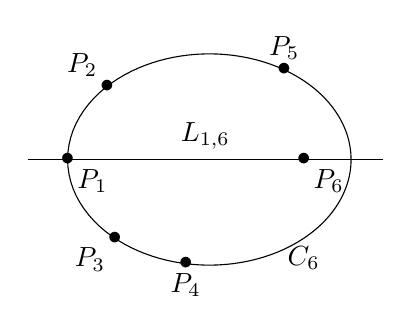
\begin{tikzpicture}[scale=.5]
\coordinate (P_1) at (-6,0);
\coordinate (P_6) at (0,0);

\draw (P_1) node[below right] {$P_1$}
node{$\bullet$} ;
\draw (-5, 1.85) node[above left] {$P_2$} node{$\bullet$};
\draw (-4.8, -2) node[below left] {$P_3$} node{$\bullet$} ;
\draw (-3, -2.64) node[below] {$P_4$} node{$\bullet$};
\draw (-0.5, 2.28) node[above] {$P_5$} node{$\bullet$};
\draw (P_6) node[below right] {$P_6$}
node{$\bullet$} ;

\draw (-7,0) -- (2,0) node[midway,above] {$L_{1,6}$};

\draw [domain= -180 : 180, samples = 200] plot (\x : {3/(1.5 + cos(\x))});
\draw (0,-2.5) node {$C_6$};
\end{tikzpicture}
\]
Now, we consider six points not in generic position. Take four lines $(L_1,\dots,L_4)$ in~$\mathbb{P}_2$ with exactly six intersections $(P_1,\dots,P_6)$, those lines are black in the next figure. Consider the three lines $L_{1,2}, L_{3,4}$ and $L_{5,6}$ with $L_{i,j}$ containing $P_i$ and $P_j$, those lines are blue in the next figure. Up to relabeling we may assume $L_{i,j}\ne L_k$ for all $i,j,k$. Cayley's nodal cubic is obtained by blowing up the six points and then blowing down the strict transforms of the four lines $(L_1,\dots,L_4)$. The four points image of those four lines under the blow-down are exactly the four singular points. See Hunt \cite[Chap.\,4]{Hunt} for more pictures.
\[
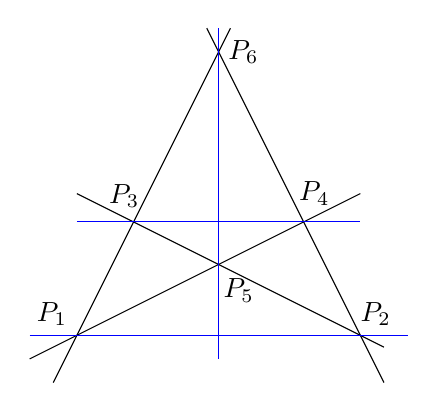
\begin{tikzpicture}[scale=.6]
\draw (-0.5,-1)--(3.25,6.5) ;
\draw (-1,-0.5)--(6,3);
\draw (2.75,6.5)--(6.5,-1);
\draw (0,3)--(6.5,-0.25);

\draw [blue] (-1,0)--(7,0);
\draw [blue] (3,-0.5)--(3,6.5);
\draw [blue] (0,2.4)--(6,2.4);

\draw (0,0) node[above left] {$P_1$};
\draw (1,2.5) node[above] {$P_3$};
\draw (4.5,2.55) node[above right] {$P_4$};
\draw (2.9,1.4) node[below right] {$P_5$};
\draw (3,6) node[right] {$P_6$};
\draw (5.8,0) node[above right] {$P_2$};
\end{tikzpicture}
\]

\begin{proposition}[lines on Cayley's nodal cubic]\label{prop_lines_cayley}
There are $9$ lines on Cayley's nodal cubic.
\begin{itemize}
\item Six of them are the exceptional divisors $E_i$ over $P_i$.
\item Three of them are the strict transforms of $L_{1,2}, L_{3,4}$ and $L_{5,6}$.
\end{itemize}
\end{proposition}
\begin{proposition}
The variety $\mathcal{M}_{\overline{\boldsymbol{\mathcal{C}}}}$ is Cayley's nodal cubic minus the images of $L_{1,2}, L_{3,4}$ and $L_{5,6}$.
\end{proposition}
\begin{proof}
We saw that $\mathcal{M}_{\overline{\boldsymbol{\mathcal{C}}}}$ is Cayley's nodal cubic minus the three lines at infinity $xyz=0$. These three lines do not contain any of the four singularities. Therefore they are not the image of the exceptional divisors. Then they must be the three remaining lines, the blue lines on the picture.
\end{proof}
\begin{theorem}
The character variety $\mathcal{M}_{\boldsymbol{\mathcal{S}}}$ with generic semisimple conjugacy classes at punctures is diffeomorphic to the minimal resolution of singularities of the character variety $\mathcal{M}_{\overline{\boldsymbol{\mathcal{C}}}}$. Both are obtained as the projective plane $\mathbb{P}^2$ blown up in six points $(P_1,\dots,P_6)$ minus three lines $\widetilde{L}_{1,2}, \widetilde{L}_{3,4}, \widetilde{L}_{5,6}$.
\end{theorem}
\begin{proof}
The statement about the minimal resolution of $\mathcal{M}_{\overline{\boldsymbol{\mathcal{C}}}}$ follows from Proposition~\ref{prop_lines_cayley}. The variety $\mathcal{M}_{\boldsymbol{\mathcal{S}}}$ is a smooth projective cubic surface minus three lines forming a triangle. As those three lines intersect each other they cannot be any triple among the $27$ lines over the surface, there are some restrictions:
\begin{itemize}
\item The exceptional divisors $E_i$ do not intersect each other.
\item The strict transforms $\widetilde{C}_j$ do not intersect each other.
\item The strict transforms of two distinct lines containing a same point $P_i$ do not intersect.
\end{itemize}
Therefore the only possible triples of lines forming a triangle on a smooth cubic surface have the following form:
\begin{enumerate}
\item $(\widetilde{L}_{1,2},\widetilde{L}_{3,4}, \widetilde{L}_{5,6})$,
\item $(E_1, \widetilde{L}_{1,6},\widetilde{C}_6) $.
\end{enumerate}
The first case is exactly the expected result. The second case is illustrated by the picture below Proposition \ref{proposition_27}, where the conic $C_6$ and the line $L_{1,6}$ are drawn. To relate the second case to the first, proceed in two steps. First $\mathbb{P}^2$ is blown-up in the three points $P_1, P_2$ and $P_3$. The resulting variety is blown-down along $\widetilde{L}_{1,2},\widetilde{L}_{1,3}$ and $\widetilde{L}_{2,3}$ (three lines with self-intersection $-1$). The variety obtained is again isomorphic to $\mathbb{P}_2$. We consider this copy of the projective plane as the starting point. This plane is blown up in six points $(P_1',\dots,P_6')$ with
\begin{itemize}
\item $P_1'$ the blow-down of $\widetilde{L}_{2,3}$,
\item $P_2'$ the blow-down of $\widetilde{L}_{1,3}$,
\item $P_3'$ the blow-down of $\widetilde{L}_{1,2}$,
\item $P_j'$ the image of $P_j$ for $j=4,5,6$.
\end{itemize}
The construction obtained from the new copy of $\mathbb{P}^2$ and the points $(P_1',\dots,P_6')$ are labeled with a prime. Then the triple $(E_1, \widetilde{L}_{1,6},\widetilde{C}_6) $ becomes $(\widetilde{L}'_{2,3},\widetilde{L}'_{1,6},\widetilde{L}'_{4,5})$. In any case the triangle of lines removed at infinity has the expected form.
\end{proof}
\begin{remark}
There is an action of the Weyl group of $\mathbb{E}_6$ on the configuration of the $27$ lines on a smooth cubic surface. The Dynkin diagram of $\mathbb{E}_6$ is
\[\begin{tikzcd}[scale=.8]
	&& \bullet \\
	\bullet & \bullet & \bullet & \bullet & \bullet
	\arrow[no head, from=2-1, to=2-2, start anchor=center, end anchor = center ]
	\arrow[no head, from=2-3, to=2-4,start anchor=center, end anchor = center ]
	\arrow[no head, from=2-4, to=2-5,start anchor=center, end anchor = center ]
	\arrow[no head, from=1-3, to=2-3,start anchor=center, end anchor = center ]
	\arrow[no head, from=2-2, to=2-3,start anchor=center, end anchor = center ]
\end{tikzcd}
\]
The generator of the upper vertex corresponds to the transformation previously described sending $(E_1, \widetilde{L}_{1,6},\widetilde{C}_6) $ to $(\widetilde{L}'_{2,3},\widetilde{L}'_{1,6},\widetilde{L}'_{4,5})$, see Hartshorne \cite[V, Exer.\,4.11]{Hartshorne}.
\end{remark}

\subsection{Moduli spaces}\label{sect_moduli_spaces}

In general the construction of the diffeomorphism relies on analytical techniques and go through various moduli spaces. Let $\Sigma$ be a compact Riemann surface endowed with a complex structure, then $\Sigma$ is seen as a smooth complex projective curve. Let $D$ be the divisor $D=p_1+\dots +p_k$ for $k$ distinct points $p_1,\dots,p_k$.

\subsubsection{De Rham moduli space}\label{subsect_dR_alg}
Parabolic holomorphic bundles were introduced by Mehta and Seshadri \cite{Mehta_Seshadri}, they generalized Narasimhan--Seshadri \cite{Narasimhan_Seshadri} result to the parabolic case. Parabolic bundles appear in various area of mathematics and physics, for instance Pauly \cite{Pauly} related those parabolic bundles with conformal field theory. In this section some definitions are recalled.

\begin{definition}[Filtered holomorphic bundles]
A filtered holomorphic bundle consists of the data of a holomorphic vector bundle $E$ together with filtrations of $E^j$ the fiber of~$E$ at $p_j$ for $j=1,\dots,k$
\[
\left\lbrace 0\right \rbrace = E^j_0 \subset E^j_1\subset\dots\subset E^j_{m_j} = E^j.
\]
The type $\tau$ of the filtration is defined by
\[
\tau^j_i =\dim E^j_i/E^j_{i-1}
\]
for $j=1,\dots,k$ and $i=1,\dots,m_j$.
\end{definition}
\begin{definition}[parabolic degree]
Let $E$ be a filtered holomorphic bundle of type~$\tau$. Consider a stability parameter $\beta=(\beta^j_i)_{\substack{1\le j \le k \\ 1 \le i \le m_j}}$ with $\beta_i^j\in\mathbb{R}$. The parabolic degree of $E$ is
\[
\pdeg_{\beta} E =\deg E + \sum_{i,j} \beta^j_i \dim(E^j_i/E^j_{i-1}).
\]
\end{definition}

Let $E$ be a holomorphic vector bundle on $\Sigma$. A logarithmic connection on $E$ is a map of sheaves $D: E\to E\otimes \Omega^1_{\Sigma}(\log D)$ satisfying Leibniz rule
\[
D(f s) = df\otimes s + f D(s)
\]
for all holomorphic functions $f$ and for all sections $s$ of $E$.

For a coordinate $z$ vanishing at a point $p_j$, in a trivialization of $E$ in a neighborhood of this point the connection reads
\[
D = d + A(z) \frac{d z}{z}.
\]
The residue of $D$ at $p_j$ is $A(0)$, we denote it by $\Res_{p_j} D$.

Fix some parabolic weights $\beta^j_i\in \left[ 0, 1\right[$ satisfying $\beta^j_i < \beta^j_{i-1}$. For $j=1,\dots, k$ and $i=1,\dots,m_j$, fix $A^j_i \in \C$ to specify a polar part. A logarithmic connection $(E,D)$ is compatible with the parabolic structure if the endomorphism
\[
\Res_{p_j} D : E^j \to E^j
\]
satisfies $\left(\Res_{p_j} D\right) E^j_i \subset E^j_{i}$. A logarithmic connection compatible with the parabolic structure is called a parabolic connection. It is compatible with the specified polar part if in addition the map induced by $\Res_{p_j} D$ on the graded spaces $ E^j_i/E^j_{i-1} $ is $A^j_i \Id$.
A logarithmic connection compatible with the parabolic structure is $\beta$-semistable if and only if, for all subbundles $F\subsetneq E$ preserved by $D$
\[
\frac{\pdeg_{\beta} F}{\rank F} \le \frac{\pdeg_{\beta} E}{\rank E},
\]
it is stable if the inequality is strict unless $F=0$. Two pairs of filtered holomorphic bundles and parabolic connections $(E,D)$ and $(E',D')$ are isomorphic if there is an isomorphism of holomorphic bundle $f:E\to E'$ compatible with the filtrations and such that $\left(f\otimes Id\right)\circ D = D'\circ f$. A connection is flat if its curvature vanishes, this is automatically the case here as we consider logarithmic connections on holomorphic bundles on a Riemann surface.

\begin{notations}[de Rham moduli space]
The de Rham moduli space $\mathcal{M}^{\dR}_{A,\beta}$ classifies isomorphism classes of $\beta$-stable parabolic connections with prescribed polar parts~$A$ and parabolic degree $0$.
\end{notations}

\Subsubsection{Filtered local systems and resolutions of character varieties}\label{subsect_resol_filtered_local}
\begin{definition}[Filtered local system]
A filtered local system is a local system~$\mathcal{L}$ over $\Sigma\setminus\left\lbrace p_1,\dots,p_k\right\rbrace$ together with a filtration of the restrictions $\mathcal{L}_{\left|U_j\right.}$ to some punctured neighborhood $U_j$ of $p_j$. Namely for all $j=1,\dots,k$ there are local systems $\mathcal{L}^j_i$ such that
\[
0 = \mathcal{L}^j_0 \subsetneq \mathcal{L}^j_1 \subsetneq \dots\subsetneq \mathcal{L}^j_{m_j} = \mathcal{L}_{\left|U_j\right.}.
\]
The type $\tau$ of the filtered local system is defined by
\[
\tau^j_i := \rank \mathcal{L}^j_i/ \mathcal{L}^j_{i-1}.
\]
\end{definition}

\begin{definition}[Parabolic degree of a filtered local system]
Let $\gamma =(\gamma^j_i)_{\substack{1\le j \le k \\ 1 \le i \le m_j}}$ be a stability parameter. The parabolic degree of the filtered local system is defined~by
\[
\pdeg_{\gamma} \mathcal{L} = \sum_{i,j} \gamma^j_i \rank \mathcal{L}^j_i / \mathcal{L}^j_{i-1}.
\]
\end{definition}

A filtered local system $\mathcal{L}$ is $\gamma$-semistable if and only if for all sub local systems $ 0 \subsetneq \mathcal{L}' \subsetneq \mathcal{L}$,
\[
\frac{\pdeg_{\gamma} \mathcal{L}'}{\rank \mathcal{L}'} \le \frac{\pdeg_{\gamma} \mathcal{L}}{\rank \mathcal{L}},
\]
it is $\gamma$-stable if the inequality is strict.

Consider a character variety $\mcmus$ with a resolution of singularities $\widetilde{\mathcal{M}}_{\boldsymbol{L},\boldsymbol{P}, \boldsymbol{\sigma}}$. By~the usual equivalence of category between local systems and representations of the fundamental group, the character variety $\mcmus$ is the moduli space of local systems with monodromy around $p_{j}$ in $\overline{\mathcal{C}}_{\underline{\mu}^j,\sigma^j}$. This correspondence extends to the resolution $\mlps$ and the moduli space of filtered local system.
\begin{proposition}\label{proposition_filtered_moduli_resolu}
The resolution $\mlps$ is the moduli space of filtered local systems with filtration around $p_j$ of type ${\underline{\mu}^j}'$ and such that the endomorphism induced by the monodromy on $\mathcal{L}^j_i/\mathcal{L}^j_{i-1}$ is $\sigma^j_i \Id$.
\end{proposition}
\begin{proof}
An element $g_j P^j \in \GL_n /P^j$ is identified with a partial flag of type ${\underline{\mu}^j}'$.
The condition $g_j\inv X_j g_j \in \sigma^j U_{P^j}$
is exactly that the partial flag is preserved by $X_j$
and that the induced endomorphism on the graded spaces are $\sigma_i^j \Id$.
Note that we study only character varieties for generic choices of conjugacy classes at punctures. For such a generic choice, the stability parameter is irrelevant as the local system does not admit any sub local system.
\end{proof}

\subsubsection{Dolbeault moduli space}\label{subsect_dol_alg}
A parabolic Higgs bundle is a pair $(E,\phi)$ with $E$ being a filtered holomorphic vector bundle on $\Sigma$ and a Higgs field $\phi : E \to E\otimes \Omega^1(\log D) $ such that $\Res_{p_j}\phi (E^j_i)\subset E^j_i$. Let $\alpha =(\alpha^j_i)_{\substack{1\le j \le k \\ 1 \le i \le n_j}}$ be a stability parameter. A parabolic Higgs bundle $(E,\phi)$ is $\alpha$-semistable if and only if for all subbundles $0\subsetneq F\subsetneq E$ preserved by $\phi$
\[
\frac{\pdeg_{\alpha} F}{\rank F} \le \frac{\pdeg_{\alpha} E}{\rank E}.
\]
It is $\alpha$-stable if the inequality is strict.
Similarly to the case of parabolic connections, it is interesting to specify the residue of the Higgs field. For all $i,j$, fix a semisimple adjoint orbit $B^j_i$ in $\gl_{\nu^j_i}$. The parabolic Higgs bundle has the prescribed residues if, in~a holomorphic trivialization, the map induced on $E^j_i / E^j_{i-1}$ by the residue lies in the adjoint orbit $B^j_i$. Note that contrarily to the parabolic connections, the prescribed adjoint orbits on the graded spaces are not necessarily central. In fact much more general polar parts are considered by Biquard--Boalch \cite{Biquard_Boalch_2004}, we restrict here to what is necessary for our purpose.

\begin{notations}[Dolbeault moduli space]
The Dolbeault moduli space $\mathcal{M}^{\Dol}_{B,\alpha}$ classifies isomorphism classes of
$\alpha$-stable parabolic Higgs bundles with prescribed residues~$B$ and parabolic degree $0$.
\end{notations}

\subsubsection{Various steps of the diffeomorphism}\label{sect_analytic_moduli}
In the remaining of the section, analytic constructions of the moduli spaces are recalled. These spaces are endowed with a manifold structure. They will be used to obtain a diffeomorphism from a resolution $\widetilde{\mathcal{M}}_{\boldsymbol{L},\boldsymbol{P}, \boldsymbol{\sigma}}$ to a character variety $\mathcal{M}_{\boldsymbol{\mathcal{S}}}$ with semisimple conjugacy classes at punctures. The picture is the following:
\begin{equation}\label{diagram_path_ch4}
\begin{array}{c}
\xymatrix@C=1.5cm{
\widetilde{\mathcal{M}}_{\boldsymbol{L},\boldsymbol{P}, \boldsymbol{\sigma}} \ar[r]^-{\text{R.H}} & \mathcal{M}^{\dR}_{A,\beta} \ar[r]^-{\text{N.A.H}} & \mathcal{M}^{\Dol}_{B,\alpha} \ar[d]^{\alpha\mto \widetilde{\alpha}}\\
\mathcal{M}_{\boldsymbol{\mathcal{S}}} & \ar[l]_-{\text{R.H}} \mathcal{M}^{\dR}_{\widetilde{A},\widetilde{\beta}} &\ar[l]_-{\text{N.A.H}} \mathcal{M}^{\Dol}_{B,\widetilde{\alpha}}.
}
\end{array}
\end{equation}
All the arrows are diffeomorphisms, R.H stands for the Riemann--Hilbert correspondence and N.A.H for non-Abelian Hodge theory. The vertical arrow accounts for a change of stability parameter $\alpha\mto\widetilde{\alpha}$. This is similar to a construction from Biquard, García-Prada and Mundet i Riera \cite[Th.\,7.10]{Biquard_Garcia_Prada_Riera}. It is detailed in the remaining of the section for this particular application.

\subsection{Local model}\label{subsect_local_model}
In this section the local model used by Biquard--Boalch \cite{Biquard_Boalch_2004} to construct moduli spaces is recalled.

\subsubsection{Local model for the Riemann--Hilbert correspondence}\label{subsub_local_RH}
Before constructing the moduli spaces, let us present what happens locally, near a puncture, and how the parameters of the moduli spaces are related. Consider a rank $n$ filtered local system~$\mathcal{L}$ on a punctured disk $\mathbb{D}^0=\lbrace z\in \mathbb{C} \mid 0 < |z|< 1\rbrace$. We assume that the monodromy induces a central endomorphism on the successive quotients of the filtration. The monodromy $X$ has eigenvalues $\sigma_i$ with multiplicity $\nu_i$ for $1\le i \le l$. We assume the filtration of the local system is finer than a filtration spanned by generalized eigenspaces of $M$. Then in a trivialization $(l_j)_{1\le j \le n}$ compatible with the filtration, the monodromy reads
\[\arraycolsep2.5pt
X =
\begin{pmatrix}
X_{\sigma_1} & *& \\
0 & X_{\sigma_2} & *\\
\vdots & 0 & \ddots
\end{pmatrix}
\]
with $X_{\sigma_i}$ being a block of size $\nu_i$ with further decomposition
\[\arraycolsep2.5pt
X_{\sigma_i} =
\begin{pmatrix}
\sigma_i \Id_{{\mu^i_1}'} & *& \\
0 & \sigma_i \Id_{{\mu^i_2}'} & *\\
\vdots & 0 & \ddots
\end{pmatrix}.
\]
The type of the filtration is $\underline{\mu}'=({\mu^1_1}',{\mu^1_2}',\dots,{\mu^2_1}',{\mu^2_2}',\dots)$. Let $A_i \in \C$ be such that
\[
\exp(- 2 i \pi A_i)=\sigma_i
\]
and $0 \le \Ree A_i<1$. Then $A$ is the diagonal matrix with diagonal entries
\[
\bigl(\underbrace{A_1,\dots,A_1}_{\nu_1},\dots,\underbrace{A_l,\dots,A_l}_{\nu_l}\bigr).
\]
Let $a$ be a block strictly upper triangular matrix such that $\exp\left(-2i\pi (A+a)\right)=X$. Define $E$ a rank $n$ holomorphic bundle on the disk $\mathbb{D}=\lbrace z\in\mathbb{C} \mid |z|<1\rbrace$ spanned by $\tau_j=e^{(A+a) \log z} l_j$ for $1\le j\le n$. Let $D$ be the parabolic connection on $E$ defined in the holomorphic trivialization $(\tau_j)_{1\le j\le n}$ by
\[
D = d + \frac{A+a}{z}\, dz = D_0 + \frac{a}{z}\, dz.
\]
Then the filtered local system $\mathcal{L}$ is nothing but the local system of flat sections of the parabolic connection $(E,D)$. This describes locally the Riemann--Hilbert correspondence between a resolution of a character variety and a de Rham moduli space.

\subsubsection{Metric and parabolic structure}
The connection $D_0$ will be the local model for parabolic connections
\[
D_0 = d + \frac{A}{z}\, dz,
\]
with $A$ diagonal. In order to continue the path presented in Diagram \eqref{diagram_path_ch4}, we need to introduce a Hermitian metric. It will be related to a choice of stability parameters. Chose some stability parameters $\beta_{r,s}\in [0,1[$ for each graded space of the filtration of type $\underline{\mu}$. We introduce a diagonal matrix $\beta$ with diagonal coefficients
\[
(\beta_1,\beta_2,\dots,\beta_n := \Bigl(\overbrace{\underbrace{\beta_{1,1},\dots,\beta_{1,1}}_{{\mu^1_1}'},\underbrace{\beta_{1,2},\dots,\beta_{1,2}}_{{\mu^1_2}'},\dots}^{\nu_1},\dots,\overbrace{\underbrace{\beta_{l,1},\dots,\beta_{l,1}}_{{\mu^l_1}'},\dots }^{\nu_l} \Bigr)
\]
so that the $\beta_i$ are the $\beta_{r,s}$ repeated according to the multiplicities ${\mu^r_s}'$. Moreover, assume that $\beta_i \ge \beta_{i+1}$ and $\beta_{r,s}\ne \beta_{u,v}$ if $(r,s)\ne(u,v)$.
\begin{remark}\label{remark_various_beta}
In this local model there is just one puncture $p_1$, therefore the stability parameters introduced in \ref{subsect_dR_alg} are $(\beta^1_i)_{1\le i \le m_1}$. They are related to the stability parameters introduced in this section by
\[
(\beta^1_1,\beta^1_2,\dots,\beta^1_{m_1})=(\beta_{1,1},\beta_{1,2},\dots,\beta_{2,1},\beta_{2,2},\dots).
\]
We apologize for the multiplication of similar notations. The parameters $(\beta^1_i)_{1\le i \le m_1}$ are adapted to the algebraic definition of stability whereas $(\beta_{r,s})_{\substack{1\le r \le l \\ 1 \le s \le \mu^r_1 }}$ are adapted to the description of the connections and $(\beta_1,\beta_2,\dots,\beta_n)$ is adapted to explicit constructions of trivializations.
\end{remark}
Define a Hermitian metric $h$ on $E$ such that $|\tau_j| = |z|^{\beta_j}$. This metric determines the filtration of $E$:
\[
E_i = \bigl\lbrace s\in E \mid | s(z) |_h = \mathcal{O}\bigl(| z|^{\beta^1_i}\bigr)\bigr\rbrace.
\]
with $|\csbullet|_h$ being the norm with respect to the metric $h$. We obtain a Hermitian vector bundle $\mathbb{E}$ on the disk $\mathbb{D}$ with an orthonormal trivialization $(\sfrac{\tau_j}{|z|^{\beta_j}})_{1\le j \le n}$.
\begin{notations}
The symbol $\mathbb{E}$ represents a vector bundle in the sense of differential geometry, with smooth transition functions; whereas the symbol $E$ represents a holomorphic bundle.
\end{notations}
The parabolic connection $D_0$ on the holomorphic bundle $E$ induces a connection on $\mathbb{E}$, in the orthonormal trivialization $(\sfrac{\tau_j}{|z|^{\beta_j}})_{1\le j \le n}$ it reads
\[
D_0 = d + \Bigl(A -\frac{\beta}{2}\Bigr) \frac{d z}{z} -\frac{\beta}{2} \frac{d \overline{z}}{\overline{z}}.
\]

\subsubsection{Local behaviour for non-Abelian Hodge theory}\label{subsection_local_naht}
The connection $D_0$ decomposes as a unitary connection plus a self-adjoint term
\[
D_0= D_0^h + \Phi_0.
\]
In the orthonormal trivialization $(\sfrac{\tau_j}{|z|^{\beta_j }})_{1\le j \le n}$,
\[
D_0^h = d + \frac{A}{2} \frac{d z}{z} - \frac{A^{\dagger}}{2} \frac{d\overline{z}}{\overline{z}}
\]
and
\[
\Phi_0 = \frac{1}{2} \Bigl(A\frac{d z}{z} + A^{\dagger}\frac{d\overline{z}}{\overline{z}} - \beta \frac{d z}{z} - \beta \frac{d \overline{z}}{\overline{z}}\Bigr).
\]
Consider the basis $(e_j)_{1\le j \le n} $ defined by
\[
e_j := \frac{\tau_j}{\left|z\right|^{\beta_j- i \Imm A_j}},
\]
with $\Imm A_j$ being the imaginary part of the $j$-th diagonal term of the matrix $A$.
\begin{notations}[Canonical form]\label{notations_canonical_form}
The expression of $D_0$ in the orthonormal trivialization $(e_j)_{1\le j\le n}$ is
\begin{align*}
D_0 &= D_0^h + \Phi_0,\\
D_0^h &= d +\frac{1}{2} \Ree (A) \Bigl(\frac{d z}{z}- \frac{d\overline{z}}{\overline{z}}\Bigr),\\
\Phi_0 &= \frac{1}{2} \Bigl(A\frac{d z}{z} + A^{\dagger}\frac{d\overline{z}}{\overline{z}} - \beta \frac{d z}{z} - \beta \frac{d \overline{z}}{\overline{z}}\Bigr).
\end{align*}
Such expressions will be referred to as canonical forms.
\end{notations}
Let $\overline{\partial}^F$ be the $(0,1)$-part of $D_0^h$ and let $\theta_0$ be the $(1,0)$-part of $\Phi_0$. In the basis $(e_j)_{1\le j \le n} $ one has
\[
\overline{\partial}^F = \drond - \frac{1}{2} \Ree (A) \frac{d\overline{z}}{\overline{z}}.
\]
This operator defines a holomorphic bundle over the punctured disk with holomorphic sections killed by $\drond^F$. This holomorphic bundle can be extended over the puncture to a holomorphic bundle $F$, by taking as a basis of holomorphic sections $(f_j)_{1\le j \le n}$ defined by
\[
f_j = |z|^{\alpha_j} e_j,
\]
where $\alpha_j$ is the real part of the $j$-th diagonal term of the matrix $A$. Then
\[
|f_j|_h = \left|z\right|^{\alpha_j}.
\]
As in Remark \ref{remark_various_beta}, we associate a stability parameter $(\alpha^1_i)_{1\le i \le n_1}$ to $(\alpha_1,\dots,\alpha_n)$.
This stability parameter provides a parabolic structure
\[
F_i =\lbrace s\in F\mid |s|_h=\mathcal{O}(|s(z)|^{\alpha_i^1})\rbrace.
\]
Note that the holomorphic bundle $F$ is different from the holomorphic bundle $E$. Even the types of the parabolic structures differ, $E$ is of type $\underline{\mu}'$ whereas $F$ is of type~$\nu$.

Note that $\theta_0$, the $(1,0)$ part of $\Phi_0$, provides a Higgs field
\[
\theta_0 = \frac{1}{2} \left(A - \beta\right)\frac{d z}{z}.
\]
This is the local behaviour of the non-Abelian Hodge theory for the model connection.
To summarize, starting from a flat parabolic connection $D_0$ with polar part $A$, a~metric~$h$ and a parabolic structure $\beta$ we obtain a parabolic Higgs bundle with residue of the Higgs field $B$ and parabolic structure $\alpha$. The relations between those parameters are as described by Simpson \cite{Simpson}
\begin{equation}\label{eq_nah_parameters}
\begin{split}
B &= \frac{1}{2}(A - \beta),\\
\alpha &= \Ree A.
\end{split}
\end{equation}

\Subsubsection{Local description of weighted Sobolev spaces}\label{subsect_local_weighted}
\begin{definition}[Weighted $L^2$ spaces]
The radial coordinate on the disk is $r=|z|$. For $\delta$ real, let $L^2_{\delta}$ be the space of functions $f$ on the disk such that $\sfrac{f}{r^{\delta+1}}$ is $L^2$.
\end{definition}
The Hermitian metric $h$ on the vector bundle $\mathbb{E}$ induces a metric on $\End (\mathbb E)$ and $\End (\mathbb E)\otimes \Omega^1$. The definition of the spaces $L^2_{\delta}$ extends to sections of such bundles using the induced metric. There is an orthogonal decomposition
\begin{equation}\label{eq_end_E}
\End(\mathbb{E}) = \End(\mathbb{E})_0 \oplus \End(\mathbb{E})_1,
\end{equation}
with $\End(\mathbb{E})_0$ being the space of endomorphism commuting with $A$. It induces an orthogonal decomposition
\[
\Omega^1 \otimes \End(\mathbb{E}) =(\Omega^1 \otimes \End (\mathbb{E})_0) \oplus(\Omega^1 \otimes \End (\mathbb{E})_1).
\]
For $f\in \Omega^1\otimes \End(\mathbb{E}) $ this orthogonal decomposition reads
\[
f=f_0 +f_1.
\]

\begin{definition}[Sobolev spaces $L^{k,2}_{\delta}$]
The weighted Sobolev space is defined by
\[
L^{k,2}_{\delta}(\Omega^1\otimes\End (\mathbb{E})) :=\bigl\lbrace f \in L^2_{\delta} \mid \nabla^j f_0, \; \sfrac{\nabla^j f_1}{r^{k-j}} \in L^{2}_{\delta} \; \text{ for }0\le j \le k\bigr\rbrace,
\]
with $\nabla$ being the covariant derivative with respect to the unitary connection $D_0^h$.
\end{definition}

\begin{definition}[Space of admissible connections]\label{def_admissible_connections_loc}
The space of admissible connections is
\[
\mathcal{A} =\lbrace D_0+a \mid a \in L^{1,2}_{-2+\delta}(\Omega^1\otimes \End (\mathbb{E}))\rbrace.
\]
\end{definition}
\begin{remark}
Note that the space of admissible connections is chosen so that the connection $D=D_0+a$ introduced at the beginning of this section is admissible. Indeed, in the orthonormal trivialization $\left(e_j\right)_{1\le j \le n}$, the matrix $a$ is strictly block upper triangular. The non zero coefficients strictly above the diagonal have the following form
\[
|z|^{\beta_i-\beta_j} \frac{a_{i,j}}{z},
\]
with $\beta_i > \beta_j$ and $a_{i,j}$ constant. Thus $a\in L^{1,2}_{-2+\delta}$ for a small enough parameter:
\[
0<\delta < \beta_i-\beta_j.
\]
\end{remark}

\subsubsection{Variation of the stability parameter and the metric}\label{subsect_local_variation_metric}
In order to pursue the path announced in Diagram \eqref{diagram_path_ch4}, we slightly modify the stability parameter $\alpha$ to a parameter $\widetilde{\alpha}$, it is identified with a diagonal matrix with coefficients
\[
(\widetilde{\alpha}_1,\widetilde{\alpha}_2,\dots)=\bigl(\underbrace{\widetilde{\alpha}_{1,1},\dots, \widetilde{\alpha}_{1,1}}_{{\mu^1_1}' }, \underbrace{\widetilde{\alpha}_{1,2},\dots, \widetilde{\alpha}_{1,2}}_{ {\mu^1_2}'}, \dots \bigr).
\]
The associated metric $\widetilde{h}$ is defined such that the holomorphic trivialization $(f_j)_{1\le j\le n}$ of the holomorphic bundle $F$ is orthogonal and
\[
|f_j|_{\widetilde{h}} =|z|^{\widetilde{\alpha}_j}.
\]
This provides a Hermitian bundle with orthonormal trivialization $(\widetilde{e}_j)_{1\le j\le n}$ defined~by
\[
\widetilde{e}_j = \frac{f_j}{|z|^{\widetilde{\alpha}_j}}.
\]
We follow the same process as before in the opposite direction. The connection $D_0^{\widetilde{h}}$ is the $\widetilde{h}$-unitary connection with $(0,1)$-part $\overline{\partial}^F$, and
\[
\widetilde{\Phi}_0 := \theta_0 + \theta_0^{\widetilde{\dagger}},
\]
where the adjoint is taken with respect to the metric $\widetilde{h}$. Then
\[
\widetilde{D}_0 := D_0^{\widetilde{h}} + \widetilde{\Phi}_0.
\]
In the trivialization $(\widetilde{e}_j)_{1\le j\le n}$ it reads
\begin{align*}
\widetilde{\Phi}_0 &= \frac{1}{2}\left(A-\beta\right)\frac{d z}{z} + \frac{1}{2}(A^{\widetilde{\dagger}}-\beta)\,\frac{d \overline{z}}{\overline{z}}, \\
D_0^{\widetilde{h}} &= d + \frac{1}{2}\widetilde{\alpha} \Bigl(\frac{d z}{z}-\frac{d\overline{z}}{\overline{z}}\Bigr).
\end{align*}
Setting $\widetilde{A}= \widetilde{\alpha}+i \Imm A$ and $\widetilde{\beta}= \beta + \widetilde{\alpha} - \alpha$ we obtain a canonical form as in Notations~\ref{notations_canonical_form}
\begin{align*}
D_0^{\widetilde{h}}= d + \frac{1}{2}\Ree(\widetilde{A})\Bigl(\frac{d z}{z}-\frac{d \overline{z}}{\overline{z}}\Bigr), \\
\widetilde{\Phi}_0 = \frac{1}{2}\Bigl(\widetilde{A}\frac{d z}{z} + \widetilde{A}^{\widetilde{\dagger}}\frac{d\overline{z}}{\overline{z}} - \widetilde{\beta} \frac{d z}{z} - \widetilde{\beta} \frac{d \overline{z}}{\overline{z}}\Bigr).
\end{align*}
Continuing in the opposite direction, the $(0,1)$-part of $\widetilde{D}_0$ defines a holomorphic bundle $\widetilde{E}$ with holomorphic trivialization $(\widetilde{\tau}_j)_{1\le j\le n}$ such that
\[
\widetilde{\tau}_j:=|z|^{\widetilde{\beta}_j- i \Imm \widetilde{A}_j} \widetilde{e}_j.
\]
The operator $\widetilde{D}_0$ defines a logarithmic connection on $\widetilde{E}$, in the trivialization $(\widetilde{\tau}_j)_{1\le j\le n}$ it reads
\[
\widetilde{D}_0 = d + \widetilde{A}\,\frac{d z}{z}
\]
and $\widetilde{A}$ has distinct eigenvalues on each graded of the filtration of type $\nu$ and so does the monodromy of the local system of flat sections.

Let us summarize the local behaviour for Diagram \eqref{diagram_path_ch4} in terms of residue. We~look at a particular block of size $\nu_j$. The stability parameter associated to the graded of the filtration is specified with over-brace. N.A.H stands for non-Abelian Hodge theory.
\[
\xymatrix@C=1.5cm{
\hbox{$\begin{pmatrix}
\overbrace{A_j \Id_{ {\mu^j_{1}}' }}^{\beta_{j,1}} & *& \\
0 & \overbrace{A_j \Id_{ {\mu^j_{2}}' }}^{\beta_{j,2}} & *\\
\vdots & 0 & \ddots
\end{pmatrix}$} \ar[r]^-{\text{N.A.H}} &
\dfrac{1}{2}\left(
\overbrace{
\begin{array}{ccccc}
(A_j-\beta_{j,1}) \Id_{ {\mu^j_{1}}' } & * & \\
0 & (A_j-\beta_{j,2}) \Id_{ {\mu^j_{2}}' } & * \\
\vdots & 0 & \ddots
\end{array}
}^{\alpha^1_j }
\right) \ar[d]^{\alpha \mto \widetilde{\alpha}} \\
\hbox{$\begin{pmatrix}
\overbrace{\widetilde{A}_{j,1} \Id_{ {\mu^j_{1}}' }}^{\widetilde{\beta}_{j,1}} & *& \\
0 & \overbrace{\widetilde{A}_{j,2} \Id_{ {\mu^j_{2}}' }}^{\widetilde{\beta}_{j,2}} & *\\
\vdots & 0 & \ddots
\end{pmatrix}$} & \ar[l]_-{\text{N.A.H}}
\dfrac{1}{2}\hbox{$\begin{pmatrix}
\overbrace{\left(A_j-\beta_{j,1}\right) \Id_{ {\mu^j_{1}}' }}^{\widetilde{\alpha}_{j,1}} & *& \\
0 & \overbrace{\left(A_j-\beta_{j,2}\right) \Id_{{\mu^j_{2}}' }}^{\widetilde{\alpha}_{j,2}} & *\\
\vdots & 0 & \ddots
\end{pmatrix}$}
}
\]

With $\widetilde{A}_{j,i}= \widetilde{\alpha}_{j,i}+ i \Imm A_j$ and $\widetilde{\beta}_{j,i}=\beta_{j,i}+\widetilde{\alpha}_{j,i}-\alpha^1_j$.

\Subsection{Diffeomorphism between moduli spaces}\label{sect_diffeo_ms}
\subsubsection{Analytic construction of the moduli spaces}\label{sect_global_moduli}
The local study on the disk actually extends to global moduli spaces for objects defined over punctured Riemann surfaces. The analytic construction of moduli spaces relies on methods from Kuranishi \cite{Kuranishi}, Atiyah--Hitchin--Singer \cite{Atiyah_Hitchin_Singer} and Atiyah--Bott \cite{Atiyah_Bott}. In this section we recall the analytic construction of the moduli spaces involved in the parabolic version of non-Abelian Hodge theory. Some particular cases of those moduli spaces were constructed by Konno \cite{Konno} and Nakajima \cite{Nakajima_1996}. However we need a more general construction in order to allow not necessarily central action of the residues of the Higgs fields on the graded of the filtration. The construction we follow is the one from Biquard--Boalch \cite{Biquard_Boalch_2004}. Note that a larger family of groups was considered by Biquard, García-Prada and Mundet i Riera \cite{Biquard_Garcia_Prada_Riera}.

The local canonical model introduced in \ref{notations_canonical_form} is used to represent behaviour of connections near the punctures $p_j$. Let $\mathbb{E}$ be a vector bundle on $\Sigma$ endowed with a Hermitian metric $h$. The notation $\mathbb{E}$ refers to a vector bundle from the differential geometry point of view whereas $E$ refers to a holomorphic bundle. Let $D_0$ be a model connection such that on the neighborhood of the punctures it coincides with the local model connection of the previous subsection. The connection decomposes as
\[
D_0 = D_0^h + \Phi,
\]
with $D_0^h$ unitary and $\Phi$ self-adjoint with respect to the metric $h$. We assume for this model connection that in an orthonormal trivialization $(e_i)_{1\le i \le n}$ of $\mathbb{E}$ near the puncture $p_j$,
\[
D^h_0 = d + \frac{1}{2} \Ree(A^j) \Bigl(\frac{d z}{z} - \frac{d \zbar}{\zbar}\Bigr)
\]
and
\[
\Phi = \frac{1}{2} \Bigl(A^j\frac{d z}{z} + (A^j)^{\dagger}\frac{d\overline{z}}{\overline{z}} - \beta^j \frac{d z}{z} - \beta^j \frac{d \overline{z}}{\overline{z}}\Bigr),
\]
where $A^j$ and $\beta^j$ are the residue and the stability parameter for the de Rham moduli space at the puncture $p_j$. They correspond to the local parameter $A$ and $\beta$ from Section~\ref{subsect_local_model}, they are constant diagonal matrices. The parameter of the de Rham moduli space is chosen so that it corresponds under the Riemann--Hilbert correspondence to a resolution of a character variety with generic monodromies $\mlps$. Therefore connections with such polar parts are necessarily irreducible.

Take $r$ a function strictly positive on the punctured Riemann surface $\Sigma^0$ such that it coincides with the radial coordinate near each punctures. The global weighted Sobolev space is defined as the local one from \ref{subsect_local_weighted} with this positive function $r$. It~is still denoted by $L^{k,2}_{\delta}(\Omega^1\otimes \End{(\mathbb{E})})$. The space of admissible connections is
\[
\mathcal{A} =\lbrace D_0 + a \mid a \in L^{1,2}_{-2+\delta}(\Omega^1\otimes \End(\mathbb{E}))\rbrace.
\]
This affine space is actually endowed with various complex structures. Decomposing according to $(1,0)$-part and $(0,1)$-part, $a=a^{1,0}+a^{0,1}$. The complex structure $I$ is defined by
\[
I\cdot a = i a
\]
and the complex structure $J$ is defined by
\[
J\cdot a = i(a^{0,1})^{\dagger}-i(a^{1,0})^{\dagger}.
\]
The curvature of an admissible connection $D=D_0 + a$ is denoted by $F_D$. Consider the complex gauge group
\[
\mathcal{G}^I=\lbrace g\in\Aut(\mathbb{E}) \mid (D_0^h g) g\inv, \; g \Phi_0 g\inv \in L^{1,2}_{-2+\delta}\rbrace,
\]
it acts on $ \mathcal{A}$ by
\[
g\cdot D := g D g\inv = D -(D g)g\inv.
\]
The next theorem gives an analytic construction of the set of isomorphism classes of parabolic flat connections with prescribed polar parts. Later on, this set will be endowed with a manifold structure.

\begin{theorem}[Biquard--Boalch {\cite[\S8]{Biquard_Boalch_2004}}]
The de Rham moduli space of stable flat connections with prescribed polar parts on the graded part of the filtration introduced in \ref{subsect_dR_alg} is the following set
\[
\mathcal{M}^{\dR}_{A, \beta} =\lbrace D_0 + a \in \mathcal{A} \mid F_D =0\rbrace/ \mathcal{G}^{I},
\]
where $F_D$ is the curvature of $D=D_0+a$. The stability condition does not appear as it is imposed by the generic choice of eigenvalues of the residue of $D_0$.
\end{theorem}

Now, starting from $ D=D_0 +a \in \mathcal{A}$ there is a natural candidate to produce a parabolic Higgs bundle, like in the local model. First decompose $D$ in a unitary part and a self-adjoint part
\[
D =D^h + \Phi= D_0^h +\frac{a-a^{\dagger}}{2} + \Phi_0 + \frac{ a + a^{\dagger}}{2}.
\]
The natural candidate for the underlying holomorphic structure of the parabolic Higgs bundle is, in the orthonormal trivialization $(e_j)_{1\le j \le k}$,
\[
\overline{\partial}^E = \overline{\partial} - \frac{1}{2} \Ree(A) \frac{d\overline{z}}{\overline{z}} + \frac{a^{0,1}-(a^{1,0})^{\dagger}}{2}.
\]
And the Higgs field is
\[
\theta = \theta_0 + \frac{a^{1,0} + (a^{0,1})^{\dagger}}{2}.
\]
These data provide a Higgs bundle if $\overline{\partial}^E \theta =0$, equivalently if the pseudo curvature~$G_D$ vanishes. Note that the complex structure $J$ is compatible with the Higgs bundles point of view. Indeed, if $\theta$ is the Higgs field associated to $D$ then $i \theta$ is the Higgs field associated to $J\cdot D$. The complex gauge group acts on the Higgs bundles structures~by
\[
g\cdot(\overline{\partial}^E,\theta) :=(g \overline{\partial}^E g\inv,g \theta g\inv).
\]

The next theorem gives an analytic construction of the set of isomorphism classes of parabolic Higgs bundles with prescribed residues.
Later on, this set will be endowed with a manifold structure.
\begin{theorem}[Biquard--Boalch {\cite[\S7]{Biquard_Boalch_2004}}]
The Dolbeault moduli space of stable parabolic Higgs bundles with prescribed polar parts on the graded parts of the filtration introduced in \ref{subsect_dol_alg} is the following set
\[
\mathcal{M}^{\Dol}_{B, \alpha} =\lbrace D_0 + a \in \mathcal{A} \mid \overline{\partial}^E \theta =0\rbrace/ \mathcal{G}^{J}.
\]
The stability condition does not appear as it is imposed by the generic choice of eigenvalues of the residue. As a group, $\mathcal{G}^J$ is just $\mathcal{G}^I$, we change the upper index to precise which action is considered, the $I$-linear action or the $J$-linear action.
\end{theorem}

The non-Abelian Hodge theory gives a correspondence between the Dolbeault moduli space and the de Rham moduli space. The parameters are intertwined as in the local model. A nice way to state this correspondence is with hyperkähler geometry. We introduce the unitary gauge group
\[
\mathcal{G}=\lbrace g\in U(\mathbb{E}) \mid(D_0 g) g\inv \in L^{1,2}_{-2+\delta}\rbrace.
\]
Consider the moduli space
\[
\mathcal{M}=\lbrace D\in\mathcal{A} \mid \overline{\partial}^E \theta=0, \; F_D=0\rbrace/\mathcal{G}.
\]
The equations defining $\mathcal{M}$ can be interpreted as the vanishing of a hyperkähler moment map. Then the moduli space $\mathcal{M}$ is an hyperkähler reduction as in \cite{Hitchin_Karlhede_Lindstrom_Rocek}.
\begin{theorem}[Biquard--Boalch \cite{Biquard_Boalch_2004} Theorem 5.4]
The moduli space $\mathcal{M}$ carries a hyperkähler manifold structure.
\end{theorem}
\begin{proof}
The deformation theory for the moduli space $\mathcal{M}$ at a point $[D]$ is encoded in the following complex
\[
L^{2,2}_{-2+\delta}(\mathfrak{u}(\mathbb{E})) \To{D} L^{1,2}_{-2+\delta}(\Omega^1\otimes\End \mathbb{E}) \To{D+D^*} L^{2}_{-2 +\delta} \bigl((\Omega^2\otimes \End \mathbb{E})\oplus i\mathfrak{u}(\mathbb{E})\bigr).
\]
The operator $D^*$ is the formal adjoint of $D$ with respect to the $L^2$ inner product and the metric $h$. The analytic study of this complex is detailed in \cite{Biquard_Boalch_2004}. Its first cohomology group is represented by the harmonic space $\boldsymbol{H}^1 \subset L^{1,2}_{-2+\delta} \left(\Omega^1\otimes\End \mathbb{E}\right) $. The Kuranishi slice at $[D]$ is defined by
\begin{equation}\label{eq_kuranishi_slice}
\mathcal{S}_D :=\lbrace D+a \mid \Imm(D^* a)= 0, \; G_{D+a}=0, \; F_{D+a}=0\rbrace.
\end{equation}
Taking a small enough neighborhood of $D$ in the Kuranishi slice, one obtains a finite dimensional manifold transverse to the $\mathcal{G}$-orbits. The Kuranishi map provides an isomorphism between a neighborhood of $0$ in $\boldsymbol{H}^1$ and a neighborhood of $D$ in the Kuranishi slice, see Konno \cite[Lem.\,3.8, Th.\,3.9]{Konno}. This provides a hyperkähler manifold structure on the moduli space.
\end{proof}

Now, the non-Abelian Hodge theory can be described the following way.
\begin{theorem}[Biquard--Boalch \cite{Biquard_Boalch_2004} Theorem 6.1]
The manifold $\mathcal{M}$ endowed with the complex structure $I$ is the moduli space $\mathcal{M}^{\dR}_{A,\beta}$. The manifold $\mathcal{M}$ endowed with the complex structure $J$ is the moduli space $\mathcal{M}^{\Dol}_{B,\alpha}$.
\end{theorem}

\Subsubsection{Construction of the diffeomorphisms}
\begin{theorem}[The Riemann--Hilbert correspondence]
The moduli space $\mathcal{M}^{\dR}_{A,\beta}$ is complex analytically isomorphic to a resolution of character varieties $\mlps$.
\end{theorem}
\begin{proof}
As explained in \ref{proposition_filtered_moduli_resolu}, the variety $\mlps$ is nothing but the moduli space of filtered local systems with prescribed graded parts of the monodromies around the punctures. A filtered version of the Riemann--Hilbert correspondence is established as an equivalence of category by Simpson \cite{Simpson}. Yamakawa \cite{Yamakawa} proved that it is a diffeomorphism using a particular construction of the de Rham moduli space from Inaba \cite{Inaba13}. The same argument holds with the de Rham moduli space endowed with the manifold structure from $\mathcal{M}$. Starting from a flat connection, the associated local system is obtained by taking flat sections, \ie by solving a differential equation. When the parameters of the equation vary complex analytically, so does the solution.
\end{proof}

The moduli spaces $\mathcal{M}^{dR}_{A,\beta}$ and $\mathcal{M}^{\Dol}_{B,\alpha}$ are diffeomorphic as both are $\mathcal{M}$ with a particular complex structure. The first line in the path announced in Diagram \ref{diagram_path_ch4} is now constructed. The second line is obtained exactly like the first, but in the other direction. It remains to describe the vertical arrow between two Dolbeault moduli spaces $\mathcal{M}^{\Dol}_{B,\alpha}$ and $\mathcal{M}^{\Dol}_{B,\widetilde{\alpha}}$. This is given by Biquard, García-Prada and Mundet i Riera \cite[Th.\,7.10]{Biquard_Garcia_Prada_Riera}. The construction of the diffeomorphism is detailed in the remaining of the section.

Because of genericity of the eigenvalues of the residue, the stability parameter~$\alpha$ is irrelevant. The parameter $\alpha$ can be changed to a stability parameter $\widetilde{\alpha}$ with different values for each graded of the filtration. Namely one can chose $\widetilde{\alpha}$ such that the associated matrix satisfies $Z_{\GL_n}(\widetilde{\alpha}^{i})=Z_{\GL_n}(B^i)$ and such that the parabolic degree remains $0$. The local behaviour near each puncture is described by the right hand side of the diagram at the end of Section~\ref{subsect_local_variation_metric}.

We introduce the following notation
\[
\epsilon_i := \widetilde{\alpha}_i-\alpha_i.
\]
For the construction of the diffeomorphism in Theorem \ref{th_diffeo_var_alpha}, it will be convenient to assume
\[
\max_{i,j}|\epsilon_i-\epsilon_j| < \delta,
\]
with $\delta$ being the parameter appearing in the weighted Sobolev space $L^{1,2}_{-2+\delta}$.
\begin{proposition}\label{prop_bijection_dol}
For such a choice of parameters there is a natural bijection between $\mathcal{M}^{\Dol}_{B,\alpha}$ and $\mathcal{M}^{\Dol}_{B,\widetilde{\alpha}}$.
\end{proposition}
\begin{proof}
The moduli space $\mathcal{M}^{\Dol}_{B,\alpha}$ classifies isomorphism classes of parabolic Higgs bundles with parabolic structure at $p_j$
\[
0= F^j_0 \subsetneq F^j_1 \subsetneq \dots \subsetneq F^j_{n_j}=F^j,
\]
and with the residue of the Higgs fields preserving this filtration and acting as a semisimple endomorphism $B^j_i$ on the graded spaces
\[
F^j_i / F^j_{i-1}.
\]
Such spaces decompose as direct sum of eigenspaces for $B^j_i$. After ordering the eigenvalues, we obtain a uniquely determined refinement of the initial parabolic structure
\[
0 = \widetilde{F}^j_0 \subsetneq \widetilde{F}^j_1 \subsetneq \dots \subsetneq \widetilde{F}^j_{m_j} = F^j.
\]
Then the residue of the Higgs field acts as a central endomorphism on the graded $\widetilde{F}^j_i / \widetilde{F}^j_{i-1}$.
This gives a map $f:\mathcal{M}^{\Dol}_{B,\alpha}\to \mathcal{M}^{\Dol}_{B,\widetilde{\alpha}}$. Stability is not an issue as the polar part of the residue is generic. The map forgetting part of the filtration is an inverse so that there is a natural bijection between both moduli spaces.
\end{proof}

Before proving that this bijection is a diffeomorphism, we detail the manifold structure on $\mathcal{M}_{B,\widetilde{\alpha}}^{\Dol}$. It is constructed just like $\mathcal{M}^{\Dol}_{B,\alpha}$ but with different parameters.

We construct a moduli space $\mathcal{M}_{\widetilde{h}}$ similar to $\mathcal{M}$. Instead of the initial metric $h$, we~use a metric $\widetilde{h}$, similar to the local model from \ref{subsect_local_variation_metric}. Namely, we chose it so that near each puncture it admits as an orthonormal trivialization $(\widetilde{e}_i)_{1\le i \le n}$ with
\[
\widetilde{e}_i = r^{\epsilon_i} e_i,
\]
where $(e_i)_{1\le i \le n}$ is the orthonormal trivialization with respect to $h$ near the puncture and $\epsilon_i=\widetilde{\alpha}_i-\alpha_i$.

First we construct $\widetilde{D}_0$, a starting point to construct an affine space of admissible connections. Recall that
\[
D_0 = D_0^h +\Phi_0,
\]
where $D_0^h$ is a $h$-unitary connection and $\Phi_0$ is self-adjoint with respect to $h$. Take ${D^h_0}{}''$ the $(0,1)$-part of $D_0^h$ and $\Phi_0^{1,0}$ the $(1,0)$-part of $\Phi_0$. There exists a unique ${D^{\widetilde{h}}_0}{}'$ such that ${D^{\widetilde{h}}_0}{}'+{D^h_0}{}''$ is $\widetilde{h}$-unitary. Let ${\Phi_0^{1,0}}^{\widetilde{\dagger}}$ be the adjoint of $\Phi_0^{1,0}$ with respect to the metric $\widetilde{h}$. Then $\widetilde{D}_0$ is defined by
\[
\widetilde{D}_0 := {D^{\widetilde{h}}_0}{}'+{D^h_0}{}''+ \Phi_0^{1,0} + {\Phi_0^{1,0}}^{\widetilde{\dagger}}.
\]
Near the puncture, in the trivialization $(\widetilde{e}_i)_{1\le i \le n}$, the connection $\widetilde{D}_0$ behaves exactly like the local model with the same name introduced in Section~\ref{subsect_local_variation_metric}. Define the affine space of admissible connections with respect to $\widetilde{D}_0$ and the metric $\widetilde{h}$,
\[
\mathcal{A}_{\widetilde{h}}:=\lbrace \widetilde{D}_0 + \widetilde{a} \mid \widetilde{a} \in L^{1,2}_{-2+\widetilde{\delta}}(\Omega^1 \otimes \End(\mathbb{E}))\rbrace.
\]
The weighted Sobolev space $L^{1,2}_{-2+\widetilde{\delta}}(\Omega^1\otimes \End(\mathbb{E}))$ is also defined using the metric $\widetilde{h}$.

Moreover, notice that we do not chose the same parameter $\delta$ for $\mathcal{A}$ and for $\mathcal{A}_{\widetilde{h}}$. It~will be convenient to chose $\widetilde{\delta}$ such that
\begin{equation}\label{eq_delta_t_small}
0 < \widetilde{\delta} < \delta - \max_{i,j} |\epsilon_i-\epsilon_j|.
\end{equation}
With this set up, we are ready to prove that the bijection from the previous proposition is a diffeomorphism.
\begin{theorem}\label{th_diffeo_var_alpha}
The natural bijection between $\mathcal{M}^{\Dol}_{B,\alpha}$ and $\mathcal{M}^{\Dol}_{B,\widetilde{\alpha}}$ is a diffeomorphism.
\end{theorem}
\begin{proof}
The moduli space $\mathcal{M}^{\Dol}_{B,\alpha}$ is identified with the manifold $\mathcal{M}$ with the complex structure $J$.

Take an element in $\mathcal{M}^{\Dol}_{B,\alpha}$ identified with an element $[D]\in\mathcal{M}$. Consider a representative $D=D_0+a$ of the class $[D]$, it is an admissible connection with vanishing curvature and pseudo-curvature. By construction of the manifold structure, a neighborhood of $[D]$ in $\mathcal{M}$ is diffeomorphic to a neighborhood of $D$ in the Kuranishi slice~$\mathcal{S}_{D}$ defined in \eqref{eq_kuranishi_slice}. We shall prove that the bijection from Proposition \ref{prop_bijection_dol} induces a smooth map from a neighborhood of $D$ in $\mathcal{S}_{D}$ to $\mathcal{A}_{\widetilde{h}}$.

First we describe the image of the connection $D$. It is obtained exactly the same way as~$\widetilde{D}_0$ is obtained from $D_0$. It decomposes as a connection $h$-unitary plus a Hermitian part
\[
D= D_{0}^h+ \frac{a-a^{\dagger}}{2} + \Phi^0 +\frac{a + a^{\dagger}}{2}.
\]
It can be decomposed further in components of type $(1,0)$ and $(0,1)$. Then the $(0,1)$-part of the $h$-unitary part is
\[
\overline{\partial}^F={D_{0}^h}{}''+ \frac{a^{0,1}-{a^{1,0}}^{\dagger}}{2},
\]
and the $(1,0)$-part of the self-adjoint part is
\[
\theta = \Phi^{1,0} + \frac{a^{1,0}+{a^{0,1}}^{\dagger}}{2}.
\]
The parabolic Higgs bundle associated to $D$ is $(\overline{\partial}^F,\theta)$. Now, we switch to the metric~$\widetilde{h}$. Near each puncture, in the $\widetilde{h}$-orthonormal trivialization $(\widetilde{e}_i)_{1\le i\le n}$,
\[
\overline{\partial}^F= {D_{0}^h}{}'' +\Bigl(\frac{\widetilde{\alpha}-\alpha}{2}\Bigr)\frac{d\overline{z}}{\overline{z}} + \widetilde{H} \frac{a^{0,1}-{a^{1,0}}^{\dagger}}{2} \widetilde{H} \inv
\]
and
\[
\theta = \phi^{1,0} + \widetilde{H}\frac{a^{1,0}+{a^{0,1}}^{\dagger}}{2} \widetilde{H}\inv.
\]
with $\widetilde{H}$ being a diagonal matrix with coefficients $r^{\epsilon_i}$. Using the metric $\widetilde{h}$ we construct~$D_{\widetilde{h}}'$ such that $D_{\widetilde{h}}'+\overline{\partial}^F$ is $\widetilde{h}$-unitary and we also construct the adjoint $\theta^{\widetilde{\dagger}}$ of $\theta$ with respect to $\widetilde{h}$. We want to prove that
\[
D_{\widetilde{h}}'+\overline{\partial}^F+\theta + \theta^{\widetilde{\dagger}}
\]
belongs to the space of admissible connections $\mathcal{A}_{\widetilde{h}}$. Let
\[
\widetilde{a}:=D_{\widetilde{h}}'+\overline{\partial}^F+\theta + \theta^{\widetilde{\dagger}} - \widetilde{D}_0.
\]
The components of $\widetilde{a}$ are obtained from components of $a$ by multiplication by $r^{\epsilon_i-\epsilon_j}$. Thus for $\widetilde{\delta}$ small enough as in \eqref{eq_delta_t_small}, $\widetilde{a}$ belongs to $L^{1,2}_{-2+\widetilde{\delta}}$. Therefore, the bijection from $\mathcal{M}^{\Dol}_{B,\alpha}$ to $\mathcal{M}^{\Dol}_{B,\widetilde{\alpha}}$ comes from a map
\begin{align*}
\lbrace D_0 + a \in \mathcal{A} \mid F_{D_0+a} = G_{D_0+a}= 0\rbrace & \to\lbrace \widetilde{D}_0 + \widetilde{a} \in \mathcal{A}_{\widetilde{h}} \mid G_{\widetilde{D}_0 + \widetilde{a}}= 0\rbrace \\
D_0 + a & \mto \widetilde{D}_0 + \widetilde{a}.
\end{align*}
This restricts to a diffeomorphism from a neighborhood of $D$ in the Kuranishi slice~$\mathcal{S}_D$ to a manifold transverse to the $\mathcal{G}^J$-orbits in a neighborhood of $D$. Therefore the map $\mathcal{M}_{B,\alpha}^{\Dol}\to \mathcal{M}_{B,\widetilde{\alpha}}^{\Dol}$ is a diffeomorphism.
\end{proof}

To finish, let us detail the last step at the bottom left corner of Diagram \eqref{diagram_path_ch4}. Applying successively non-Abelian Hodge theory and the Riemann--Hilbert correspondence, the moduli space $\mathcal{M}_{B,\widetilde{\alpha}}^{\Dol}$ is diffeomorphic to a moduli space of filtered local systems $\widetilde{\mathcal{M}}_{\boldsymbol{L},\boldsymbol{P},\boldsymbol{\widetilde{\sigma}}}$. The parameters are such that $Z_{\GL_n}(\widetilde{\sigma}^j) = L^j$ for $1\le j \le k$. The map $p^{\boldsymbol{\widetilde{\sigma}}}$ from Definition \ref{def_resol_char} is an isomorphism between the resolution $\widetilde{\mathcal{M}}_{\boldsymbol{L},\boldsymbol{P},\boldsymbol{\widetilde{\sigma}}}$ and the character variety $\mathcal{M}_{\boldsymbol{\mathcal{S}}}$ with monodromy at the puncture $p_j$ in the conjugacy class of $\widetilde{\sigma}^j$. Theorem \ref{th_diffeo_resol_ss} is proved.\qed

\section{Computation of the intersection cohomology of character varieties}\label{sect_computation_pc}
In this section we compute the Poincaré polynomial for intersection cohomology of character varieties with the closure of a conjugacy class of any Jordan type at each puncture,
\[
P_{\rc}(\mathcal{M}_{\overline{{\mathcal{C}}}_{\boldsymbol{\mu},\boldsymbol{\sigma}}},v) = v^{d_{\boldsymbol{\mu}}}\blangle s_{\boldsymbol{\mu'}}, \mathbb{H}_n^{\HLV}(-1,v)\brangle.
\]
This proves the Poincaré polynomial specialization of a conjecture from Letellier \cite{Letellier13}. The idea is to express the intersection cohomology of character varieties in terms of usual cohomology of resolutions of character varieties.
We proved in the previous section that such resolutions are diffeomorphic to semisimple character varieties. We conclude using Mellit's computation \cite{Mellit2020} of the cohomology of semisimple character varieties.

\subsection{Computation of the Poincaré polynomial}\label{sect_poincare_comput}

Consider a generic $k$-tuple of conjugacy classes $\mathcal{C}_{\boldsymbol{\mu},\boldsymbol{\sigma}} =(\mathcal{C}_{\underline{\mu}^1,\sigma^1}, \dots, \mathcal{C}_{\underline{\mu}^k,\sigma^k})$. As usual, the class $\mathcal{C}_{\underline{\mu}^j,\sigma^j}$ is characterized by its eigenvalues
\[
\underbrace{\sigma^j_1,\dots,\sigma^j_1}_{\nu^j_1},\dots,\underbrace{\sigma^j_{l_j},\dots, \sigma^j_{l_j}}_{\nu^j_{l_j}}
\]
and by $\mu^{j,i}\in \Part_{\nu^j_i}$ the Jordan type of the eigenvalue $\sigma^{j}_i$. We denote by ${\mu^{j,i}}'$ the transposed partition. For each of these conjugacy classes, consider the resolution of the closure (see Section \ref{subsect_resolution_conjugacy})
\[
\mathbb{\widetilde{X}}_{L^j, P^j, \sigma^j}\to \overline{\mathcal{C}}_{\underline{\mu}^j,\sigma^j}.
\]
The group $L^j$ used to construct the resolution is
\[
L^j \cong \underbrace{\GL_{ {\mu^{j,1}_1}'}\times \GL_{{\mu^{j,1}_2}'} \times \dots }_{\subset \GL_{\nu^j_1}}\times \dots \times \underbrace{\GL_{{\mu^{j,l_j}_1}'}\times \GL_{{\mu^{j,l_j}_2}'} \times \dots}_{\subset \GL_{\nu^j_{l_j}}}.
\]
As explained in Section \ref{subsect_resolution_character}, the resolutions of the closures of the conjugacy classes fit together in a resolution $\mlps$ of the character variety $\mathcal{M}_{\overline{\mathcal{C}}_{\boldsymbol{\mu},\boldsymbol{\sigma}}}$.

Springer theory provides a combinatorial relation between the cohomology of the resolution $\mlps$ and intersection cohomology of character varieties $\mathcal{M}_{\overline{\mathcal{C}}_{\boldsymbol{\rho},\boldsymbol{\sigma}}}$ (see Theorem \ref{th_coho_resol_char}),
\begin{equation}\label{eq_relation_cohom_resol}
H^{i+d_{\boldsymbol{\mu}}}_\rc
(\mlps,\kappa)
\cong
\bigoplus_{\boldsymbol{\rho}\in \Part_{\nu^1}\times\dots\times \Part_{\nu^k}}
A_{\boldsymbol{\mu'},\boldsymbol{\rho}}\otimes
\IH_{\rc}^{i+d_{\boldsymbol{\rho}}}(\mathcal{M}_{\overline{\mathcal{C}}_{\boldsymbol{\sigma},\boldsymbol{\rho}}},\kappa).
\end{equation}
This relation is the main tool allowing to go from usual cohomology of smooth varieties to intersection cohomology of singular varieties. In the previous section (Theorem \ref{th_diffeo_resol_ss}) we saw that the resolution $\mlps$ is diffeomorphic to a character variety $\mathcal{M}_{\boldsymbol{\mathcal{S}}}$ with generic semisimple conjugacy classes at punctures. Precisely, $\boldsymbol{\mathcal{S}}=\left(\mathcal{S}_1,\dots,\mathcal{S}_k\right)$ and $\mathcal{S}_j$ is the class of an element with centralizer in $\GL_n$ equal to $L^j\cong \GL_{{\underline{\mu}^j}'}$.

As the Poincaré polynomial is a topological invariant, we have
\[
P_{\rc}(\mlps,t) = P_{\rc}(\mathcal{M}_{\boldsymbol{\mathcal{S}}},t).
\]
Let us translate \eqref{eq_relation_cohom_resol} in terms of Poincaré polynomial:
\begin{equation}\label{eq_combi_ss_resol}
t^{-d_{\boldsymbol{\mu}}} P_{\rc}\left(\mathcal{M}_{\boldsymbol{\mathcal{S}}},t\right) = \sum_{\boldsymbol{\rho\preceq\mu}}(\dim A_{\boldsymbol{\mu',\rho}}) t^{-d_{\boldsymbol{\rho}}} P_{\rc}(\mathcal{M}_{\overline{\mathcal{C}}_{\boldsymbol{\rho},\boldsymbol{\sigma}}}, t).
\end{equation}
The idea is now to invert this relation. First we compute the dimension of the multiplicity spaces $\dim A_{\boldsymbol{\mu',\rho}}$.
\begin{lemma}\label{lemma_dim_Amurho}
The dimension of the multiplicity space is given by
\[
\dim A_{\boldsymbol{\mu',\rho}} = \prod_{\substack{ 1\le j \le k \\ 1 \le i \le l_j }}\blangle h_{{\mu^{j,i}}'}, s_{ {\rho^{j,i}}' }\brangle.
\]
\end{lemma}
\begin{proof}
By definition
\[
A_{\boldsymbol{\mu',\rho}} = \Hom_{W_{\boldsymbol{M}}}
\bigl(\Ind_{W_{\boldsymbol{L}}}^{W_{\boldsymbol{M}}} \epsilon_{\boldsymbol{\mu'}}, V_{\boldsymbol{\rho}}\bigr)= \bigotimes_{1 \le j \le k} \Bigl(\bigotimes_{1 \le i \le l_j}\Hom_{\Sym_{\nu^j_i}}(\epsilon_{{\mu^{ j,i }}' },V_{\rho^{ j,i }}) \Bigr).
\]
We conclude with Lemma \ref{lemma_ind_sign}.
\end{proof}

\begin{theorem}\label{th_sect_poincare}
For a generic $k$-tuple of conjugacy classes ${\mathcal{C}}_{\boldsymbol{\mu},\boldsymbol{\sigma}}$, the Poincaré polynomial for compactly supported intersection cohomology of the character variety $\mathcal{M}_{\overline{\mathcal{C}}_{\boldsymbol{\mu},\boldsymbol{\sigma}}}$~is
\[
P_{\rc}(\mathcal{M}_{\overline{\mathcal{C}}_{\boldsymbol{\mu},\boldsymbol{\sigma}}},v) = v^{d_{\boldsymbol{\mu}}}\blangle s_{\boldsymbol{\mu'}}, \mathbb{H}_n^{\HLV}(-1,v)\brangle.
\]
\end{theorem}
\begin{proof}
The complete symmetric functions $(h_{\mu})_{\mu\in \Part_m}\!$ and the Schur functions $(s_{\rho})_{\rho\in\Part_m}\!$ are two basis of the space of degree $m$ symmetric functions. Let $(M_{\mu,\rho})_{\mu,\rho\in\Part_m }$ be the transition matrix between those basis, then
\[
h_{\mu} = \sum_{\rho \in\Part_m} M_{\mu,\rho} s_{\rho}.
\]
As the Schur functions form an orthonormal basis, the transition matrix is given explicitly by
\[
M_{\mu,\rho} = \left\langle h_{\mu},s_{\rho}\right\rangle.
\]
It is invertible and we denote by $(N_{\mu,\rho})_{\mu,\rho \in \Part_m }$ its inverse. Combining Equation \eqref{eq_combi_ss_resol}, Lemma \ref{lemma_dim_Amurho} and the formula for the Poincaré polynomial of character varieties with semisimple conjugacy classes (Theorem \ref{th_mellit}), we obtain
\[
\Bigl\langle \prod_{\substack{1 \le j \le k \\ 1 \le i \le l_j}} h_{ {\mu^{j,i}}'}[X_j],\mathbb{H}_n^{\HLV}(-1,v)\Bigr\rangle = \sum_{\boldsymbol{\rho\preceq\mu}} \prod_{\substack{1 \le j \le k \\ 1 \le i \le l_j}}\blangle h_{ {\mu^{ j,i}}' }, s_{ {\rho^{ j,i}}' }\brangle v^{-d_{\boldsymbol{\rho}}} P_{\rc}(\mathcal{M}_{\overline{\mathcal{C}}_{\boldsymbol{\rho},\boldsymbol{\sigma}}}, v).
\]

This relation can now be inverted. Fix $\boldsymbol{\lambda}\in \Part_{\nu^1}\times\dots\times\Part_{\nu^k}$, multiply the previous equation by $N_{{\lambda^{1,1}}',{\mu^{1,1}}'}$ and sum over partitions ${\mu^{1,1}}$ in $ \Part_{\nu^1_1}$. Repeating this process gives the expected result
\[
\left\langle s_{\boldsymbol{\lambda}'}, \mathbb{H}_n^{\HLV}(-1,v)\right\rangle = v^{-d_{\boldsymbol{\lambda}}} P_{\rc}(\mathcal{M}_{\overline{\mathcal{C}}_{\boldsymbol{\lambda},\boldsymbol{\sigma}}}, v).
\]

Notice that the proof gives zero for the Poincaré polynomial of an empty character variety. Indeed, we have the following equivalences
\begin{align*}
\mcmus = \emptyset \iff \mlps = \emptyset &\iff \mathcal{M}_{\boldsymbol{\mathcal{S}}} = \emptyset \\
&\iff \Bigl\langle \prod_{\substack{1 \le j \le k \\ 1 \le i \le l_j}} h_{ {\mu^{j,i}}'}[X_j],\mathbb{H}_n^{\HLV}(-1,v)\Bigr\rangle = 0.
\end{align*}
The first one follows from the construction of the resolution of singularities, the second one from the diffeomorphism of Section \ref{sect_diffeo_res} and the last one from the semisimple case~\eqref{eq_mellit_intro}. Indeed, Mellit proved the formula for the semisimple case by counting parabolic Higgs bundles so that it gives zero if the character variety is empty.

Now, considering the stratification from Proposition \ref{prop_strat}, the character variety $\mathcal{M}_{\overline{\mathcal{C}}_{\boldsymbol{\lambda},\boldsymbol{\sigma}}}$ is empty if and only if for all $\boldsymbol{\mu} \preceq \boldsymbol{\lambda}$ the character variety $\mcmus$ is empty. Note that $N_{{\lambda^{1,1}}',{\mu^{1,1}}'} = 0$ unless $\mu^{1,1} \preceq \lambda^{1,1} $ (see \cite[I-6]{Macdonald}). So that in the last step of the proof when summing over ${\mu^{1,1}}'$ all the terms vanish. Therefore if $\mathcal{M}_{\overline{\mathcal{C}}_{\boldsymbol{\lambda},\boldsymbol{\sigma}}}$ is empty then $\left\langle s_{\boldsymbol{\lambda}'}, \mathbb{H}_n^{\HLV}(-1,v)\right\rangle = 0$.
\end{proof}

\subsection{Some remarks on emptiness of character varieties}\label{subsect_emptiness}
For certain values of the parameters, the character variety $\mcmus$ might be empty. The question of emptiness of $\mcmus$ is known as the Deligne--Simpson problem. Kostov \cite{Kostov04} gave a survey about this problem. An essential ingredient is Katz's middle convolution algorithm \cite{Katz96}, see also Simpson \cite{Simpson_middle_convolution}. In genus $g=0$, for certain semisimple character varieties~$\mathcal{M}_{\boldsymbol{\mathcal{S}}}$, the middle convolution gives an isomorphism with certain other semisimple character varieties $\mathcal{M}_{\boldsymbol{\mathcal{S}'}}$. If $\boldsymbol{\mathcal{S}}$ is a $k$-tuple of semisimple classes in $\GL_n$, then $\boldsymbol{\mathcal{S}'}$ is a $k$-tuple of $\GL_{n+\delta}$ semisimple classes for some particular integer $\delta$. For $1\le j \le k$ the Jordan type of the class $\mathcal{S}_j'$ is the type of a class obtained from $\mathcal{S}_j$ either by increasing the multiplicity of one eigenvalue by $\delta$ or by adding a new distinct eigenvalue with multiplicity $\delta$ (see Simpson \cite[\S 4]{Simpson_middle_convolution}). From the isomorphism $\mathcal{M}_{\boldsymbol{\mathcal{S}'}}\cong \mathcal{M}_{\boldsymbol{\mathcal{S}}}$ and the formula for Poincaré polynomial \eqref{eq_mellit_intro} we deduce non-trivial combinatorial identities:\enlargethispage{\baselineskip}%
\[
\blangle h_{\boldsymbol{\nu}},\mathbb{H}_n^{\HLV}(-1,v)\brangle =\blangle h_{\boldsymbol{\nu'}},\mathbb{H}_{n+\delta}^{\HLV}(-1,v)\brangle,
\]
where $\boldsymbol{\nu}'$ is the type of the class $\boldsymbol{\mathcal{S}'}$.

The middle convolution algorithm can also be interpreted in terms of quivers. Crawley-Boevey \cite{Crawley-Boevey2003} gives a solution to the additive Deligne--Simpson problem, in the generic case, in terms of roots of an associated quiver. This solution was extended to the multiplicative case, for generic conjugacy classes, by Crawley-Boevey \cite[Th.\,8.3]{Crawley-Boevey_parabolic} and Crawley-Boevey--Shaw \cite{Crawley-Boevey_Shaw}. Using powerful geometric tools, Soibelman \cite{Soibelman16,Soibelman18} gives a solution in the non-generic case.
The generic case for any genus was reformulated by Letellier \cite[Th.\,4.1.7]{Letellier_gl} \cite[Cor.\,3.15]{Letellier13}, it is summarized in the following theorem.
\begin{theorem}
Let $\mathcal{C}_{\boldsymbol{\mu},\boldsymbol{\sigma}}$ be a generic $k$-tuple of conjugacy classes, together with the genus $g$ they determined a comet-shaped quiver $\Gamma_{\cmus}$ with a dimension vector $v_{\cmus}$ (see \cite[\S 3.2]{Letellier13}). The variety $\mathcal{M}_{\overline{\mathcal{C}}_{\boldsymbol{\mu},\boldsymbol{\sigma}}}$ is not empty if and only if $\mathcal{M}_{\mathcal{C}_{\boldsymbol{\mu},\boldsymbol{\sigma}}}$ is not empty. This happens if and only if the the dimension vector $v_{\mathcal{C}_{\boldsymbol{\mu},\boldsymbol{\sigma}}}$ is a root of the quiver $\Gamma_{\mathcal{C}_{\boldsymbol{\mu},\boldsymbol{\sigma}}}$. This is always the case for $g>0$.
\end{theorem}
\begin{remark}
The quiver $\Gamma_{\cmus}$ and the dimension vector $v_{\cmus}$ are the same as the ones associated to the semisimple character variety $\mathcal{M}_{\boldsymbol{\mathcal{S}}}$ which is diffeomorphic to the resolution. This gives another proof of the equivalence $\mcmus = \emptyset \Leftrightarrow \mathcal{M}_{\boldsymbol{\mathcal{S}}} = \emptyset$ used in the proof of Theorem \ref{th_sect_poincare} in the empty case.
\end{remark}

\Subsection{Weyl group action and twisted Poincaré polynomial}\label{subsect_twisted_poincare}

As in \cite[Prop.\,1.9]{Letellier13}, the twisted Poincaré polynomial can be computed thanks to Theorem \ref{th_sect_poincare}. Using the notations from \ref{subsect_relative_weyl_char} and Definition \ref{def_twisted_Poincare} for $\boldsymbol{\eta}$-twisted Poincaré polynomial we have the following theorem.
\begin{theorem}\label{cor_twiste_Poincare_resol}
Let $\mathcal{C}_{\boldsymbol{\mu},\boldsymbol{\sigma}}$ be a generic $k$-tuple of conjugacy classes and let $\mlps$ be the resolution of $\mcmus$. For $\boldsymbol{\eta}$ indexing a conjugacy class in $W_{\boldsymbol{M}}(\boldsymbol{L})$, the $\boldsymbol{\eta}$-twisted Poincaré polynomial of $\mlps$ is
\[
P_{\rc}^{\boldsymbol{\eta}}(\mlps,v) = (-1)^{r(\boldsymbol{\eta})}v^{d_{\boldsymbol{\mu}}}\blangle \widetilde{h}_{\boldsymbol{\eta}},\mathbb{H}_n^{\HLV}\left(-1,v\right)\brangle.
\]
\end{theorem}
\begin{proof}
Theorem \ref{th_tr_resol} implies
\[
v^{-d_{\boldsymbol{\mu}}} P_{\rc}^{\boldsymbol{\eta}}(\mlps,v) = \sum_{\boldsymbol{\rho\preceq\mu}} \Bigl(\prod_{j=1}^k\prod_{i=1}^{l_j} c^{\rho^{j,i}}_{\eta^{j,i}}\Bigr) v^{-d_{\boldsymbol{\rho}}} P_{\rc}(\mcmur,v).
\]
Apply Theorem \ref{th_sect_poincare},
\begin{align*}
v^{-d_{\boldsymbol{\mu}}} P_{\rc}^{\boldsymbol{\eta}}(\mlps,v) = \sum_{\boldsymbol{\rho\preceq\mu}} \Bigl(\prod_{j=1}^k\prod_{i=1}^{l_j} c^{\rho^{j,i}}_{\eta^{j,i}}\Bigr)\blangle s_{\boldsymbol{\rho'}}, \mathbb{H}_n^{\HLV}(-1,v)\brangle.
\end{align*}
Then, using the relation $c_{\omega}^{\mu}=(-1)^{r(\omega)} c_{\omega'}^{\mu'}$ (see Lemma \ref{lemma_transpose_r_omega}) and Notations \ref{notations_k_h_tilde},
\[
v^{-d_{\boldsymbol{\mu}}} P_{\rc}^{\boldsymbol{\eta}}(\mlps,v) = (-1)^{r(\boldsymbol{\eta})}\blangle \widetilde{h}_{\boldsymbol{\eta}},\mathbb{H}_n^{\HLV}\left(-1,v\right)\brangle.\qedhere
\]
\end{proof}

Theorem \ref{th_diffeo_resol_ss} gives a diffeomorphism between $\mlps$ and a character variety $\mathcal{M}_{\boldsymbol{\mathcal{S}}}$ with semisimple monodromies. The diffeomorphism transports the action on the cohomology of $\mlps$ to an action on the cohomology of $\mathcal{M}_{\boldsymbol{\mathcal{S}}}$ and we have the following corollary.
\begin{corollary}
The relative Weyl group $W_{\boldsymbol{M}}(\boldsymbol{L})$ acts on the cohomology of $\mathcal{M}_{\boldsymbol{\mathcal{S}}}$ and the $\boldsymbol{\eta}$-twisted Poincaré polynomial is
\[
P_{\rc}^{\boldsymbol{\eta}}\left(\mathcal{M}_{\boldsymbol{\mathcal{S}}},v\right) = (-1)^{r(\boldsymbol{\eta})}v^{d_{\boldsymbol{\mu}}}\blangle \widetilde{h}_{\boldsymbol{\eta}},\mathbb{H}_n^{\HLV}\left(-1,v\right)\brangle.
\]
\end{corollary}

\Changelback

% End literal retained input author-body.tex

\begin{thebibliography}{99}
\bibitem{Atiyah_Bott} M. F. Atiyah \& R. Bott - “The Yang-Mills equations over Riemann surfaces” , Philos. Trans. Roy. Soc. London Ser. A 308 (1983) no. 1505, p. 523-615
\bibitem{Atiyah_Hitchin_Singer} M. F. Atiyah, N. J. Hitchin \& I. M. Singer - “Self-duality in four-dimensional Riemannian geometry” , Proc. Roy. Soc. London Ser. A 362 (1978) no. 1711, p. 425-461
\bibitem{Biquard_Boalch_2004} O. Biquard \& P. Boalch - “Wild non-abelian Hodge theory on curves” , Compositio Math. 140 (2004) no. 1, p. 179–204
\bibitem{Beilinson_Bernstein_Deligne_Gabber} A. A. Beilinson, J. Bernstein, P. Deligne \& O. Gabber - Faisceaux pervers , Astérisque , vol. 100 , Société Mathématique de France, Paris, 1982, ed. 2018
\bibitem{Biswas_Dey} I. Biswas \& A. Dey - “SYZ duality for parabolic Higgs moduli spaces” , Nuclear Phys. B 862 (2012) no. 1, p. 327-340
\bibitem{Biquard_Garcia_Prada_Riera} O. Biquard, O. García-Prada \& I. Mundet i Riera - “Parabolic Higgs bundles and representations of the fundamental group of a punctured surface into a real group” , Adv. Math. 372 (2020), article ID 107305, 70 pages
\bibitem{Baraglia_Hekmati} D. Baraglia \& P. Hekmati - “Arithmetic of singular character varieties and their E-polynomials” , Proc. London Math. Soc. (3) 114 (2017) no. 2, p. 293-332
\bibitem{Biquard97} O. Biquard - “Fibrés de Higgs et connexions intégrables: le cas logarithmique (diviseur lisse)” , Ann. Sci. École Norm. Sup. (4) 30 (1997) no. 1, p. 41-96
\bibitem{Borho_MacPherson} W. Borho \& R. MacPherson - “Partial resolutions of nilpotent varieties” , in Analysis and topology on singular spaces, II, III , Astérisque , vol. 101 , Société Mathématique de France, Paris, 1983
\bibitem{Boalch_Paluba} P. Boalch \& R. Paluba - “Symmetric cubic surfaces and ${G}_2$ character varieties” , J. Algebraic Geom. 25 (2016) no. 4, p. 607-631
\bibitem{Bruce_cubic} J. W. Bruce \& C. T. C. Wall - “On the classification of cubic surfaces” , J. London Math. Soc. (2) 19 (1979) no. 2, p. 245-256
\bibitem{Boden_Yokogawa_96} H. Boden \& K. Yokogawa - “Moduli spaces of parabolic Higgs bundles and parabolic K(D) pairs over smooth curves: I” , Internat. J. Math. 7 (1996) no. 5, p. 573-598
\bibitem{Cayley} A. Cayley - “VII. A memoir on cubic surfaces” , Philos. Trans. Roy. Soc. London 159 (1869), p. 231-326
\bibitem{Crawley-Boevey2003} W. Crawley-Boevey - “On matrices in prescribed conjugacy classes with no common invariant subspace and sum zero” , Duke Math. J. 118 (2003) no. 2, p. 339-352
\bibitem{Crawley-Boevey_parabolic} W. Crawley-Boevey - “Indecomposable parabolic bundles and the existence of matrices in prescribed conjugacy class closures with product equal to the identity” , Publ. Math. Inst. Hautes Études Sci. (2004) no. 100, p. 171-207
\bibitem{Crawley-Boevey_Shaw} W. Crawley-Boevey \& P. Shaw - “Multiplicative preprojective algebras, middle convolution and the Deligne–Simpson problem” , Adv. Math. 201 (2006) no. 1, p. 180-208
\bibitem{Chuang_Diaconescu_Donagi_Pantev} W.-y. Chuang, D.-E. Diaconescu, R. Donagi \& T. Pantev - “Parabolic refined invariants and Macdonald polynomials” , Comm. Math. Phys. 335 (2015) no. 3, p. 1323-1379
\bibitem{Chuang_Diaconescu_Pan} W. Y. Chuang, D. E. Diaconescu \& G. Pan - “BPS states and the P=W conjecture” , in Moduli spaces , London Math. Soc. Lecture Note Ser. , vol. 411 , Cambridge Univ. Press, Cambridge, 2014, p. 132-150
\bibitem{Cantat_Loray} S. Cantat \& F. Loray - “Dynamics on character varieties and Malgrange irreducibility of Painlevé VI equation” , Ann. Inst. Fourier (Grenoble) 59 (2009) no. 7, p. 2927-2978
\bibitem{Chaudouard_Laumon_2016} P.-H. Chaudouard \& G. Laumon - “Sur le comptage des fibrés de Hitchin nilpotents” , J. Inst. Math. Jussieu 15 (2016) no. 1, p. 91–164
\bibitem{Corlette} K. Corlette - “Flat $G$-bundles with canonical metrics” , J. Differential Geom. 28 (1988) no. 3, p. 361-382
\bibitem{Carlsson_Villegas} E. Carlsson \& F. Rodriguez Villegas - “Vertex operators and character varieties” , Adv. Math. 330 (2018), p. 38-60
\bibitem{de_Cataldo_Hausel_Migliorini_PW} M. de Cataldo, T. Hausel \& L. Migliorini - “Topology of Hitchin systems and Hodge theory of character varieties: the case $A_1$” , Ann. of Math. (2) 175 (2012) no. 3, p. 1329-1407
\bibitem{deCataldo_Maulik_Shen} M. de Cataldo, D. Maulik \& J. Shen - “Hitchin fibrations, abelian surfaces, and the P=W conjecture” , J. Amer. Math. Soc. 35 (2022) no. 3, p. 911-953
\bibitem{Diaconescu_Donagi_Pantev} D.-E. Diaconescu, R. Donagi \& T. Pantev - “BPS states, torus links and wild character varieties” , Comm. Math. Phys. 359 (2018) no. 3, p. 1027-1078
\bibitem{Deligne_equadif_rh} P. Deligne - Équations différentielles à points singuliers réguliers , Lect. Notes in Math. , vol. 163 , Springer-Verlag, Berlin, Heidelberg, New York, 1970
\bibitem{Deligne_Hodge} P. Deligne - “Théorie de Hodge: II” , Publ. Math. Inst. Hautes Études Sci. 40 (1971), p. 5-57
\bibitem{Diaconescu_17} D.-E. Diaconescu - “Local curves, wild character varieties, and degenerations” , Commun. Number Theory Phys. 12 (2018) no. 3, p. 491-542
\bibitem{Donaldson} S. K. Donaldson - “Twisted harmonic maps and the self-duality equations” , Proc. London Math. Soc. (3) 55 (1987) no. 1, p. 127-131
\bibitem{Etingof_Oblomkov_Rains} P. Etingof, A. Oblomkov \& E. Rains - “Generalized double affine Hecke algebras of rank $1$ and quantized Del Pezzo surfaces” , Adv. Math. 212 (2004) no. 2, p. 749-796
\bibitem{Felisetti_2021} C. Felisetti - “Intersection cohomology of the moduli space of Higgs bundles on a genus 2 curve” , J. Inst. Math. Jussieu (2021), 50 p., online
\bibitem{Fricke_Klein} Fricke \& Klein - Vorlesungen über die Theorie der automorphen Funktionen , B. G. Teubner, Leipzig, 1897
\bibitem{felisetti_mauri} C. Felisetti \& M. Mauri - “P=W conjectures for character varieties with symplectic resolution” , J. Éc. polytech. Math. 9 (2022), p. 853-905
\bibitem{Fedorov_Soibelman_Soibelman} R. Fedorov, A. Soibelman \& Y. Soibelman - “Motivic classes of moduli of Higgs bundles and moduli of bundles with connections” , Commun. Number Theory Phys. 12 (2018) no. 4, p. 687-766
\bibitem{Fedorov_Soibelman_Soibelman_parabolic} R. Fedorov, A. Soibelman \& Y. Soibelman - “Motivic Donaldson-Thomas invariants of parabolic Higgs bundles and parabolic connections on a curve” , SIGMA Symmetry Integrability Geom. Methods Appl. 16 (2020), article ID 070, 49 pages
\bibitem{Goresky_MacPherson} M. Goresky \& R. MacPherson - “Intersection homology. II” , Invent. Math. 72 (1983) no. 1, p. 77-129
\bibitem{Gothen_Oliveira} P. Gothen \& A. G. Oliveira - “Topological mirror symmetry for parabolic Higgs bundles” , J. Geom. Phys. 137 (2019), p. 7-34
\bibitem{Goldman2009} W. M. Goldman - “Trace coordinates on Fricke spaces of some simple hyperbolic surfaces” , in Handbook of Teichmüller theory. Vol. II , IRMA Lect. Math. Theor. Phys. , vol. 13 , European Mathematical Society, Zürich, 2009, p. 611-684
\bibitem{Gothen} P. Gothen - “The Betti numbers of the moduli space of rank $3$ Higgs bundles on a Riemann surface” , Internat. J. Math. 5 (1994), p. 861-875
\bibitem{Gonzalez-Prieto} Á. González-Prieto - Topological quantum field theories for character varieties , Ph. D. Thesis, Universidad Complutense de Madrid, 2018
\bibitem{Garcia_Prada_Gothen_Munoz_parabolic_3} O. García-Prada, P. Gothen \& V. Muñoz - Betti numbers of the moduli space of rank $3$ parabolic Higgs bundles , Mem. Amer. Math. Soc. , vol. 187, no. 879 , American Mathematical Society, Providence, RI, 2007
\bibitem{Garcia_Prada_Heinloth_y_genus} O. García-Prada \& J. Heinloth - “The $y$-genus of the moduli space of $\mathrm{PGL}_{n}$-Higgs bundles on a curve (for degree coprime to $n$)” , Duke Math. J. 162 (2013) no. 14, p. 2731-2749
\bibitem{Garcia_Heinloth_Schmitt} O. García-Prada, J. Heinloth \& A. Schmitt - “On the motives of moduli of chains and Higgs bundles” , J. Eur. Math. Soc. (JEMS) 16 (2014) no. 12, p. 2617-2668
\bibitem{Groechenig_Wyss_Ziegler_mirror} M. Groechenig, D. Wyss \& P. Ziegler - “Mirror symmetry for moduli spaces of Higgs bundles via $p$-adic integration” , Invent. Math. 221 (2020) no. 2, p. 505-596
\bibitem{Hartshorne} R. Hartshorne - Algebraic Geometry , Graduate Texts in Math. , Springer, New York, 1977
\bibitem{Hausel98} T. Hausel - “Compactification of moduli of Higgs bundles” , J. reine angew. Math. 503 (1998), p. 169-192
\bibitem{Hausel_mirror} T. Hausel - “Mirror symmetry and Langlands duality in the non-abelian Hodge theory of a curve” , in Geometric methods in algebra and number theory , Progress in Math. , vol. 235 , Birkhäuser Boston, Boston, MA, 2005, p. 193-217
\bibitem{Hitchin87} N. J. Hitchin - “The self-duality equations on a Riemann surface” , Proc. London Math. Soc. (3) 55 (1987) no. 1, p. 59-126
\bibitem{Hitchin_Karlhede_Lindstrom_Rocek} N. J. Hitchin, A. Karlhede, U. Lindström \& M. Roček - “HyperKähler metrics and supersymmetry” , Comm. Math. Phys. 108 (1987), p. 535-589
\bibitem{Hausel_Letellier_Villegas} T. Hausel, E. Letellier \& F. Rodriguez Villegas - “Arithmetic harmonic analysis on character and quiver varieties” , Duke Math. J. 160 (2011) no. 2, p. 323-400
\bibitem{Hausel_Villegas} T. Hausel \& F. Rodriguez Villegas - “Mixed Hodge polynomials of character varieties” , Invent. Math. 174 (2008) no. 3, p. 555-624
\bibitem{Hausel_Thaddeus_mirror01} T. Hausel \& M. Thaddeus - “Examples of mirror partners arising from integrable systems” , C. R. Acad. Sci. Paris Sér. I Math. 333 (2001) no. 4, p. 313-318
\bibitem{Hausel_Thaddeus_mirror} T. Hausel \& M. Thaddeus - “Mirror symmetry, Langlands duality, and the Hitchin system” , Invent. Math. 153 (2003) no. 1, p. 197-229
\bibitem{Hausel_Thaddeus_03} T. Hausel \& M. Thaddeus - “Relations in the cohomology ring of the moduli space of rank $2$ Higgs bundles” , J. Amer. Math. Soc. 16 (2003) no. 2, p. 303-329
\bibitem{Hausel_Thaddeus_2004} T. Hausel \& M. Thaddeus - “Generators for the cohomology ring of the moduli space of rank $2$ Higgs bundles” , Proc. London Math. Soc. (3) 88 (2004) no. 3, p. 632–658
\bibitem{Hunt} B. Hunt - The geometry of some special arithmetic quotients , Lect. Notes in Math. , vol. 1637 , Springer-Verlag, Berlin, 1996
\bibitem{Inaba_Iwasaki_Saito} M.-a. Inaba, K. Iwasaki \& M.-H. Saito - “Dynamics of the sixth Painlevé equation” , in Théories asymptotiques et équations de Painlevé , Sémin. Congr. , vol. 14 , Société Mathématique de France, Paris, 2006, p. 103-167
\bibitem{Inaba_Iwasaki_Saito_I} M.-a. Inaba, K. Iwasaki \& M.-H. Saito - “Moduli of stable parabolic connections, Riemann-Hilbert correspondence and geometry of Painlevé equation of type VI, Part I” , Publ. RIMS, Kyoto Univ. 42 (2006) no. 4, p. 987-1089
\bibitem{Inaba_Iwasaki_Saito_II} M.-a. Inaba, K. Iwasaki \& M.-H. Saito - “Moduli of stable parabolic connections, Riemann-Hilbert correspondence and geometry of Painlevé equation of type VI, Part II” , in Moduli spaces and arithmetic geometry , Adv. Stud. Pure Math. , vol. 45 , Math. Soc. Japan, Tokyo, 2006, p. 387-432
\bibitem{Inaba13} M.-a. Inaba - “Moduli of parabolic connections on curves and the Riemann-Hilbert correspondence” , J. Algebraic Geom. 22 (2013) no. 3, p. 407-480
\bibitem{Katz96} N. M. Katz - Rigid local systems , Ann. of Math. studies , vol. 139 , Princeton University Press, Princeton, NJ, 1996
\bibitem{Konno} H. Konno - “Construction of the moduli space of stable parabolic Higgs bundles on a Riemann surface” , J. Math. Soc. Japan 45 (1993) no. 2, p. 253-276
\bibitem{Kostov04} V. P. Kostov - “The Deligne–Simpson problem—a survey” , J. Algebra 281 (2004) no. 1, p. 83-108
\bibitem{Kraft_Procesi_80} H. Kraft \& C. Procesi - “Minimal singularities in $\mathrm{GL}_{n}$” , Invent. Math. 62 (1981) no. 3, p. 503-515
\bibitem{Kuranishi} M. Kuranishi - “New proof for the existence of locally complete families of complex structures” , in Proceedings of the conference on complex analysis (A. Aeppli, E. Calabi \& H. Röhrl, eds.), Springer, Berlin, Heidelberg, 1965, p. 142-154
\bibitem{Letellier_gl} E. Letellier - “Quiver varieties and the character ring of general linear groups over finite fields” , J. Eur. Math. Soc. (JEMS) 15 (2013) no. 4, p. 1375-1455
\bibitem{Letellier13} E. Letellier - “Character varieties with Zariski closures of $\mathrm{GL}_n$ conjugacy classes at punctures” , Selecta Math. (N.S.) 21 (2015) no. 1, p. 293-344
\bibitem{Logares_Martens} M. Logares \& J. Martens - “Moduli of parabolic Higgs bundles and Atiyah algebroids” , J. reine angew. Math. 649 (2010), p. 89-116
\bibitem{Logares_Munoz} M. Logares \& V. Muñoz - “Hodge polynomials of the $\mathrm{SL}(2,\mathbb{C})$-character variety of an elliptic curve with two marked points” , Internat. J. Math. 25 (2014) no. 14, p. 1450125, 22
\bibitem{Logares_Munoz_Newstead} M. Logares, V. Muñoz \& P. E. Newstead - “Hodge polynomials of $\mathrm{SL}(2,\mathbb{C})$-character varieties for curves of small genus” , Rev. Mat. Univ. Complut. Madrid 26 (2013) no. 2, p. 635-703
\bibitem{Lusztig81} G. Lusztig - “Green polynomials and singularities of unipotent classes” , Adv. Math. 42 (1981) no. 2, p. 169-178
\bibitem{Lusztig1984} G. Lusztig - “Intersection cohomology complexes on a reductive group” , Invent. Math. 75 (1984) no. 2, p. 205-272
\bibitem{lusztig_character_sheaves} G. Lusztig - “Character sheaves I” , Adv. Math. 56 (1985) no. 3, p. 193-237
\bibitem{Lusztig1986} G. Lusztig - “On the character values of finite Chevalley groups at unipotent elements” , J. Algebra 104 (1986) no. 1, p. 146-194
\bibitem{Loeser_Wyss} F. Loeser \& D. Wyss - “Motivic integration on the Hitchin fibration” , Algebraic Geom. 8 (2021) no. 2, p. 196-230
\bibitem{Macdonald} I. G. Macdonald - Symmetric functions and Hall polynomials , Oxford Classic Texts in the Physical Sciences , The Clarendon Press, Oxford University Press, New York, 2015
\bibitem{Martinez2017} J. Martínez - “E-polynomials of $\mathrm{PGL}(2,\mathbb{C})$-character varieties of surface groups” , 2017
\bibitem{Mauri} M. Mauri - “Intersection cohomology of rank $2$ character varieties of surface groups” , J. Inst. Math. Jussieu (2021), 40 p., online
\bibitem{Mauri2021} M. Mauri - “Topological mirror symmetry for rank two character varieties of surface groups” , Abh. Math. Sem. Univ. Hamburg 91 (2021) no. 2, p. 297-303
\bibitem{Mellit2019} A. Mellit - “Cell decompositions of character varieties” , 2019
\bibitem{Mellit2020} A. Mellit - “Poincaré polynomials of character varieties, Macdonald polynomials and affine Springer fibers” , Ann. of Math. (2) 192 (2020) no. 1, p. 165-228
\bibitem{Mellit2017} A. Mellit - “Poincaré polynomials of moduli spaces of Higgs bundles and character varieties (no punctures)” , Invent. Math. 221 (2020) no. 1, p. 301-327
\bibitem{Mereb} M. Mereb - “On the E-polynomials of a family of character varieties” , Math. Ann. 363 (2015) no. 3-4, p. 857-892
\bibitem{Manin1986} Y. I. Manin \& M. Hazewinkel - Cubic forms: algebra, geometry, arithmetic , North-Holland Math. Library , vol. 4 , American Elsevier Publishing Co., Inc., New York, 1974
\bibitem{Martinez_Munoz_14} J. Martínez \& V. Muñoz - “E-polynomials of $\mathrm{SL}(2,\mathbb{C})$-character varieties of complex curves of genus 3” 53 , 2016 no. 3, p. 645-681
\bibitem{Martinez_Munoz_14_b} J. Martínez \& V. Muñoz - “E-polynomials of the $\mathrm{SL}(2,\mathbb{C})$-character varieties of surface groups” , Internat. Math. Res. Notices (2016) no. 3, p. 926-961
\bibitem{Mozgovoy12} S. Mozgovoy - “Solutions of the motivic ADHM recursion formula” , Internat. Math. Res. Notices (2012) no. 18, p. 4218-4244
\bibitem{Mehta_Seshadri} V. Mehta \& C. Seshadri - “Moduli of vector bundles on curves with parabolic structures” , Math. Ann. 248 (1980) no. 3, p. 205-239
\bibitem{Mozgovoy_Schiffmann_14} S. Mozgovoy \& O. Schiffmann - “Counting Higgs bundles” , 2014
\bibitem{Mozgovoy_Schiffmann_2020} S. Mozgovoy \& O. Schiffmann - “Counting Higgs bundles and type ${A}$ quiver bundles” , Compositio Math. 156 (2020) no. 4, p. 744–769
\bibitem{Nakajima_1996} H. Nakajima - “Hyper-Kähler structures on moduli spaces of parabolic Higgs bundles on Riemann surfaces” , in Moduli of vector bundles (Sanda, 1994; Kyoto, 1994) , Lecture Notes in Pure and Appl. Math. , vol. 179 , Dekker, New York, 1996, p. 199-208
\bibitem{Nakajima_1998} H. Nakajima - “Quiver varieties and Kac-Moody algebras” , Duke Math. J. 91 (1998) no. 3, p. 515-560
\bibitem{Nakajima_01} H. Nakajima - “Quiver varieties and finite dimensional representations of quantum affine algebras” , J. Amer. Math. Soc. 14 (2001) no. 1, p. 145-238
\bibitem{Narasimhan_Seshadri} M. S. Narasimhan \& C. S. Seshadri - “Stable and unitary vector bundles on a compact Riemann surface” , Ann. of Math. (2) 82 (1965) no. 3, p. 540-567
\bibitem{Pauly} C. Pauly - “Espaces de modules de fibrés paraboliques et blocs conformes” , Duke Math. J. 84 (1996) no. 1, p. 217-235
\bibitem{Saito1986} M. Saito - “Mixed Hodge modules” , Proc. Japan Acad. Ser. A Math. Sci. 62 (1986) no. 9, p. 360-363
\bibitem{Schiffmann16} O. Schiffmann - “Indecomposable vector bundles and stable Higgs bundles over smooth projective curves” , Ann. of Math. (2) 183 (2016) no. 1, p. 297-362
\bibitem{Shmelkin2009} D. A. Shmelkin - “Some remarks on Nakajima’s quiver varieties of type $A$” , in Geometric methods in representation theory. II , Sémin. Congr. , vol. 24 , Société Mathématique de France, Paris, 2012, p. 419-427
\bibitem{Simpson_88} C. Simpson - “Constructing variations of Hodge structure using Yang-Mills theory and applications to uniformization” , J. Amer. Math. Soc. 1 (1988) no. 4, p. 867-918
\bibitem{Simpson} C. Simpson - “Harmonic bundles on noncompact curves” , J. Amer. Math. Soc. 3 (1990) no. 3, p. 713-770
\bibitem{Simpson1992HiggsBA} C. Simpson - “Higgs bundles and local systems” , Publ. Math. Inst. Hautes Études Sci. 75 (1992), p. 5-95
\bibitem{Simpson_94_I} C. Simpson - “Moduli of representations of the fundamental group of a smooth projective variety I” , Publ. Math. Inst. Hautes Études Sci. 79 (1994), p. 47-129
\bibitem{Simpson_94_II} C. Simpson - “Moduli of representations of the fundamental group of a smooth projective variety II” , Publ. Math. Inst. Hautes Études Sci. 80 (1994), p. 5-79
\bibitem{Simpson_middle_convolution} C. Simpson - “Katz’s middle convolution algorithm” , Pure Appl. Math. Q 5 (2009), p. 781-852
\bibitem{Simpson16} C. Simpson - “The dual boundary complex of the $\mathrm{SL}_2$ character variety of a punctured sphere” , Ann. Fac. Sci. Toulouse Math. (6) 25 (2016) no. 2-3, p. 317-361
\bibitem{Soibelman16} A. Soibelman - “Parabolic bundles over the projective line and the Deligne–Simpson problems” , Q. J. Math. 67 (2016) no. 1, p. 75-108
\bibitem{Soibelman18} A. Soibelman - “The very good property for parabolic vector bundles over curves” , Lett. Math. Phys. 108 (2018) no. 6, p. 1551-1561
\bibitem{Springer1976} T. Springer - “Trigonometric sums, Green functions of finite groups and representations of Weyl groups” , Invent. Math. 36 (1976), p. 173-207
\bibitem{Schedler_Tirelli} T. Schedler \& A. Tirelli - “Symplectic resolutions for multiplicative quiver varieties and character varieties for punctured surfaces” , in Representation theory and algebraic geometry , Springer, Cham, 2022, p. 393-459
\bibitem{Vogt} H. Vogt - “Sur les invariants fondamentaux des équations différentielles linéaires du second ordre” , Ann. Sci. École Norm. Sup. 6 (1889), p. 3-71
\bibitem{Yamakawa} D. Yamakawa - “Geometry of multiplicative preprojective algebra” , Internat. Math. Res. Papers (2008), article ID rpn008, 77 pages
\bibitem{Yokogawa_93} K. Yokogawa - “Compactification of moduli of parabolic sheaves and moduli of parabolic Higgs sheaves” , J. Math. Kyoto Univ. 33 (1993) no. 2, p. 451-504
\end{thebibliography}
\end{document}
